 %
% exemplo genérico de uso da classe iiufrgs.cls
% $Id: iiufrgs.tex,v 1.1.1.1 2005/01/18 23:54:42 avila Exp $
%
% This is an example file and is hereby explicitly put in the
% public domain.
%
\documentclass[cic,tc]{iiufrgs}
% Para usar o modelo, deve-se informar o programa e o tipo de documento.
% Programas :
% * cic       -- Graduação em Ciência da Computação
% * ecp       -- Graduação em Ciência da Computação
% * ppgc      -- Programa de Pós Graduação em Computação
% * pgmigro   -- Programa de Pós Graduação em Microeletrônica
%
% Tipos de Documento:
% * tc                -- Trabalhos de Conclusão (apenas cic e ecp)
% * diss ou mestrado  -- Dissertações de Mestrado (ppgc e pgmicro)
% * tese ou doutorado -- Teses de Doutorado (ppgc e pgmicro)
% * ti                -- Trabalho Individual (ppgc e pgmicro)
%
% Outras Opções:
% * english    -- para textos em inglês
% * openright  -- Força início de capítulos em páginas ímpares (padrão da
% biblioteca)
% * oneside    -- Desliga frente-e-verso
% * nominatalocal -- Lê os dados da nominata do arquivo nominatalocal.def



% Falar sobre box2d, construção de um simulador
% baseline
% diff entre simuladores genéricos e aprendizado por Reforço
% unity, ml agents tk
% openai, baselines, trfl, gazebo., v-rep

% Use unicode
\usepackage[utf8]{inputenc}   % pacote para acentuação

% Necessário para incluir figuras
\usepackage{graphicx}         % pacote para importar figuras
\usepackage{amssymb}

\usepackage{times}            % pacote para usar fonte Adobe Times
% \usepackage{palatino}
% \usepackage{mathptmx}       % p/ usar fonte Adobe Times nas fórmulas

\usepackage[alf,abnt-emphasize=bf]{abntex2cite}	% pacote para usar citações abnt
% \usepackage{gensymb}

% \usepackage[english]{babel}
\usepackage{blindtext}
\usepackage{pythonhighlight}
\usepackage{algpseudocode,algorithm}
\usepackage{amsmath}
\usepackage{dirtree}
\usepackage{tikz}
\usepackage{caption}
\usetikzlibrary{trees}
% \usepackage{algorithmic}



\usepackage[newfloat]{minted}
\usepackage{tcolorbox}
\usepackage{etoolbox}
% \BeforeBeginEnvironment{minted}{\begin{tcolorbox}}%
% \AfterEndEnvironment{minted}{\end{tcolorbox}}%

\algnewcommand\algorithmicforeach{\textbf{for each}}
\algdef{S}[FOR]{ForEach}[1]{\algorithmicforeach\ #1\ \algorithmicdo}
% \algdef{S}[FOR]{ForEach}[1]{\algorithmicforeach\ #1\ \algorithmicdo}

% Declaracoes em Português do pacote de pseudocodigo
\algrenewcommand\algorithmicend{\textbf{fim}}
\algrenewcommand\algorithmicdo{\textbf{faça}}
\algrenewcommand\algorithmicwhile{\textbf{enquanto}}
\algrenewcommand\algorithmicfor{\textbf{para}}
\algrenewcommand\algorithmicrepeat{\textbf{repita}}
\algrenewcommand\algorithmicuntil{\textbf{até que}}
\algrenewcommand\algorithmicif{\textbf{se}}
\algrenewcommand\algorithmicthen{\textbf{então}}
\algrenewcommand\algorithmicelse{\textbf{senão}}
\algrenewcommand\algorithmicreturn{\textbf{devolve}}
\algrenewcommand\algorithmicfunction{\textbf{função}}
\algrenewcommand\algorithmicforeach{\textbf{para cada}}

% Rearranja os finais de cada estrutura
\algrenewtext{EndWhile}{\algorithmicend\ \algorithmicwhile}
\algrenewtext{EndFor}{\algorithmicend\ \algorithmicfor}
\algrenewtext{EndIf}{\algorithmicend\ \algorithmicif}
\algrenewtext{EndFunction}{\algorithmicend\ \algorithmicfunction}

% O comando For, a seguir, retorna 'para #1 -- #2 até #3 faça'
\algnewcommand\algorithmicto{\textbf{até}}
\algrenewtext{For}[3]%
{\algorithmicfor\ #1 $\gets$ #2 \algorithmicto\ #3 \algorithmicdo}

\newenvironment{longlisting}{\captionsetup{type=listing}}{}
\setminted{
    linenos=true,
    autogobble,
}

\newcommand\bruno[1]{\textcolor{magenta}{#1}}
\newcommand\henrique[1]{\textcolor{blue}{#1}}

%
% Informações gerais
%
\title{BARBELL: um Framework para Modelagem e Simulação de Ambientes de Aprendizado por Reforço}

\author{Lopes}{Henrique de Paula}
% alguns documentos podem ter varios autores:
% \author{Flaumann}{Frida Gutenberg}
% \author{Flaumann}{Klaus Gutenberg}

% orientador e co-orientador são opcionais (não diga isso pra eles :))
\advisor[Prof.~Dr.]{Castro Silva}{Bruno}
% \coadvisor[Prof.~Dr.]{Knuth}{Donald Ervin}

% a data deve ser a da defesa; se nao especificada, são gerados
% mes e ano correntes
% \date{maio}{2001}

% o local de realização do trabalho pode ser especificado (ex. para TCs)
% com o comando \location:
% \location{Itaquaquecetuba}{SP}

% itens individuais da nominata podem ser redefinidos com os comandos
% abaixo:
% \renewcommand{\nominataReit}{Prof\textsuperscript{a}.~Wrana Maria Panizzi}
% \renewcommand{\nominataReitname}{Reitora}
% \renewcommand{\nominataPRE}{Prof.~Jos{\'e} Carlos Ferraz Hennemann}
% \renewcommand{\nominataPREname}{Pr{\'o}-Reitor de Ensino}
% \renewcommand{\nominataPRAPG}{Prof\textsuperscript{a}.~Joc{\'e}lia Grazia}
% \renewcommand{\nominataPRAPGname}{Pr{\'o}-Reitora Adjunta de P{\'o}s-Gradua{\c{c}}{\~a}o}
% \renewcommand{\nominataDir}{Prof.~Philippe Olivier Alexandre Navaux}
% \renewcommand{\nominataDirname}{Diretor do Instituto de Inform{\'a}tica}
% \renewcommand{\nominataCoord}{Prof.~Carlos Alberto Heuser}
% \renewcommand{\nominataCoordname}{Coordenador do PPGC}
% \renewcommand{\nominataBibchefe}{Beatriz Regina Bastos Haro}
% \renewcommand{\nominataBibchefename}{Bibliotec{\'a}ria-chefe do Instituto de Inform{\'a}tica}
% \renewcommand{\nominataChefeINA}{Prof.~Jos{\'e} Valdeni de Lima}
% \renewcommand{\nominataChefeINAname}{Chefe do \deptINA}
% \renewcommand{\nominataChefeINT}{Prof.~Leila Ribeiro}
% \renewcommand{\nominataChefeINTname}{Chefe do \deptINT}


% A seguir são apresentados comandos específicos para alguns
% tipos de documentos.

% Relatório de Pesquisa [rp]:
% \rp{123}             % numero do rp
% \financ{CNPq, CAPES} % orgaos financiadores

% Trabalho Individual [ti]:
% \ti{123}     % numero do TI
% \ti[II]{456} % no caso de ser o segundo TI

% Monografias de Especialização [espec]:
% \espec{Redes e Sistemas Distribuídos}      % nome do curso
% \coord[Profa.~Dra.]{Weber}{Taisy da Silva} % coordenador do curso
% \dept{INA}                                 % departamento relacionado

%
% palavras-chave
% iniciar todas com letras minúsculas, exceto no caso de abreviaturas
%
\keyword{Inteligência Artificial}
\keyword{Aprendizado por Reforço}
\keyword{Simuladores}

%\settowidth{\seclen}{1.10~}

%
% inicio do documento
%
\begin{document}


\newenvironment{code}{\captionsetup{type=listing}}{}
\SetupFloatingEnvironment{listing}{name=Source Code}


\tikzstyle{every node}=[draw=black,thick,anchor=west]
\tikzstyle{selected}=[draw=red,fill=red!30]
\tikzstyle{optional}=[dashed,fill=gray!50]
% folha de rosto
% às vezes é necessário redefinir algum comando logo antes de produzir
% a folha de rosto:
% \renewcommand{\coordname}{Coordenadora do Curso}
\maketitle

% dedicatoria
\clearpage
\begin{flushright}
    \mbox{}\vfill
    {\sffamily\itshape
      ``Le véritable voyage de découverte ne consiste pas à chercher de nouveaux paysages,
      mais à avoir de nouveaux yeux.''\\}
    --- \textsc{Marcel Proust}
\end{flushright}

% % agradecimentos
% \chapter*{Agradecimentos}
% Agradeço ao meus pais por pagarem a fatura do meu cartão enquanto estou me dedicando ao TCC.

% \bruno{nao coloca agradecimentos no exemplar que vai pra banca, senao parece que tu ja ta agradecendo por ter passado, sem ter defendido ainda. Coloca depois da defesa. Criei 2 comandos pra incluir comentarios c/ cor. o barra bruno (vermelho) e o barra henrique, azul. Vai arrumando/ajustando as coisas que eu escrevo em vermelho. Se tiver finalizado totalmente, só apaga meu comentario. Se quiser fazer uma contra-pergunta ou algo do tipo, mantem o meu comentario e coloca um teu, em azul, logo do lado}



% resumo na língua do documento
\begin{abstract}
  Métodos de aprendizado por reforço tratam de problemas que compreendem uma
  subárea da inteligência artificial onde um agente, insediro dentro de um
  ambiente, tenta solucionar um determinado problema através de uma sequência de
  ações. Cada ação resulta em uma recompensa, e é com base apenas no acúmulo
  destas recompensas que o agente deve se guiar em busca da melhor solução para
  o problema. Problemas de aprendizado por reforço exigem, portanto, que o
  agente desenvolva uma solução capaz de encontrar a melhor ação a ser tomada
  em um dado momento, a fim de maximizar o valor total das recompensas
  recebidas.

  Normalmente, o processo de busca por uma solução aceitável é bastante custoso,
  pois é exigido do agente que este avalie diversas sequências possíveis de
  ações, refinando sequências encontradas anteriormente e buscando outras
  sequências completamente novas. Para acelerar a avaliação de soluções
  encontradas e, portanto, o treinamento do agente, é comum o emprego de
  simuladores, que constroem virtualmente o ambiente e o agente nele inserido.

  Já existem diversos conjuntos de ferramentas (ou \textit{frameworks}) que
  permitem que sejam construídos simuladores com certo grau de fidelidade e que
  não possuam uma acentuada curva de aprendizado. Há também, entretanto, um
custo associado à adoção de um \textit{framework} para construção de simuladores
  em um projeto que envolva aprendizado por reforço: este custo refere-se ao
  tempo necessário para que as ferramentas fornecidas pelo \textit{framework}
  sejam compreendidas e o cenário proposto seja fielmente reproduzido
  utilizando-se de todas as funções fornecidas por ele.

  Este trabalho descreve o processo de criação de um \textit{framework} de uso
  simples e que produz cenários padronizados, compatíveis com a API do
  \textit{Gym}, \textit{software} que vem sendo adotado como padrão no que diz
  respeito a ferramentas de \textit{benchmark} de algoritmos de AR. Na
  ferramenta proposta por este trabalho, cenários são descritos através de uma
  linguagem de especificação de alto nível, permitindo que simulações de
  problemas de AR sejam modelados de maneira eficiente e que o resultado
  produzido esteja de acordo com ferramentas amplamente utilizadas na área.
  %
  % \bruno{essas ultimas frases, aonde tu fala sobre a contribuicao propriamente dita, nao estao vendendo o peixe muito bem. Tem que cuidar pra dizer que tu nao vai apresentar aqui simuladores, nem criar um simulador. Tu ta discutindo frameworks para criacao de simuladores. Um simulador é uma instancia de ambiente/problema que se cria usando esses frameworks (o teu, ou o mujoco, etc). Nessas frases finais tu precisa apresentar a tua contribuicao parecido com aqueles pontos/itens que eu mandei num dos ultimos emails: falar que como é importante conseguir construir esses simuladores, pra acelerar o treinamento, foram propostas ao longo dos anos varias plataformas para automatizar a criacao das simulacoes. Elas normalmente se baseiam em alguma interface com um motor de fisica, etc etc. As existentes facilitam em parte essa tarefa, disponibilizando uma API especifica para que o programador especifique caracteristicas de alto-nivel do ambiente que ele quer simular, mas elas tem algmas limitacoes: as vezes a curva de aprendizado é acentuada, porque elas tentam ser plataformas pra criacao de ambientes super genericos e arbitrariamente complexos; e as simulacoes criadas por elas sao codificadas pelos frameworks existentes em codigo-fonte que nao permite a facil avaliacao de agentes de aprendizado já existentes naquele novo ambiente. Ai tem que ter uma frase bem clara e direta, tipo 'Nesse trabalho, iremos propor um framework para criacao de ambientes de aprendizado por reforco, o qual consiste em uma plataforma que recebe a descricao de alto nivel de um determinado ambiente (e.g., em termos das propriedades fisicas de um agente sendo simulado, do efeito fisico que suas acoes tem no ambiente, de caracteristicas gerais do cenario, tais como gravidade, etc), e que automaticamente gera codigo-fonte para implementar tal simulacao em um motor de fisica realistico. A facilitacao da criacao de cenarios desse tipo é importante para que pesquisadores possam rapidamente avaliar a performance de diferentes algoritmos de aprendizado por reforco sendo propostos. Ademais, nao apenas o framework proposto facilita essa tarefa, como tambem garante que as simulacoes criadas sejam compativeis com o sistema OpenAI Gym, o qual propoe uma API padronizada para especificacao de ambientes e de agentes de aprendizado por reforco. Isso significa que o framework sendo proposto garante que os simuladores sendo geradas poderao ser utilizados para avaliacao de quaisquer algoritmos de aprendizado por reforco ja existentes e disponibilizados na plataforma OpenAI Gym (dizer: atualmente essa API é um padrão bastante difundido e utilizado por pesquisadores na área; existem atualmente na ordem de X algoritmos compativeis com ela---ver no site quantos as pessoas fizeram upload dos seus algoritmos. Deve ter centenas). Essa caracteristica é importante pois não apenas permite a fácil avaliacao de um novo algoritmo de aprendizado por reforco sendo proposto (com as centenas de algoritmos ja existentes) em um novo ambiente de aprendizado, como tambem auxilia com o problema de reprodutibilidade de resultados de pesquisa, uma vez que quaisquer resultados de performance obtidos via um determinado agente/algoritmo nos ambientes propostos podem, posteriormente, ser facilmente recriados por outros pesquisadores, e tambem comparados de forma rapida e simples com algoritmos alternativos. Neste trabalho nós descrevemos o processo de criacao deste framework e comparamos a complexidade de código necessário para criar ambientes de aprendizado por reforco atraves dele, e atraves de frameworks existentes, demonstrando que nao apenas os simualdores automaticamente gerados pelo nosso framework sao (por construocao) compativeis com APIs padrão na área, mas tambem são de fácil especificacao, via uma linguagem de alto-nivel, o que facilita a criacao de ambientes para avaliacao e comparacao de difernetes algoritmos de aprendizado por reforco'. Ta, as frases que eu sugeri ai tao bem desorganizadas, mas essencialmente ta faltando no resumo um conjunto de frases que passe naqueles pntos principais que eu mencionei no email, e que digam CLARAMENTE qual a contribuicao e vantagens desse trabalho, em relacao aos frameworks para criacao de ambientes que ja existem}
\end{abstract}

% resumo na outra língua
% como parametros devem ser passados o titulo e as palavras-chave
% na outra língua, separadas por vírgulas
\begin{englishabstract}{}{Electronic document. \LaTeX. ABNT. UFRGS}
    This document is an example on how to prepare documents at II/UFRGS
    using the \LaTeX\ classes provided by the UTUG\@. At the same time, it
    may serve as a guide for general-purpose commands. \emph{The text in
      the abstract should not contain more than 500~words.}
\end{englishabstract}

% lista de figuras
\listoffigures

% lista de tabelas
\listoftables

% lista de abreviaturas e siglas
% o parametro deve ser a abreviatura mais longa
\begin{listofabbrv}{AR}
    \item[IA] Inteligência Artificial
    \item[AR] Aprendizado por Reforço
    \item[MDP] Processo de Decisão de Markov
    \item[POMDP] Processo de Decisão de Markov Parcialmente Observável
\end{listofabbrv}

% idem para a lista de símbolos
% \begin{listofsymbols}{$\alpha\beta\pi\omega$}
%     \item[$\sum{\frac{a}{b}}$] Somatório do produtório
%     \item[$\alpha\beta\pi\omega$] Fator de inconstância do resultado
% \end{listofsymbols}

% sumario
\tableofcontents

% aqui comeca o texto propriamente dito
\chapter{Introdução}
Aprendizado por reforço compreende uma subárea da inteligência artificial que
trabalha com a noção de um agente que, inserido dentro de um ambiente, busca uma
solução para um determinado problema. Sem nenhuma instrução prévia, é tarefa do
agente executar ações dentro do ambiente no qual está inserido, modificando-o
através delas. Não há, entretanto, nenhum mecanismo que permita ao agente
compreender se uma determinada ação o deixa mais próximo de resolver o problema
ou se ela nada influencia neste objetivo. A única maneira que o a gente tem de
avaliar uma ação tomada em um determinado momento se dá através da noção de
\textit{recompensa}, que nada mais é do que um número escalar que é informado
depois de cada ação tomada por ele e que representa a qualidade desta. Com base
única e exclusivamente, portanto, nas recompensas recebidas, o agente deve
buscar um comportamento (chamado de \textit{política}) que, com base na situação
do ambiente em um determinado momento, o leve a tomar uma série de decisões que
resulte em uma soma máxima de recompensas. Esta busca pelo melhor comportamento
possível normalmente é feita através de uma combinação entre ajustes na melhor
política encontrada até um determinado momento (\textit{exploitation}) e a busca
de comportamentos completamente novos (\textit{exploration}).

Diferentemente de outras áreas da IA, como o aprendizado supervisionado, no
aprendizado por reforço a qualidade da ação tomada pelo agente não é verificada
usando-se como base uma ação ideal ou ótima, conhecida de antemão, e tampouco o
agente passa por qualquer tipo de treinamento onde este é exposto a exemplos de
ação ótima em cada situação. Tal método de aprendizado é normalmente usado,
portanto, em tarefas onde o ambiente é desconhecido pelo agente, e é um modo de
aprendizado bastante próximo das maneiras com que animais e humanos buscam
formas de exercer tarefas com as quais nunca houve contato prévio.


Um exemplo que pode servir para a compreensão do aprendizado por reforço é o
experimento do psicólogo Edward Thorndike \cite{Thorndike1898}. No seu
experimento, gatos eram
colocados em gaiolas fechadas e precisavam encontrar uma maneira de sair para
que pudessem consumir uma porção de peixe posicionada próxima à gaiola. Para
abri-la, era necessário apenas que uma alavanca presente em seu interior fosse
puxada; entretanto, não houve qualquer tipo de instrução prévia: a partir do
momento em que os animais eram trancados nas gaiolas, eles deveriam explorá-las e,
principalmente, interagir de forma autônoma com o interior da gaiola até que,
por si mesmos, encontrassem o dispositivo de abertura de seus cárceres. No
momento que um gato encontrava a saída, o tempo levado até a sua fuga era
anotado e o experimento, repetido. Thorndike percebeu que a partir do momento em
que os
gatos aprendiam qual era o dispositivo responsável pela sua soltura
--- e que, consequentemente, os permitia que consumissem a porção de peixe ---,
o tempo transcorrido entre o momento que o animal era recolocado na gaiola e o
instante em que ele abria a mesma diminuia consideravelmente. Isso se dá porque,
dentre todos os comportamentos adotados dentro da gaiola, o único que era
observado pelos gatos como o comportamento que levava à recompensa era o ato de
puxar a alavanca. O pesquisador, então, formulou o que ele chamou de "Lei do
efeito", que estabelece que comportamentos e ações que, em uma determinada
situação, levam a efeitos gratificantes tendem a se repetir e, por sua vez,
comportamentos e ações que levem a efeitos indesejáveis ou insatisfatórios
tendem a ser abandonados.

Princípios bastante próximos dos postulados pela Lei proposta por Thorndike
foram a base para os primeiros experimentos envolvendo aprendizado por reforço,
na metade do século passado. Em 1952, um dos grandes expoentes da inteligência
artificial, Marvin Minsky, fez um experimento que utilizava uma forma bem
simples de AR para simular a maneira com que um rato navegava por um labirinto
\cite{Minsky1954}. No experimento, agentes que simulavam o comportamento de
ratos recebiam recompensas mais altas quando desenvolviam um método de busca que
achasse a saída do labirinto, e recompensas nulas em caso contrário. Deste
então, diversos experimentos foram formulados visando-se a resolução de
problemas através de um agente que busca uma solução de maneira praticamente
autônoma, sendo guiado apenas pela noção de recompensa, que encapsula o sucesso
ou fracasso da solução encontrada.

%
%Minsky, M.: Theory of Neural-Analog Reinforcement System and its
%Applications to the Brain-Model Problem (Ph. D. Thesis). University of
%Princeton, Princeton, NJ, 1954
% \cite{Minsky1954}

Aprendizado por reforço é, portanto, um método de aprendizado no qual um agente,
ao interagir com o ambiente no qual ele encontra-se inserido,
buscando resolver um problema, executa uma ação e
recebe uma recompensa sobre a ação tomada, corrigindo seu comportamento de
acordo com a recompensa recebida e com as modificações impostas ao ambiente pela
ação, sempre de forma a maximizar o valor relativo à soma de recompensas recebidas pela
sua sequência de decisões. Soluções que envolvem aprendizado por reforço são
empregadas, consequentemente, em situações onde problemas devem ser resolvidos
através de uma série de ações, como quando deseja-se, por exemplo, ensinar
um agente a disputar partidas de jogos de tabuleiro (como no xadrez, onde
uma sucessão de jogadas pode levar à vitória) ou ensinar um robô a executar tarefas que
exijam uma série de movimentos (como fazer com que um robô quadrúpede se
locomova em trote da maneira mais rápida possível e mantendo o equilíbrio).


Para facilitar o treinamento de um agente em um problema de aprendizado por
reforço, normalmente emprega-se o uso de simuladores. De matrizes que podem
representar um tabuleiro de xadrez até motores de física que representam as
leis da física do mundo real, simuladores são usados para modelar problemas de
maneira a acelerar o processo de treinamento de um agente, dado que, dentro do
ambiente controlado de um simulador, situações que podem demorar algum tempo na
vida real (como um braço robótico tentando aprender a melhor forma de pegar um
objeto próximo a ele) podem ser retratadas de maneira acelerada. Além do ganho
de tempo, elementos de natureza aleatória podem ser facilmente controlados
dentro de um ambiente simulado: no problema trabalhado na tese de Andrew Ng
\cite{Ng2003}, por exemplo, um agente é treinado para ser capaz de
controlar um helicóptero, a fim de estabilizá-lo levando em consideração fatores
imprevisíveis do sistema (e.g. vento, chuva e demais fatores que podem
interferir na estabilidade do veículo). Nota-se que o problema, portanto, tem um
objetivo prático: desenvolver um controle para um helicóptero que mantenha sua
estabilidade, independentemente de fatores externos. O problema surge na
necessidade de treinar o agente: como proceder com o treinamento em ambientes
que possuam diferentes níveis de imprevisibilidade e cujos fatores como chuva
e vento atuem em diferentes intensidades? Logicamente, o objetivo final do
processo é ter um veículo autocontrolado capaz de manter sua estabilidade sob
qualquer tipo de interpérie; para que isso seja possível, todavia, é necessário
que o agente seja treinado em diferentes tipos de ambiente, o que pode se tornar
inviável dadas restrições como o tempo disponível para o projeto e a necessidade dos
desenvolvedores de se deslocar até locações onde há condições ideais para o
treinamento. A solução que é amplamente usada nesses casos, portanto, é a
modelagem de locações em um simulador que representa diferentes tipos de terreno
e que permite ao pesquisador que este configure os diferentes
fatores do ambiente de acordo com sua necessidade.

Por vezes é necessário, portanto, que haja um ambiente de treinamento que ofereça
condições diversas ao agente que está sendo desenvolvido. Esse é um dos cenários
que exige a presença de um simulador: um ambiente sob o controle dos
desenvolvedores que forneça para eles a liberdade de controlar as condições que
serão apresentadas ao agente. Simuladores, deste modo, funcionam como uma
ferramenta auxiliar ao processo de desenvolvimento de agentes que atuam no mundo
real: inicialmente, treina-se o agente
em um ambiente simulado, para depois dar-se prosseguimento ao treinamento em um
ambiente
real. Mesmo que simuladores não consigam representar com o máximo de precisão
as intempéries que podem atingir uma aeronave, por exemplo, eles ainda são úteis
nas fases iniciais de treinamento, após as quais o agente está apto a suportar
um ambiente real.


Simuladores também são uma ferramenta que ajuda a mitigar o problema de
reprodutibilidade de experimentos. Quando um novo algoritmo de aprendizado
por reforço é proposto, por exemplo, há a necessidade de que ele seja facilmente
reproduzido por aqueles que têm acesso ao seu artigo de origem. Um simulador,
neste caso, pode facilmente recriar as condições em que o algoritmo foi testado,
produzindo resultados semelhantes e ajudando na tarefa de verificação do
trabalho.


\section{Motivação}
Há diversos \textit{frameworks} capazes de fornecer ao desenvolvedor as
ferramentas necessárias para a simulação do seu problema de aprendizado por
reforço; cada um deles, entretanto, possui as suas próprias limitações: normalmente, o
que se observa é uma espécie de compensação entre simplicidade e robustez, onde
o usuário do \textit{framework} se vê obrigado a escolher entre uma ferramenta
com um alto poder computacional, capaz de simular ambientes com um alto grau de
fidelidade, mas que exige uma compreensão maior dos seus mecanismos por parte do
desenvolvedor, e uma ferramenta de uso simples, mas que não é tão robusta. Além
disso, ainda não há a consolidação de um modelo de representação de simulações
na comunidade de programadores e pesquisadores cujo trabalho envolve AR de
alguma forma; diferentes ferramentas de construção de simulações, ao adotarem
formas diferentes de representarem a maneira com que elementos são simulados e a
maneira com que um algoritmo realiza a leitura das informações destes elementos,
não permitem que usuários de \textit{frameworks} diferentes troquem informações
entre si sem antes realizarem adaptações em seu código.


Recentemente, entretanto, surgiu na comunidade uma ferramenta que fornece
simuladores de problemas famosos de aprendizado por reforço e que propõe uma
padronização na representação dos problemas: o \textit{framework} chamado Gym \cite{Gym},
desenvolvido pela OpenAI, uma organização de pesquisadores e entusiastas
de inteligência artificial sem fins lucrativos. A ferramenta fornece uma vasta
gama de simulações de diversos problemas de aprendizado por reforço e, para
cada um deles, há um canal onde pessoas podem submeter suas soluções, sendo
montada uma classificação das melhores entre elas, com base em fatores como
o tempo necessário para que o agente aprendesse a solucionar o problema. É
importante ressaltar, também, que há, para aqueles que submetem suas soluções,
a opção de torná-las públicas, permitindo que outras pessoas executem testes
com elas.


Através da plataforma proposta pela OpenAI, um grande passo em direção à
padronização de simuladores é dado. Através de uma interface pública
que serve como ponto
intermediário entre o simulador e o algoritmo que tenta resolver o problema,
criou-se uma espécie de uniformização não só na maneira como algoritmos
realizam a leitura das informações a respeito do ambiente simulado, permitindo que
soluções desenvolvidas por pessoas diferentes para um determinado problema
tornem-se intercambiáveis, como também na maneira que os resultados de cada
solução são representados. Entretanto, apesar da sua vasta documentação
a respeito de cada um dos cenários fornecidos, pouco é dito sobre a construção
de cenários novos. A proposta do \textit{framework} Gym certamente é
bastante inovadora, mas peca no que toca às possibilidades de expansão da
ferramenta através de contribuições da comunidade.


O trabalho aqui desenvolvido visa, portanto, fornecer um conjunto de ferramentas
que sirva como uma espécie de extensão ao Gym, permitindo que desenvolvedores
construam simulações de uma maneira simples, rápida e eficiente, de tal forma
que o resultado seja compatível com a API proposta pela OpenAI. Ao propor um
\textit{framework} que ao mesmo tempo não exija uma quantidade considerável
de tempo para que o seu usuário possa reproduzir o seu problema de AR de
maneira fidedigna e que produza resultados que sejam compatíveis com a
plataforma Gym, a ferramenta descrita neste trabalho será capaz de fornecer uma
ferramenta de uso simples e que garante ao desenvolvedor a possibilidade de
trocar informações com a extensa base de usuários do \textit{framework} Gym.

%
% Para facilitar o treinamento de um agente de aprendizado por reforço, é comum
% o uso de simulações para modelar um problema. Ainda utilizando como exemplo os
% dois casos citados no parágrafo anterior, o tabuleiro de xadrez poderia ser
% representado por uma matriz, onde cada célula guarda um dado que representa qual
% peça encontra-se naquela célula em um determinado momento (ou se não há peça
% nenhuma na célula), e o robô,
%
% Nos dois exemplos citados
% anteriormente, o tabuleiro de xadrez pode ser simulado de uma maneira muito
%
% Muitas vezes, um ambiente de um problema de aprendizado por reforço deve
% seguir leis físicas que sejam bastante próximas da física do mundo real. Em um
% problema que visava encontrar a maneira de locomover-se mais rapidamente para
% robôs quadrúpedes,


% Pelo fato dos algoritmos de aprendizado por reforço não fornecerem ao agente,
% como \textit{feedback}, uma exemplo de escolha ou ação considerada ótima em cada
% momento, é comum  o emprego de AR em situações e ambientes desconhecidos, ou
% seja, aonde não se saiba de antemão qual é a política ou comportamento
% considerado ótimo. Um exemplo recorrente é o aprendizado de maneiras eficientes
% de locomoção: um robô pode ser treinado para aprender a locomover-se em um
% determinado terreno, e diferentes processos de treinamento (que baseiem-se em
% diferentes sensores/estados, por exemplo) podem resultar no aprendizado de
% maneiras distintas de deslocar-se, dependendo de como a solução/comportamento
% encontrada é avaliada e da disposição das diferentes partes físicas que formam o
% agente. Cabe à equipe responsável pelo desenvolvimento do agente, portanto,
% testar, através de um processo altamente iterativo, agentes de diversas configurações
%  físicas (e.g., número e tipos de juntas)
%  em ambientes que apresentem situações distintas para poder encontrar, por fim, qual
% agente é mais recomendado para resolver
% determinada tarefa. \bruno{essa ultima frase nao ta totalmente certa. O objetivo nao
% é otimizar a forma/partes que vao compor um agente/robo. Normalemnte a
% estrutura do robo ja existe. O que a gente quer é poder criar uma simulacao desse
% robo existente de forma facil, em uma simulacao de diferentes tipos de
% situacoes ou ambientes nos quais esse robo pode ser empregado. E.g., se quer simular
% o robo XYZ em um ambiente no qual ele precisa aprender a pegar
% diferentes utensilios de cozinha; ou em um ambiente no qual ele precisa aprender a se
% locomover em terrenos com diferentes tipos de obstaculos.}


% Desde então, diversos experimentos foram formulados visando-se a execução de tarefas onde o modo
% de executá-las não possui nenhuma espécie de tradução direta para código \bruno{como assim? tu quer dizer, onde nao é facil escrever manualmente
% codigo que resolva elas? clarificar}. Nestes casos, usa-se aprendizado por reforço
% para fazer com que máquinas aprendam de maneira automática a executar tarefas que envolvem desde jogos de tabuleiro a locomoção
% automática de robôs humanóides e sua interação com objetos. \par

 %
 % Dentro do campo da inteligência artificial, há a abordagem de Aprendizado por
 % Reforço (AR). Esta subárea da IA preocupa-se com agentes (i.e.  entidades dotadas
 % de capacidade de aprendizado) que, inseridos dentro de um ambiente, interagem com
 % ele para atingir um determinado objetivo. O agente, através de leituras sucessivas
 % do estado (i.e. conjunto de informações consideradas relevantes) do ambiente,
 % determina uma ação que será tomada por ele, sendo o conjunto de várias ações
 % tomadas ao longo do tempo avaliadas, resultando em uma recompensa --- um
 % sinal numérico avaliando a qualidade, naquele momento em particular, da
 % consequência de suas ações. Uma série de ações que converta-se na resolução do
 % problema proposto (um agente que joga damas, por exemplo, resolve o problema de
 % vencer seu adversário) resulta em recompensas mais altas, conquanto ações que
 % não resolvam o problema (ou resolvam-o apenas parcialmente) resultam em
 % recompensas mais baixas (ou nulas). O objetivo, portanto, do agente, é encontrar
 % uma função matemática que, dado o estado do ambiente  --- e também o estado do
 % próprio agente naquele momento --- como entrada, forneça um resultado que
 % corresponda a uma ação que torne o agente mais próximo de resolver o problema
 % ou que resolva-o por completo. Posto que a recompensa recebida sobre a ação
  % produzida
 % pelo cálculo do agente é a única métrica que ele tem para avaliar a qualidade
 % da sua ação --- diferentemente de outros métodos de aprendizado, onde uma
 % saída ótima/correta é mostrada para o agente --- e que recompensas mais altas
 % implicam que as ações que resultaram nelas são consideradas melhores, o agente
 % deve, portanto, buscar a maximização da recompensa através de um processo que
 % combina o refinamento da série de ações tomadas por ele (\textit{exploitation}) com a busca por ações não tomadas
 % até aquele momento (\textit{exploration}).


%
%  Pelo fato dos algoritmos de aprendizado por reforço não fornecerem ao agente, como \textit{feedback}, uma saída ou ação considerada ótima em cada momento, é comum
%  o emprego de AR em situações e ambientes desconhecidos, ou seja, aonde não se saiba de antemão qual é a ação ótima
%  . Um exemplo recorrente
%  é o aprendizado de comportamentos eficientes de locomoção: um robô pode ser treinado para aprender a locomover-se em um determinado terreno, e diferentes
%  processos treinamentos (que baseiem-se em diferentes sensores/estados, por exemplo)
%  podem resultar no aprendizado de maneiras distintas de deslocar-se, dependendo
%  de como a solução/comportamento encontrada é avaliada e da disposição das diferentes partes físicas que formam o agente. Cabe à equipe responsável pelo
%  desenvolvimento do agente, portanto, testar, através de um processo altamente iterativo, agentes de diversas configurações físicas (e.g., número e tipos de juntas)
%  em ambientes que apresentem situações distintas para poder encontrar, por fim, qual agente é mais recomendado para resolver
% determinada tarefa. \bruno{essa ultima frase nao ta totalmente certa. O objetivo nao é otimizar a forma/partes que vao compor um agente/robo. Normalemnte a
% estrutura do robo ja existe. O que a gente quer é poder criar uma simulacao desse robo existente de forma facil, em uma simulacao de diferentes tipos de
% situacoes ou ambientes nos quais esse robo pode ser empregado. E.g., se quer simular o robo XYZ em um ambiente no qual ele precisa aprender a pegar
% diferentes utensilios de cozinha; ou em um ambiente no qual ele precisa aprender a se locomover em terrenos com diferentes tipos de obstaculos.}
% \par
%
% \bruno{nao precisa escrever 'par' sempre. Se tu deixar uma ou duas linhas em branco entre os paragrafos, aqui no codigo-fonte do latex, ele cria um paragrafo novo}
% No caso de empresas ou grupos de pesquisa que desenvolvam soluções em robótica, o processo de desenvolvimento de um robô que será treinado
% via aprendizado por reforço é muitas vezes acelerado usando-se simuladores. \bruno{de novo, nao é o processo de desenvolvimento de um robo. É o processo de desenvolver, avaliar e comparar diferentes metodos de treinamento, os quais podem ser aplicados em diferentes tarefas de aprendizado. O objetivo é usar o framework pra rapidamente implementar simulacoes dessas tarefas, pra um robo de interesse, de forma que facilite o teste de performance de um moetodo sendo proposto e comparacao com metodos existentes. Tem que corrigir aqui e em outros lugares} Através deles, cria-se um ambiente que apresente semelhanças com
% o mundo real (através, principalmente, da simulação de física \textit{newtoniana}) e, dentro deste ambiente artificial, é criado um modelo
% do robô que pretende-se desenvolver, a fim de que ele seja treinado. Em um simulador, a física de objetos pode ser acelerada, e interações
% entre o agente e objetos dispostos no ambiente se dá de maneira muito mais rápida do que se a mesma situação ocorresse em um ambiente real.
% Simuladores são uma mera abstração do mundo real e, portanto, são incapazes de representar com 100\% de precisão todas as forças e interações
% recorrentes em um modelo real de ambiente, mas, por outro lado, oferecem a possibilidade de acelerar o processo de treinamento. \par
%
% No caso de empresas que desenvolvem soluções em robótica é uma prática comum
% testar robôs de diferentes formatos em vários tipos de terreno (plano, rugoso, com obstáculos, etc.) a fim de encontrar qual modelo
% de agente é o mais robusto e mais capaz de enfrentar situações diversas e locomover-se por todo tipo de percurso. \par
%
% Problemas de inteligência artificial, de um modo geral, tratam da capacidade de um agente de aprender a resolver um problema nunca antes visto por ele,
% seja através da exposição ao agente de vários exemplos onde o problema foi resolvido, seja através de um método que avalia a qualidade da
% solução encontrada pelo agente, como é o caso de AR. Em aplicações reais, como é o caso de veículos autônomos, deseja-se que o veículo
% aprenda a comportar-se de maneira correta e eficiente sob diversos tipos de condições: no caso de veículos autônomos, deseja-se que o carro
% saiba deslocar-se tanto em estradas com pouco tráfego quanto em estradas de maior movimento; no caso de aeronaves autoguiadas, deseja-se
% que elas saibam reagir a condições climáticas que possam vir a desestabilizá-las.
%
%
% É necessário, portanto, que haja um ambiente de treinamento que ofereça condições diversas ao agente que está sendo desenvolvido. Esse é um dos
% cenários que exige a presença de um simulador: um ambiente sob o controle dos desenvolvedores que forneça para eles a liberdade de controlar
% as condições que serão apresentadas ao agente. Simuladores, deste modo, funcionam como uma ferramenta auxiliar ao processo de treinamento: inicialmente,
% treina-se o agente em um ambiente virtual (simulado), para depois testar o agente em um ambiente real. Mesmo que simuladores não consigam
% representar com o máximo de precisão as intempéries que podem atingir uma aeronave, por exemplo, eles ainda são úteis nas fases iniciais
% de treinamento, após as quais o agente está apto a suportar um ambiente real.
%
%
% Simuladores também são uma ferramenta que ajuda a mitigar o problema de reprodutibilidade de experimentos. Quando um novo algoritmo de aprendizado
% por reforço é proposto, por exemplo, há a necessidade de que ele seja facilmente reproduzido por aqueles que têm acesso ao seu artigo
% científico de origem. Um simulador, neste caso, pode facilmente recriar as condições em que o algoritmo foi testado, produzindo resultados
% semelhantes e ajudando na tarefa de verificação do trabalho.


% Problemas de inteligência artificial, de um modo geral, lidam com a capacidade de um agente de reagir quando inserido em um ambiente com
% um alto grau de aleatoriedade --- um carro autoguiado, por exemplo, não sabe de
% antemão a intensidade do tráfego antes de iniciar seu trajeto, mas deve se adaptar a ela, enquanto uma aeronave autodirigida não consegue
% prever mudanças bruscas na direção dos ventos, buscando estabilizar-se quando estas ocorrem --- e, como como o objetivo do treinamento de um agente é torná-lo
% capaz de operar lidando com eventuais episódios que de certa forma transformam o ambiente no qual ele está inserido e são impossíveis de serem previstos,
% torna-se necessário o uso de simuladores que criem ambientes imprevisíveis, visto que, para treinar um agente, é necessário certo grau de controle
% sobre estes acontecimentos aleatórios. Além do mais, parte do processo do treinamento de um agente envolve testar múltiplos comportamentos diferentes
% a fim de se definir quais deles tornam o agente apto a resolver a tarefa, o que, para agentes físicos (robôs autônomos, por exemplo), pode ser desgastante
% e certamente toma uma quantidade considerável de tempo.


% Surgem, dessa necessidade de treinar-se agentes sob condições que podem ser facilmente criadas e controladas, os simuladores: modelagens de um problema
%  que, apesar de não serem totalmente fiéis, servem como pré-treinamento para agentes, uma vez que o processo pode ser
% acelerado consideravelmente através do refinamento de soluções encontradas em um ambiente virtual seguido da aplicação destas no problema real. Através
% de simuladores, portanto, desenvolvedores podem modelar o seu agente podem modelar o seu agente e o ambiente e o ambiente no qual ele irá executar
% a sua tarefa de aprendizado e proceder com o treinamento de maneira muito mais rápida, visto que em computadores as iterações podem ser aceleradas,
% economizando tempo e realizando o treinamento de maneira mais eficiente.


% A criação deste tipo de simulação, entretanto, exige que desenvolvedores e pesquisadores compreendam o funcionamento de ferramentas de construção
% de simulações, o que pode demandar largas quantias de tempo dedicado ao estudo de tais instrumentos. O objetivo deste trabalho, a ser detalhado
% nas seções seguintes, é propor um \textit{framework} capaz de gerar código-fonte para simular diferentes agentes em diferentes tarefas de aprendizado,
% com base em uma descrição de alto nivel de tais agentes e tarefas, e que tambem gere simuladores compatíveis com API padrões na área, de forma a facilitar
% a comparação e avaliação de diferentes algoritmos existentes na tarefa de aprendizado sendo simulada.
%
% Sendo o processo de encontrar um agente capaz de resolver um problema através de aprendizado por reforço um processo que
% é repetido de maneira reiterada fazendo-se pequenas alterações nos elementos envolvidos, há a necessidade de dispor-se de uma quantia
% considerável de tempo para executar todos os treinamentos necessários \bruno{o bottleneck computacional na verdade ta em que os algoritmos de RL precisam simular o efeito de centenas de tipos de comportamentos de um dado robo, naquele ambiente, ate conseguirem coletar informacao suficiente de quais comportamentos funcionam ou nao. So que rodar centenas de tipos de comportamentos em um robo fisico demora seculos, é caro, e o robo pode quebrar, etc. Usar simulacoes acelera isso e é mais seguro, e permite com que a pessoa desenvolvendo e avaliando o novo metodo de aprendizado refine tal metodo/algoritmo, sem necessidade de uso de um sistema fisico. Explica dessa forma aqui e em outros lugares, quando estiver motivando porque simuladores sao importantes. Nao tem a ver com otimizar a forma fisica de um agente}. Tendo em mente que é conveniente acelerar o processo em casos como esse,
% a solução encontrada por pesquisadores e desenvolvedores foi, portanto, o uso de simuladores como uma maneira de pré-treinamento antes de
% testar agentes no mundo real. Através de simuladores, desenvolvedores podem modelar o seu agente e o ambiente no qual ele irá executar
% sua tarefa de aprendizado e proceder com o treinamento de maneira muito mais rápida, visto que em computadores as iterações podem ser
% aceleradas, economizando tempo e realizando o treinamento de maneira mais eficiente. \bruno{aqui no final coloca uma frase do tipo 'A criacao deste tipo de simulacao, entretanto, pode ser complexa e demandar tempo e expertise por parte do desenvolvedor, pois envolve conhecimento sobre o uso de motores de fisica. O objetivo desse trabalho, que sera detalhado nas secoes seguintes, é propor um framework capaz de automaticamente gerar codigo-fonte para simular diferentes agentes em diferentes tarefas de aprendizado, com base em uma descricao de alto nivel de tais agentes e tarefas, e que tambem gere simuladores compativeis com API padroes na area, de forma a facilitar a comparacao e avaliacao de diferentes algoritmos existentes na tarefa de aprendizado sendo simulada}


%
% \section{Motivação}
% Há diversos \textit{frameworks} capazes de fornecer ao desenvolvedor as ferramentas necessárias para a simulação do seu problema de aprendizado por reforço,
% mas cada um deles possui as suas próprias limitações: normalmente, o que se observa é uma espécie de compensação entre simplicidade e robustez, onde o
% usuário do \textit{framework} se vê obrigado a escolher entre uma ferramenta com um alto poder computacional, capaz de simular ambientes com um alto
% grau de fidelidade, mas que exige uma compreensão maior dos seus mecanismos por parte do desenvolvedor, e uma ferramenta de uso simples, mas que
% não é tão robusta. Além disso, ainda não há a consolidação de um modelo de representação de simulações na comunidade de programadores e pesquisadores
% cujo trabalho envolve AR de alguma forma; diferentes ferramentas de construção de simulações, ao adotarem formas diferentes de representarem a maneira
% com que elementos são simulados e a maneira com que um algoritmo realiza a leitura das informações destes elementos, não permitem que usuários de
% \textit{frameworks} diferentes troquem informações entre si sem antes realizarem adaptações em seu código.
%
%
% Recentemente, entretanto, surgiu na comunidade uma ferramenta que fornece diversos problemas famosos de aprendizado por reforço e que propõe uma
% padronização na representação dos problemas: o \textit{framework} chamado Gym, desenvolvido pela OpenAI, uma organização de pesquisadores e entusiastas
% de inteligência artificial sem fins lucrativos. A ferramenta fornece uma vasta gama de simulações de diversos problemas de aprendizado por reforço. Para
% cada um deles, há um canal onde pessoas podem submeter suas soluções, sendo montada uma classificação das melhores entre elas, com base em fatores como
% o tempo necessário para que o agente aprendesse a solucionar o problema. É importante ressaltar, também, que há, para aqueles que submetem suas soluções,
% a opção de torná-las públicas, permitindo que outras pessoas executem testes com elas.
%
%
% Através da plataforma proposta pela OpenAI, um grande passo em direção à padronização de simuladores é dado. Através de uma API que serve como ponto
% intermediário entre o simulador e o algoritmo que tenta resolver o problema, criou-se uma espécie de uniformização não só na maneira como algoritmos
% realizam a leitura das informações a respeito da simulação, permitindo que soluções desenvolvidas por pessoas diferentes para um determinado problema
% tornem-se intercambiáveis, como também na maneira que os resultados de cada solução são representados. Entretanto, apesar da sua vasta documentação
% a respeito de cada um dos cenários fornecidos, pouco é dito sobre a construção de cenários novos. A proposta do \textit{framework} Gym certamente é
% bastante inovadora, mas peca no que toca às possibilidades de expansão da ferramenta através de contribuições da comunidade.
%
%
% O trabalho aqui desenvolvido visa, portanto, fornecer um conjunto de ferramentas que sirva como uma espécie de extensão ao Gym, permitindo que desenvolvedores
% construam simulações de uma maneira simples, rápida e eficiente, de tal forma que o resultado seja compatível com a API proposta pela OpenAI. Ao propor um
% \textit{framework} que ao mesmo tempo não exija uma quantiadade considerável de tempo para que o seu usuário possa reproduzir o seu problema de AR de
% maneira fidedigna e que produza resultados que sejam compatíveis com a plataforma Gym, a ferramenta descrita neste trabalho será capaz de fornecer uma
% ferramenta de uso simples e que garante ao desenvolvedor a possibilidade de trocar informações com a extensa base de usuários do \textit{framework} Gym.

% O trabalho aqui desenvolvido visa, portanto, fornecer um conjunto de ferramentas que seja simples de usar, não
% exigindo, portanto, que o pesquisador desprenda uma parte considerável do tempo alocado para o projeto para compreender os mecanismos fornecidos pela ferramenta
% de modelagem, sob a forma de um programa que não apresenta as principais desvantagens de outros \textit{frameworks} disponíveis -- as quais serão discutidas
% em mais detalhes no capítulo \ref{estadodaarte}. Além disso, o programa será compatível com o \textit{framework} Gym, que possui uma extensa base de soluções
% para os mais variados problemas da literatura de aprendizado por reforço, o que possibilitará aos desenvolvedores que modelem simulações novas a partir de
% outras que já existem e cujas soluções vem sendo constantemente aprimoradas.
%
% Há diversos simuladores \bruno{nao sao simualdores; sao framework para gerar simuladores} capazes de fornecer ao desenvolvedor as ferramentas necessárias para a
% modelagem de seu agente \bruno{nao do agente; o agente em si é a especificacao fisica das propriedades dele e tambem do algoritmo de aprendizado que ele usa.
% O que tu ta fazendo é modelar um agente em um determinado ambiente/tarefa de aprendizdo}, mas cada um deles possui
% suas próprias limitações. O trabalho aqui desenvolvido visa fornecer um conjunto de ferramentas que seja simples de usar
% e que não exija que o desenvolvedor desprenda uma parte considerável do tempo alocado para o projeto para compreender os mecanismos fornecidos pelo simulador,
% sob a forma de um programa que não tenha as principais desvantagens de outros simuladores disponíveis\bruno{---as quais serão discutidas em mais detalhes na Secao X}.
%  Este trabalho visa fornecer uma alternativa
% ao pesquisador que pretende executar testes de aprendizado por reforço em um ambiente virtual e que busca um simulador
% de uso simples mas que ao mesmo tempo seja robusto e permita modelar muitas situações diferentes. O simulador desenvolvido, além de fornecer uma alternativa,
% também foi concebido para apresentar saídas e soluções compatíveis com o simulador Gym, da OpenAI, que concentra, em sua base de dados, soluções
% desenvolvidas por pesquisadores do mundo todo para problemas famosos de AR, tornando, dessa maneira, possível que algoritmos já desenvolvidos para o simulador
% Gym sejam aproveitados para o programa apresentado por este trabalho. \bruno{rever sugestoes que eu dei no Resumo, sobre a motivacao de pq a tua contribuicao
% é importante, em particular em funcao das diferentes limitacoes que eu mencoina lá sobre os frameworks existentes pra criacao de simuladores pra RL.
% Re-expressa elas aqui nessa secao}

\section{Estrutura}
\blindtext


\chapter{Conceitos Básicos}
\label{basic_concepts}
Neste capítulo serão apresentados os conceitos fundamentais para a compreensão
do trabalho desenvolvido, iniciando-se pela formulação matemática do um problema
de aprendizado por reforço através de Processos de Decisão de Markov, seguido
pela visão geral do fluxo de um algoritmo de aprendizado por reforço, com o uso
de exemplos quando conveniente. O capítulo também trata do uso de simuladores
para a modelagem de cenários de aprendizado por reforço.

\section{Definição formal do problema de aprendizado por reforço}
\label{markov_process}
Sendo o problema de aprendizado por reforço um exemplo de situação onde decisões
devem ser tomadas em sequência, este pode ser formulado matematicamente como um
Processo de Decisão de Markov (também referido pela sigla MDP, do inglês
\textit{Markov Decision Process}). Um MDP é uma ferramenta usada para modelar
um processo de tomada de decisão por parte de um agente que, inserido em um
ambiente, executa ações que modificam o estado --- ou seja, as propriedades ---
deste ambiente.
Os processos modelados são chamados ``de Markov'' (ou \textit{Markovianos})
porque obedecem à \textit{Propriedade de Markov}: o efeito de uma ação em um
estado depende apenas da ação tomada e do estado atual; e são chamados de
processos ``de decisão''  porque modelam a possibilidade de um agente de
interferir no sistema através da execução de ações \cite{Bellman1957}.

%https://seer.ufrgs.br/rita/article/viewFile/rita_v14_n2_p133-179/3544
% precisa citar???? acho que não

Usando o conceito de \textit{recompensa}, que é um valor escalar que representa
a qualidade de uma ação tomada quando o processo se encontra em um determinado
estado, buscar uma solução para um Processo de Markov significa encontrar uma
\textit{política} --- que nada mais é do que um conjunto de regras de decisão
que diz ao agente qual ação deve ser tomada de acordo com o estado do ambiente
--- que não só leve a um estado terminal do ambiente, mas que também siga algum
critério de otimalidade (que maximize o valor total das recompensas recebidas,
por exemplo).

Um MDP pode ser formalmente definido pela tupla $ (S, A, T, R)$, onde:

\begin{itemize}
  \item $S$ é o conjunto de possíveis estados do ambiente;
  \item $A$ é o conjunto de diferentes ações que podem ser executadas em um
  determinado estado;
  \item $T: S \times A \times S \mapsto [0,1]$: é chamado de modelo de transição,
  é uma função que dá a
  probabilidade de o sistema passar para um estado $s' \in S$, dado que o
  processo estava em um estado $s \in S$ e o agente decidiu executar uma ação
  $a \in A$ (denotada $T(s'|s,a)$);
  \item $R: S \times A \mapsto \mathbb{R}$ é uma função que dá a recompensa
  por uma ação $a \in A$ quando executada no estado $s \in S$, denotada
  $R(a,s)$.
\end{itemize}

\section{Horizonte}
\label{horizonte}
Em um MDP, o agente toma, a cada instante de tempo, uma decisão que resulta em
uma transição entre estados e no recebimento de uma recompensa, com o objetivo
de maximizar a soma das recompensas recebidas por uma série de ações tomadas.
Sabendo que uma série de ações resulta em uma série de transições entre estados
e no recebimento de uma série de recompensas, qual a influência que recompensas
futuras devem ter, então, na tomada de decisão do agente, se comparadas com as
recompensas que ele receberá imediatamente? Para isto existe, em processos de
Markov, a noção de \textit{horizonte}, um valor $\gamma \in [1, \infty)$, que
diz até que ponto no futuro, em uma
série de ações a ser tomada pelo agente, as recompensas a serem recebidas
exercerão influência em suas escolhas: para horizontes de tamanho 1, por
exemplo, apenas a recompensa referente à sua próxima ação importa para o agente,
independentemente de esta ação levá-lo a estados que no futuro resultarão em
recompensas mais baixas --- resultando em um agente que opera sob uma estratégia
gulosa. Para horizontes de tamanho infinito, por outro lado, o
agente tentará encontrar o valor máximo para a soma de todas as suas ações
tomadas, ou seja, todas as recompensas que serão recebidas no futuro influenciam
na decisão tomada pelo agente no presente.


\section{Política de um MDP}
\label{policy}
Em um MDP, um tomador de decisões realiza uma leitura de um vetor $s$, que
representa o estado atual do ambiente e executa uma ação $a$ de acordo com uma
política $\pi$, que
é, basicamente, um conjunto de regras de decisão que diz qual ação deve ser
tomada a cada estado. Uma forma simples de definir um conjunto de regras de
decisão é através de um mapeamento direto de todos os estados possíveis para
suas respectivas ações (na forma de uma função $d: S \mapsto A$). Uma política,
portanto, é um conjunto que reúne todas as regras de decisão de um MDP.
A ação tomada pode trazer mudanças ao estado atual do ambiente, então uma nova
leitura deste é realizada e uma ação é tomada, e assim sucessivamente, até que o
problema seja resolvido --- ou seja, até que um estado terminal $s_t \in S$ seja
atingido.. A figura \ref{fig:fluxo_politica} mostra o funcionamento do fluxo de
tomadas de decisão em um sistema modelado por um MDP.

\begin{figure}[h]
    \caption{Funcionamento do processo de tomadas de decisão em um MDP.}
    \begin{center}
      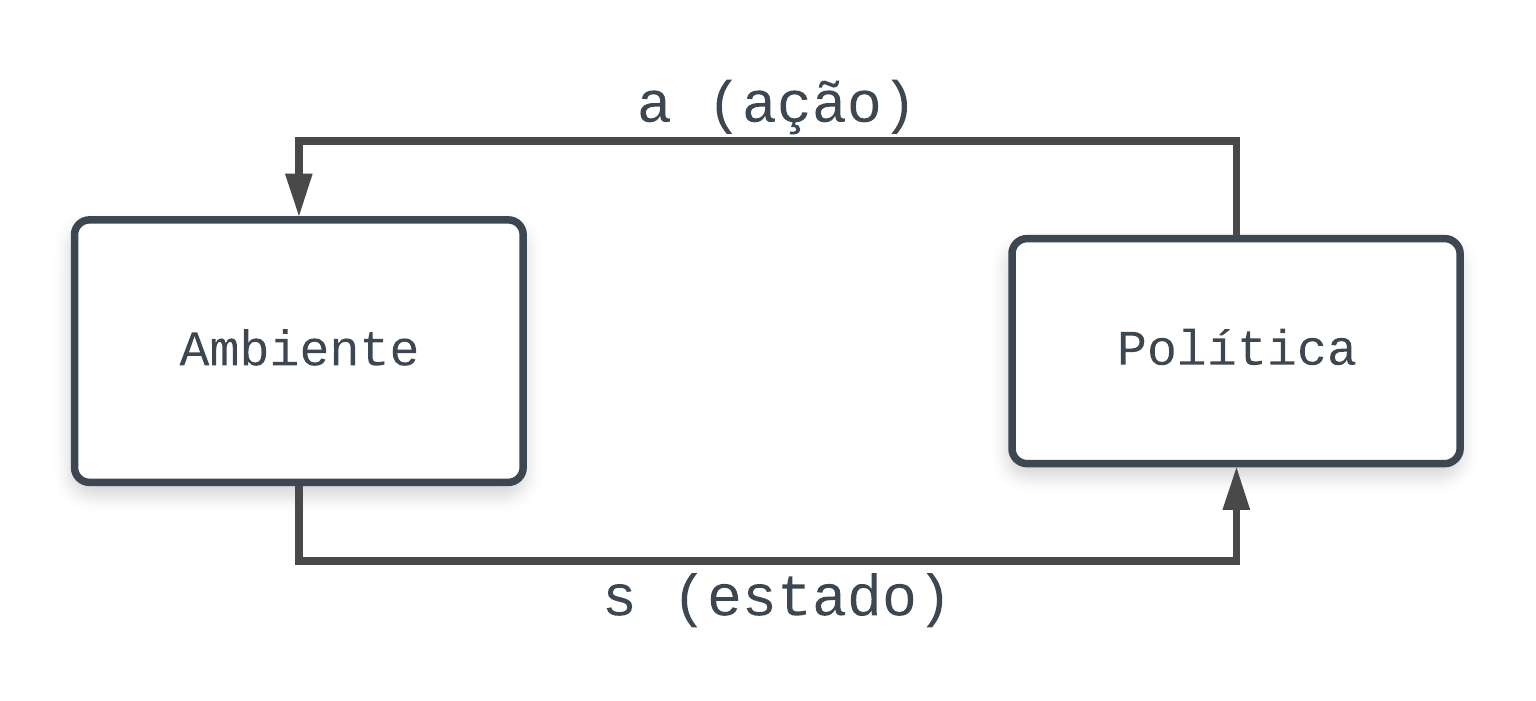
\includegraphics[width=0.65\textwidth]{fluxo_politica_.png}
    \end{center}
    \label{fig:fluxo_politica}
\end{figure}

O objetivo da resolução de um MDP é encontrar uma política $\pi(s) \rightarrow a$
que solucione o problema, ou seja, que diga ao tomador de decisões quais ações
devem ser tomadas em cada estado $s \in S$ de forma que o problema seja
resolvido. Dentre todas as políticas que resolvem um determinado problema, é
considerada uma política \textit{ótima} (denotada $\pi^*$) aquela que segue
algum critério de otimalidade. Normalmente, o critério adotado é o valor
esperado da soma das recompensas retornadas pela série de ações que o agente
toma orientado por aquela política, ou seja, para uma política $\pi^*$ este
valor é máximo. Sua definição pode ser dada por


\begin{equation}
  \pi^* = argmax_\pi\mathbb{E}[\sum_t^TR(s) | \pi]
\end{equation}

 que é a \textit{recompensa esperada total}, ou por

\begin{equation} \label{discounted_expected_reward}
  \pi^* = argmax_\pi\mathbb{E}[\sum_t^T\gamma^tR(s) | \pi]
\end{equation}

que é a \textit{recompensa esperada descontada}, onde $T$ é o horizonte
(conforme descrito na seção \ref{horizonte}) e $R(s)$ é a recompensa pela ação
recomendada ao agente pela política $\pi$ quando este encontra-se no estado
$s$. Há ainda, na fórmula \ref{discounted_expected_reward}, um coeficiente
$\gamma \in ]0,1[$ chamado de \textit{fator de desconto} que serve tanto para
garantir a convergência do valor da recompensa total esperada (em caso de horizonte
infinito, com $T = \infty$), como para regular o impacto que recompensas mais
imediatas exercem na política em relação a recompensas que serão recebidas mais
futuramente.
O fator de desconto $\gamma$ faz parte da \textit{função valor} de uma política,
que dá o valor esperado da recompensa para esta política e que é definida pela
fórmula a seguir:

\begin{equation} \label{value_function}
  V^\pi(s) =  R(s,\pi(s)) + \gamma\sum_{s' \in S}T(s,\pi(s), s')V^\pi(s')
\end{equation}

A fórmula definida em \ref{value_function} é usada na função que define o valor
de uma ação $a$ em um estado $s$ considerando a recompensa imediata de $a$ e
considerando também que as ações subsequentes seguem a política $\pi$. A fórmula
é denotada por $Q$ e é definida por:

\begin{equation}\label{action_value}
  Q^\pi(s,a) = R(s,a) + \gamma\sum_{s' \in S}T(s'|s,a)V^\pi(s')
\end{equation}


Mesmo definindo matematicamente o problema de aprendizado por reforço em
através de um MDP e definindo os conceitos de função valor e  política ótima,
resta saber como buscar uma política que além de resolver o problema, seja uma
política ótima.
Há soluções exatas e aproximadas para o problema, e algumas delas serão
discutidas a seguir.


\section{Métodos de resolução de um MDP}

Resolver um problema definido por um Processo de Decisão de Markov significa
encontrar uma política $\pi$ que, partindo de um estado inicial $s$, faça o
agente eventualmente atingir um estado terminal $s'$. Além disso, normalmente
não se quer apenas encontrar uma política $\pi$ que resolva o problema, mas uma
política ótima $\pi*$ que, além de oferecer ao agente um comportamento que
resulte na resolução do problema, obedeça a algum critério de otimalidade,
normalmente relacionado ao valor total da soma das recompensas recebidas.

Há diversos métodos que encontram tais políticas. Os mais simples, entretanto,
envolvem soluções que utilizam programação dinâmica para encontrar a política de
maior valor através da varredura de todos os estados do conjunto $S$ e de todas
as transições da função $T$, como é o caso no método de \textit{iteração de
valores} \cite{ValueIteration}. Neste caso, o algoritmo é de \textit{model-based}
(baseado em modelos), uma vez que o a modelagem do problema (ou seja, os
próprios componentes da tupla que define o MDP) é utilizada para encontrar a
política que o soluciona.

Há casos, entretanto, que as transições de $T$ e o conjunto $S$ não estão
disponíveis, como é o caso de Processos de Decisão de Markov Parcialmente
Observáveis (POMDP), utilizados para a modelagem de uma série de problemas onde
o estado $s$ é oculto ao agente \cite{Cassandra1998}. Quando o aprendizado se
dá exclusivamente a partir da observação
das recompensas recebidas a partir das ações tomadas em cada estado, se diz que
o método é livre de modelos (\textit{model-free}, em inglês), uma vez que a
busca por um comportamento ótimo se dá mais explicitamente por métodos que
envolvem tentativa e erro. Dos métodos livres de modelo, o mais conhecido se
chama \textit{Q-Learning}, descrito a seguir.

%
% \subsection{Iteração de Valores}
%
% % http://www.iumj.indiana.edu/IUMJ/FULLTEXT/1957/6/56038
% % \cite{Bellman1957}
%
% Este algoritmo baseia-se no conceito de \textit{função valor} de uma política,
% que é uma função $V_\pi: S \mapsto \mathbb{R}$ que dá o valor
% esperado da recompensa total para esta política, partindo de um estado $s \in S$.
% Sua definição formal é:
%
% \begin{equation} \label{value_function}
%   V^\pi(s) = R(s, \pi(s)) + \gamma\sum_{s' \in S}T(s'|s, \pi(s))V^\pi(s')
% \end{equation}
%
% % https://seer.ufrgs.br/rita/article/viewFile/rita_v14_n2_p133-179/3544
% Para cada estado $s \in S$, o algoritmo usa programação dinâmica para determinar
% o valor $V^*(s)$, que é a função valor para uma política ótima. O algoritmo é
% mostrado abaixo em pseudocódigo:
%
%
%
% \begin{algorithm}
% \label{value_iteration_alg}
% \caption{Algoritmo de Iteração de Valores}
%
% \textbf{Entrada:}  Um MDP $(S, A, T, R)$
%
%
% \textbf{Saída:} Uma função V para o MDP dado como entrada
%
%
% \begin{algorithmic}[1]
% \Function{Value Iteration}{MDP}
%   \ForEach{$s \in S $}
%     \State $V_0(s) \gets \max_{a \in A}R(s, a)$
%   \EndFor
%   \State $i \gets 1$
%
%   \Repeat
%     \State $\Delta \gets 0$
%     \ForEach{$s \in S $}
%       \State $v \gets V_i(s)$
%       \State $V_i(s) \gets \max_{a \in A}[R(s, a) + \gamma\sum_{s' \in S}
%        T(s' | s, a)V_{i-1}(s')]$
%        \State $\Delta \gets \max(\Delta, |v - V_i(s)|)$
%     \EndFor
%     \State $i \gets i + 1$
%   \Until {$ \Delta < \epsilon $}
%   \State \Return V
% \EndFunction
% \end{algorithmic}
% \end{algorithm}
%
% O algoritmo baseia-se em um mapeamento $h: S \times A \times V \mapsto
% \mathbb{R}$, tal que $h(s, a, V)$ fornece o valor de executar a ação $a$ no
% estado $s$ seguindo uma política derivada de uma função valor $V$ após esta
% ação:
%
% \begin{equation}
% \label{mapping_h}
% h(s, a, V) = R(s, a) + \gamma\sum_{s' \in S}T(s' | s, a)V(s')
% \end{equation}
%
% O mapeamento descrito em \ref{mapping_h} pode ser usado para definir um operador
%  $H: V \mapsto V$ de melhoria de política, que determina a melhor ação em um
%  estado baseado nos valores V dos estados em uma época de decisão anterior:
%
% \begin{equation}\label{melhoria_politica}
%   HV_k(s) = \max_{a \in A}h(s, a, V_{k+1})
% \end{equation}
%
% O mapeamento definido em \ref{melhoria_politica} pode ser usado para determinar
% a função valor de uma época de decisão a partir da função valor da época de
% decisão anterior:
%
% \begin{equation} \label{value_iteration_equation}
%   \begin{split}
%   V_k(s) & = HV_{k+1}(s) \\
%   & = \max_{a \in A}h(s, a, V_{k+1}) \\
%   & = \max_{a \in A}[R(s, a) + \gamma\sum_{s' \in S}T(s' |s,a)V_{k+1}(s')]
%   \end{split}
% \end{equation}
%
% A equação \ref{value_iteration_equation}, por sua vez, é a base do algoritmo de
% iteração de valores.
%
% \subsection{Iteração de Políticas}
%
% % Howard, Ronald A. (1960). Dynamic Programming and Markov Processes (PDF).
% % The M.I.T. Press.
% % http://web.mit.edu/dimitrib/www/dpchapter.pdf
% Diferentemente do algoritmo de iteração de valores, que busca uma política
% ótima através da exploração do espaço de funções V até que seja encontrada uma
% função valor da qual pode ser obtida uma política ótima, o algoritmo de iteração
% de políticas busca uma política ótima diretamente no espaço de políticas. Além
% da função $V^\pi(s)$, este algoritmo também usa a função $Q^\pi(s,a)$, que
% fornece o valor esperado da recompensa total partindo de uma ação imediata $a$
% em um estado $s$ e seguindo, em estados subsequentes, uma política $\pi$. Sua
% definição é dada por:
%
% \begin{equation}
%   Q_\pi(s,a) = R(s,a) + \gamma\sum_{s \in S}T(s'|s, a)V(s')
% \end{equation}
%
% O algoritmo começa definindo uma política aleatória $\pi'$, determinando o
% valor $V^{\pi'}(s)$. Após, de maneira gulosa, o algoritmo tenta melhorar a
% política encontrada através da busca pela melhor ação para cada um dos estados
% do processo.
%
%
% \begin{algorithm}
% \label{policy_iteration_alg}
% \caption{Algoritmo de Iteração de Políticas}
%
% \textbf{Entrada:}  Um MDP $(S, A, T, R)$
%
%
% \textbf{Saída:} Uma política $\pi'$, otimal para o MDP dado como entrada
%
%
% \begin{algorithmic}[1]
% \Function{Policy Iteration}{MDP}
%   \State Inicialize $\pi$ aleatoriamente
%
%   \Repeat
%     \State $\pi' \gets \pi$
%     \State Avalie a política atual resolvendo o sistema linear:
%     \State $\forall s \in S, V(s) = R(s, \pi'(s)) + \gamma\sum_{s' \in S}
%     T(s'|s, \pi(s))V(s')$
%     \ForEach{$s \in S$}
%       \State $\forall a \in A, Q^{\pi'}(s, a) \gets R(s, a) + \gamma
%       \sum_{s' \in S}T(s' |s, a)V(s')$
%     \EndFor
%     \ForEach{$s \in S$}
%       \State Melhore a política:
%       \State {$\pi(s) \gets argmax_{a \in A}Q^{\pi'}(s, a)$}
%     \EndFor
%   \Until {$ \pi = \pi' $}
%   \State \Return $\pi'$
% \EndFunction
% \end{algorithmic}
% \end{algorithm}
%
% O algoritmo baseia-se no teorema da otimalidade da política, que postula que,
% em uma política $\pi$ com um valor associado $V^\pi$ para um MDP $M$, se a
% política não pode ser melhorada, ou seja, se
%
% $$
% \forall a \in A, V^\pi(s) = \max_{a \in A}Q^\pi(s, a)
% $$
%
% então $\pi$ é otimal para $M$.
%
% Para cada estado $s$, portanto, o algoritmo de iteração de políticas determina
% qual a melhor ação a ser tomada, definindo assim uma nova política $\pi$, dado
% que as ações seguintes serão tomadas de acordo com $\pi'$, a política definida
% no passo anterior, desta forma:
%
% \begin{equation}
%   \forall s \in S, \pi(s) = \arg \max_{a \in A}Q^{\pi'}(s, a)
% \end{equation}


\subsection{Q-Learning}
Há situações onde é praticamente impossível (ou ao menos excessivamente custoso)
buscar uma política otimal para um MDP através de um algoritmo baseado em modelos,
em parte porque o espaço de ações e estados é
muito grande, contribuindo para o custo computacional da busca por uma solução,
e em parte porque algoritmos do tipo
assumem que o agente possui conhecimento sobre o domínio no qual está atuando,
ou seja, é presumido que o agente sabe de antemão as transições entre estados.

% https://arxiv.org/pdf/1301.6718.pdf
% http://idm-lab.org/bib/abstracts/papers/aaai93.pdf
Para resolver este problema, há um algoritmo alternativo chamado Q-Learning
\cite{Wattkins1989} que,
% https://link.springer.com/content/pdf/10.1007%2FBF00992698.pdf
ao invés de buscar uma política ótima calculando diretamente valores para a
função $Q(s, a)$ para todos os estados e ações de um MDP, busca aproximar, de
maneira iterativa, os valores para a função $Q(s, a)$ para os estados e ações do
sistema através de uma busca baseada em tentativa e erro, uma vez que o algoritmo
não supõe que o agente possui quaisquer informações acerca das transições entre
estados e das recompensas associadas a elas.


A ideia fundamental do algoritmo Q-Learning é, portanto, a aproximação dos
valores para a função $Q$ através dos valores $Q(s, a)$ que são observados na
medida em que o agente interage com o ambiente. Tais valores (chamados de
\textit{Q-values}) são salvos em uma matriz de tamanho $|S| \times |A|$ (
normalmente discretiza-se representações contínuas, como quando um estado é
representado por um número real) chamada de \textit{Q-table} e são
sucessivamente atualizados para valores cada vez mais próximos dos valores
verdadeiros da função $Q(s, a)$. Os valores da \textit{Q-table} são atualizados
com base na seguinte fórmula:

\begin{equation}
  \label{q_learning_update}
  Q_{t+1}(s, a) = (1 - \alpha)Q_t(s, a) + \alpha(R(s, a) + \gamma\max_{a \in A}Q'(s', a))
\end{equation}

Onde $\alpha$ é chamado de \textit{coeficiente de aprendizado}, que diz qual o
peso do novo valor observado ante o \textit{Q-value} guardado na tabela, oriundo
de observações anteriores.

O algoritmo de Q-learning é definido pelo pseudocódigo presente no algoritmo
\ref{q_learning_alg}.


\begin{algorithm}
  \label{q_learning_alg}
\caption{Algoritmo de Q-learning}

\textbf{Entrada:}  Um MDP $(S, A, T, R)$ e um coeficiente de aprendizado $\alpha$


\textbf{Saída:} Uma função $Q$, aproximação de $Q*$


\begin{algorithmic}[1]
\Function{Qlearning}{MDP}
  \State Inicialize $Q: S \times A\mapsto \mathbb{R} $ aleatoriamente

  \Repeat
    \State Inicialize o agente em um estado inicial $s \in S$
    \While {\textit{$s$ não é um estado terminal}}
      \State Calcular $a$ de acordo com a política atual de exploração (e.g. $\arg \max_a Q(s,a)$)
      \State $s' \gets T(s, a)$
      \State $Q(s', a) \gets (1 - \alpha)\cdot Q(s,a) + \alpha \cdot (r + \gamma\max_{a' \in A}Q(s', a'))$
      \State $s \gets s'$
    \EndWhile
  \Until {\textit{critério de convergência de Q seja atingido}}
\EndFunction
\end{algorithmic}
\end{algorithm}

\subsubsection{Política de exploração em Q-Learning}
Na linha 6 do algoritmo \ref{q_learning_alg}, uma ação, dentre todas as
possíveis ações para o estado no qual o agente se encontra, deve ser escolhida.
Mas, em um estado inicial, apenas com valores gerados aleatoriamente para a
\textit{Q-table}, como o agente deve decidir qual a melhor ação a ser tomada? E
mais: após algumas iterações, quando já se sabe que algumas sequências de ações
geram as melhores recompensas (por trazerem na \textit{Q-table} os melhores
valores para as aproximações da função $Q$), como saber se outras sequências,
ainda não exploradas, não resultam em recompensas totais maiores? A cada
momento, portanto, o agente deve decidir se busca melhorar as sequências de
ações já encontradas até o momento através do seu refinamento (o que é chamado de
\textit{exploitation}) ou se busca sequências de ações completamente novas, na
esperança de que elas resultem em recompensas totais maiores (o que é chamado de
\textit{exploration}). O problema que trata dessa decisão a ser feita pelo
agente é chamado de \textit{exploration/exploitation trade-off} ou de \textit{
exploration/exploitation problem}. A solução para esse problema proposta em
[citation] é simples: há um fator $\epsilon \in (0,1)$ que determina a
probabilidade de, a cada época de decisão, o agente não seguir os valores da
\textit{Q-table} e, ao invés disto, executar uma ação aleatória dentre todas as
outras possíveis para aquele estado. No começo da interação do agente com o
ambiente, quando a maioria das células da \textit{Q-table} ainda guardam os
valores gerados aleatoriamente no primeiro passo do algoritmo, $\epsilon$ guarda
um valor próximo de 1, fazendo com que o agente tome uma decisão aleatória (e,
consequentemente, exploratória) na grande maioria das vezes. À medida que o
agente atualiza os valores da \textit{Q-table}, entretanto --- reunindo, desta
maneira, mais conhecimento sobre o sistema ---, o valor de $\epsilon$ decai,
fazendo com que o agente passe, gradativamente, a tomar mais decisões baseadas
nos valores da \textit{Q-table}.

% "Learning from Delayed Rewards" - a tese do watkins


\subsection{Aprendizado por Reforço com Redes Neurais Profundas}
\label{dqn}
% [1] https://arxiv.org/pdf/1312.5602.pdf - atari2013
% [2] NIPS2012_4824
%
% [3] Silver2016
% [4] 705737

% https://www.cs.toronto.edu/~vmnih/docs/dqn.pdf
% https://storage.googleapis.com/deepmind-media/dqn/DQNNaturePaper.pdf
% https://arxiv.org/pdf/1612.00380.pdf
O algoritmo chamado de \textit{Deep Q-Learning} tem este nome porque combina
\textit{Q-Learning} com redes neurais profundas (\textit{deep neural networks}).
Seu funcionamento é parecido com \textit{Q-Learning}, com a diferença de que, ao
invés serem guardados em uma tabela, os valores aproximados para a função
$Q^*(s, a)$ são fornecidos a uma rede neural profunda, que usa os valores
dados a ela para aproximar a função $Q^*$. Possui a vantagem da escalabilidade,
uma vez que sistemas onde os estados possuem muitas dimensões (ou há muitas
ações possíveis para cada estado) requerem tabelas que, na prática, acabam se
tornando inviáveis, no que tange ao consumo de recursos computacionais (e.g.
memória). Em \cite{atari2013}, uma rede neural profunda foi treinada para jogar jogos da
plataforma Atari: neste trabalho, o estado é representado pelos componentes
visuais do jogo, ou seja, pela imagem formada na tela. Quatro quadros
consecutivos do jogo são transmitidos a uma rede neural convolucional \cite{NIPS2012_4824},
como registrado na figura \ref{fig:doom_neural_network}, que
tenta aproximar, para cada ação possível, seu valor $Q$, sendo tomada a ação de
maior valor. O algoritmo aproveita-se do fato de que, em um jogo, há um número
muito limitado de ações possíveis para cada estado: mover-se ou disparar uma
arma por exemplo. Os treinamentos resultaram em performances próximas da humana
em todos os jogos para os quais redes foram treinadas.

\begin{figure}[h]
    \caption{Esquema de uma rede neural para o jogo \textit{Doom}.}
    \begin{center}
      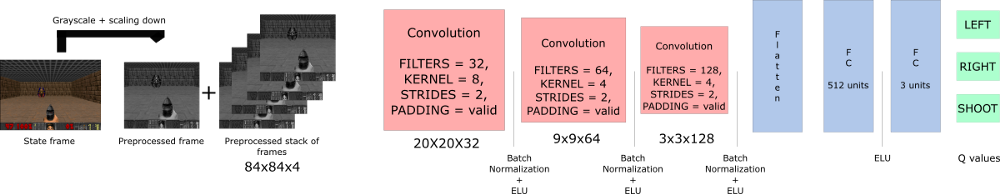
\includegraphics[width=0.9\textwidth]{cnn_doom.png}
    \end{center}
    \label{fig:doom_neural_network}
\end{figure}

Talvez o exemplo mais famoso de aplicação que combinou algoritmos clássicos de
aprendizado por reforço com redes neurais profundas tenha sido o AlphaGo \cite{Silver2016}.
Desenvolvido pela empresa DeepMind, o AlphaGo é um \textit{software} que joga o
jogo de tabuleiro Go, original da China e talvez um dos jogos de tabuleiro mais
antigos do mundo. Ensinar programas de computador a jogar Go nunca foi uma
tarefa tão simples como jogar xadrez, por exemplo, uma vez que o número de
jogadas possíveis em uma rodada é muito maior, tornando buscas que usam árvores
para representar jogadas futuras praticamente inviáveis \cite{705737}. Este problema,
entretanto, foi contornado pelos pesquisadores da DeepMind através de um
algoritmo que combina buscas guiadas por políticas com redes neurais profundas,
e o resultado foi uma série de vitórias contra campeões continentais e mundiais
da modalidade. Tais feitos não seriam possíveis, entretanto, se não houvesse
alguma maneira de representar o jogo em um ambiente virtual, seja o jogo feito
para a plataforma Atari ou o jogo de tabuleiro, e trabalhos como os citados aqui
só são possíveis com o uso de simuladores.



\section{Simuladores de AR}
\label{simuladores_ar}
% [1] ng2003
% [2] tese do andrew ng, link em algum lugar no texto
% [3] artigo do mujoco
% [4] DMControl
\begin{figure}[h]
    \caption{Um robô real e sua versão modelada em um simulador.}
    \begin{center}
      \frame{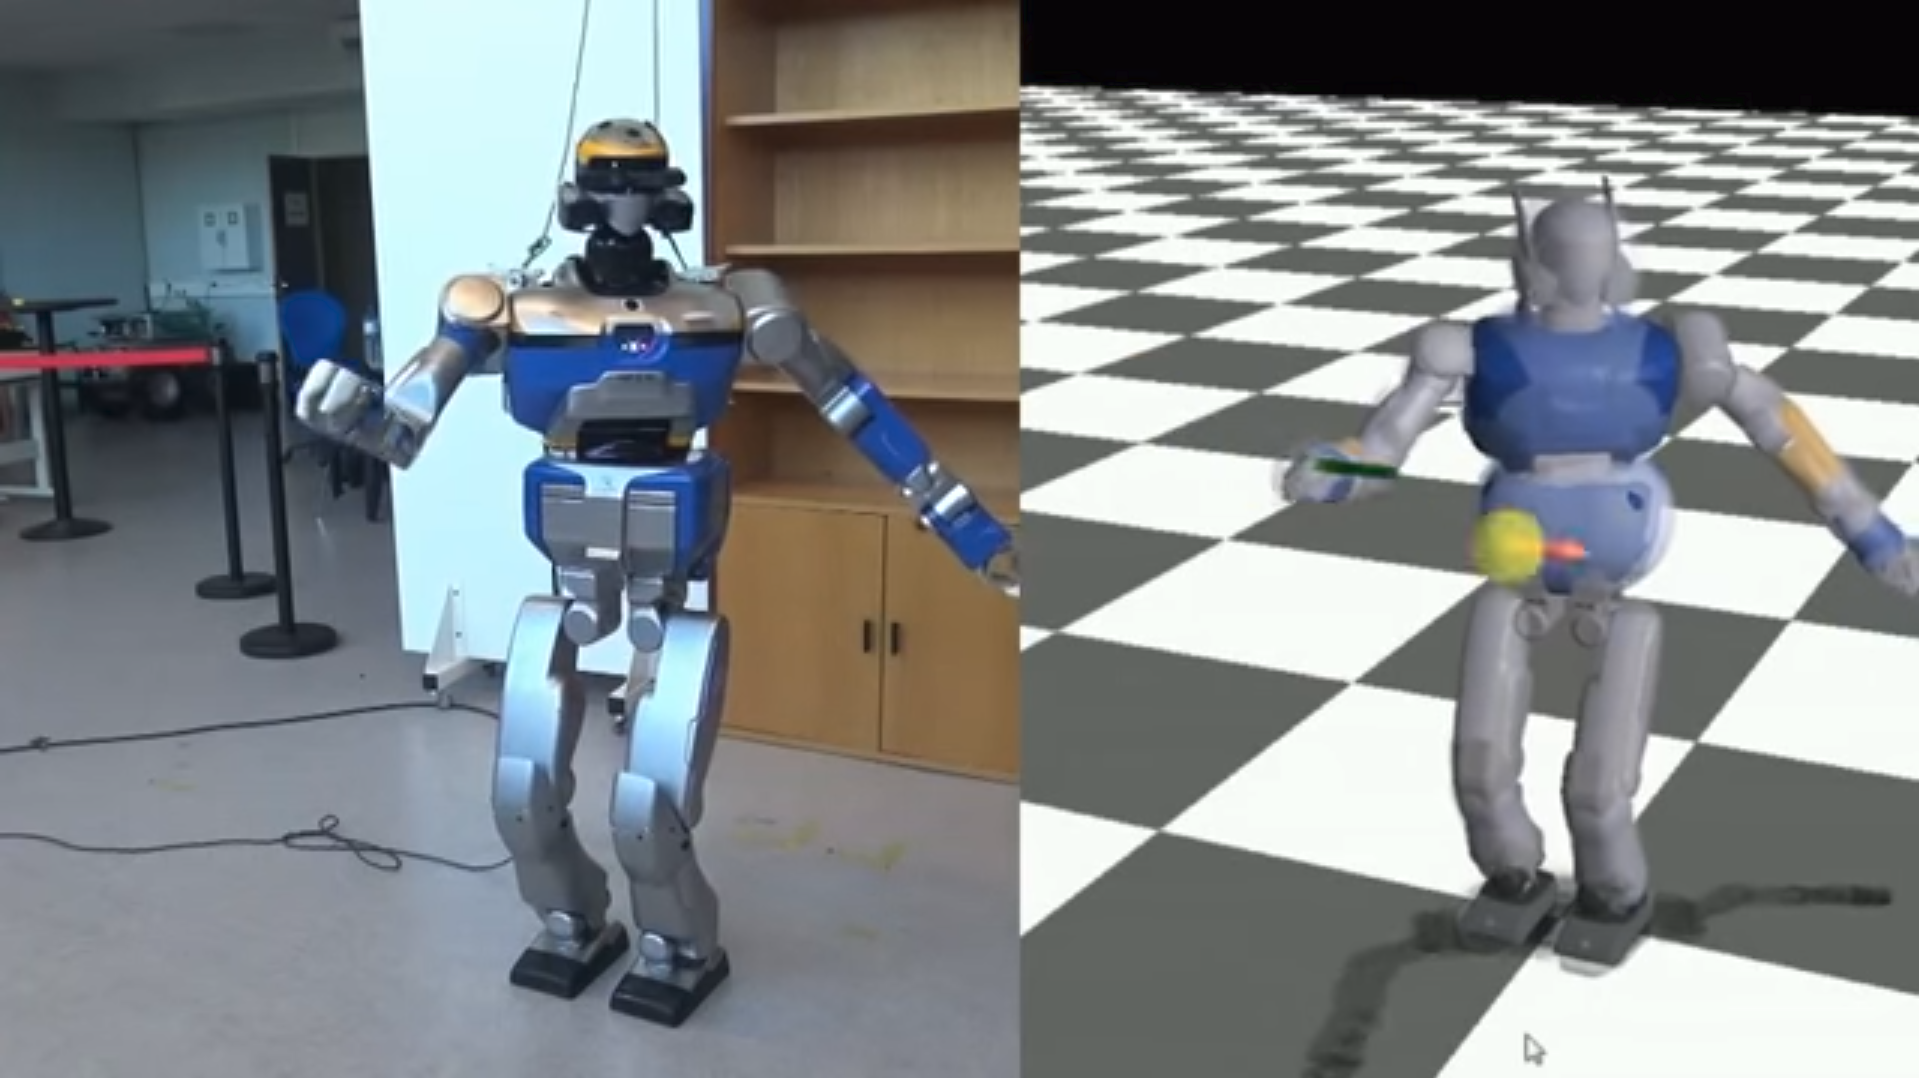
\includegraphics[width=0.9\textwidth]{mujocosimulator.png}}
    \end{center}
    \label{fig:mujocosimulator}
\end{figure}

Conforme mencionado anteriormente, algoritmos de aprendizado por reforço
possuem diversas aplicações; seja em jogos de tabuleiro ou de
\textit{video games} \cite{AlphaGoEvolution2016,ALE,VizDoom} ou sistema de
controle de veículos autônomos \cite{Ng2003},
algoritmos de aprendizado por reforço são recomendados em quaisquer situações
onde ações devem ser tomadas em sequência, dentro de um ambiente. Um problema
surge, entretanto, quando torna-se necessário modelar um ambiente sob a forma de
um Modelo de Markov ou sob qualquer outra forma que possa ser compreendida por
um programa de computador. No caso do AlphaGo, o tabuleiro e as peças precisavam
ser representados em um \textit{software} para que o agente em treinamento
pudesse lê-los e compreendê-los; no caso trabalhado por Andrew Ng \cite{Ng2003},
uma representação do veículo automotor precisa ser modelada, para que o
comportamento que mantém o veículo estabilizado possa ser aprendido com a ajuda
dos métodos propostos pelo trabalho.


No caso da robótica, o uso de simuladores possui ainda outra vantagem prática:
modelar robôs em um ambiente simulado que segue as leis da física do mundo real
permite, por exemplo, que um modelo de um robô passe por um treinamento virtual
antes de ser construído no mundo real (como na figura \ref{fig:mujocosimulator}),
acelerando, desta maneira, o processo de treinamento. Há diversas ferramentas
que são utilizadas especialmente para construir simulações que apresentem
características físicas semelhantes às do mundo real: motores de física como o
MuJoCo \cite{MuJoCo}, por exemplo, fornecem uma das bases para o
\textit{software} da DeepMind \cite{DMControl}, que pode ser utilizado para a
modelagem de problemas de robótica.


\subsection{Definição de um simulador}
Em sua definição de dicionário, um simulador é "uma máquina com um conjunto de
controles designada para proporcionar uma imitação realística da operação de um
veículo, aeronave ou outro sistema complexo, usado para fins de treinamento". Um
simulador, portanto, é um sistema capaz de criar um ambiente virtual cujas
características aproximem-se, com certo grau de fidelidade, das condições
apresentadas por um ambiente real. Tomemos as autoescolas do Brasil como
exemplo: nelas, entre o fim das aulas teóricas e o começo das aulas práticas,
dadas em um veículo real, simuladores (figura \ref{fig:simuladorautoescola}) são
utilizados por alunos para que os princípios básicos de direção sejam aprendidos
sem o risco de acidentes.


Obviamente, os simuladores de direção não são uma representação completamente
fiel de um automóvel de verdade, mas são uma aproximação fiel o suficiente para
que aquele que almeja adquirir sua carteira de habilitação possa embarcar em um
automóvel sabendo ao menos o básico de como guiá-lo. Aqui, há uma espécie de
troca entre fidelidade e segurança: obviamente os simuladores de direção não
apresentam ao seu usuário todas as nuances de um automóvel e todas as
particularidades do trânsito, afinal o simulador possui caráter introdutório e
apenas uma parte das inúmeras situações que um motorista enfrenta é apresentada.
Há a vantagem da segurança, entretanto: no momento em que o motorista em
formação embarca em um veículo verdadeiro, os conhecimentos básicos necessários
para dirigir já foram adquiridos, o que reduz o risco de acidentes causados por
falta de preparo por parte do aluno. Além das questões relacionadas a segurança
no trânsito, em um simulador de direção, situações corriqueiras do trânsito
podem ser ensaiadas, sem que o aluno tenha que vivenciá-las na prática. Isto
fornece aos preparadores um grau maior de controle sobre os diferentes desafios
que são apresentados àqueles que pretendem obter sua licença para dirigir:
cenários que ocorrem com pouca frequência, por exemplo, podem ser apresentados
em um simulador repetidas vezes para o aluno, até que este adquira o domínio
necessário para enfrentar a mesma situação na prática.

\begin{figure}[h]
    \caption{Simulador usado em autoescolas brasileiras.}
    \begin{center}
      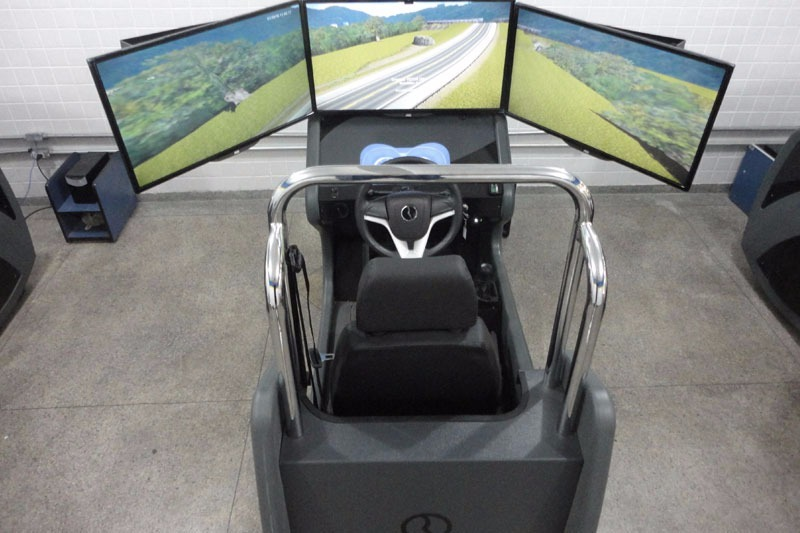
\includegraphics[width=0.9\textwidth]{simuladorautoescola.jpg}
    \end{center}
    \label{fig:simuladorautoescola}
\end{figure}


Da mesma maneira, no trabalho apresentado em \cite{Ng2003}, uma modelagem
virtual das diferentes propriedades do helicóptero lidas pelo \textit{software}
de controle é construída. Neste ambiente simulado, alimentado com dados
resultantes de um experimento onde o helicóptero é controlado por um piloto
humano, o algoritmo proposto pelo trabalho tenta aproximar-se do comportamento
do piloto, aprendendo a guiar o veículo sem grandes perturbações. Neste caso, fica muito
mais evidente o grau de controle que o simulador fornece aos envolvidos no
projeto de desenvolvimento do veículo: nele, os dados gerados a partir de um
piloto humano podem ser manipulados para forçar o agente a aprender a
comportar-se em diversos tipos de situação. Isto acarreta em uma enorme economia
de tempo e também de recursos, uma vez que, quando um acidente destrutivo ocorre
dentro de um ambiente simulado, não é necessário construir uma nave novamente.



Com base nos exemplos dados acima, é fácil inferir que há vantagens associadas
ao uso de simuladores. O que não fica tão evidente, entretanto, é o custo que a
adoção de tais ferramentas traz consigo: além, obviamente, dos recursos que
devem ser empregados para que se tenha um simulador pronto para uso --- aqui,
podem ser considerados recursos o tempo necessário para desenvolver um simulador
quanto o dinheiro para pagar pela licença de um \textit{software} já pronto ---,
há também o custo relativo ao tempo que é necessário para que sejam dominadas
todas as ferramentas que um simulador oferece. Tais custos, entretanto, trazem
consigo as vantagens observáveis nos dois exemplos apresentados: no caso da
autoescola, o risco de acidentes é reduzido, uma vez que os condutores em
formação já possuem os conhecimentos básicos de direção ao conduzir um veículo
pela primeira vez; no caso do \textit{drone}, por sua vez, o tempo de
treinamento do veículo é reduzido drasticamente, acarretanto em uma economia de
tempo.


O uso de simuladores, assim sendo, traz consigo um custo normalmente associado
a recursos financeiros ou tempo, que precisam ser empregados para que o
\textit{software} seja adquirido ou para que as ferramentas fornecidas por ele
sejam compreendidas e tenham seu uso dominado. Tais custos, entretanto, podem
ser compensados --- ou até mesmo amplamente superados --- pelas diferentes
vantagens trazidas pelo uso de tais ferramentas. Cabe, neste caso, uma análise
minuciosa das vantagens e desvantagens da adoção de simuladores, bem como uma
escolha sensata das diferentes ferramentas disponíveis.


\section{Simuladores de Aprendizado por Reforço}

% [1] Mario2009
% [2] Narasimhan2015


Algoritmos de aprendizado por reforço são recomendados em quaisquer
situações onde ações devem ser tomadas de maneira sequencial por um agente
inserido dentro de um ambiente, com o qual ele interage através da sua sucessão
de decisões tomadas. Problemas diferentes, portanto, requerem diferentes meios
de simulação: um agente que joga xadrez \cite{Chess2017} pode ser treinado
usando-se de um simulador que representa o tabuleiro através de uma matriz, onde
cada célula guarda a informação da peça ali presente, caso haja alguma. Um outro
simulador \cite{Mario2009}, que treina um agente para jogar o jogo
\textit{Super Mario World}, baseia-se em uma adaptação do modo com que os
diferentes níveis do jogo eram representados no \textit{Super Nintendo}, seu
\textit{console} de origem.


Visto que problemas diferentes requerem maneiras distintas de representar-se o
ambiente no qual os agentes estão inseridos e com os quais eles interagem, é
necessário definir a estrutura básica, comum a qualquer simulação, de um
problema de aprendizado por reforço. É natural que, ao pensarmos na palavra
"simulador", nos venha à mente algum tipo de ferramenta essencialmente visual,
como o simulador utilizado em autoescolas da figura
\ref{fig:simuladorautoescola}. Entretanto, quando se trata de aprendizado por
reforço, nem sempre há utilidade em construir visualmente o ambiente e o agente
nele inserido: como no caso do tabuleiro de xadrez, representá-lo através de
figuras visuais é interessante, mas opcional.


Tratanto-se de aprendizado por reforço, portanto, o componente visual nem sempre
faz parte da essência do simulador. Por vezes, é util que este seja ignorado
para que os recursos que seriam consumidos por algoritmos de computação gráfica
sejam transferidos às tarefas ligadas ao treinamento do agente e, em alguns
casos, é até mesmo impossível representar o problema de uma forma essencialmente
visual \cite{Narasimhan2015}. Sendo assim, resta definir qual é o elemento
fundamental de um simulador, quando dentro de um contexto de treinamento de
agentes através de algoritmos de aprendizado por reforço.

\begin{figure}[ht]
    \begin{center}
      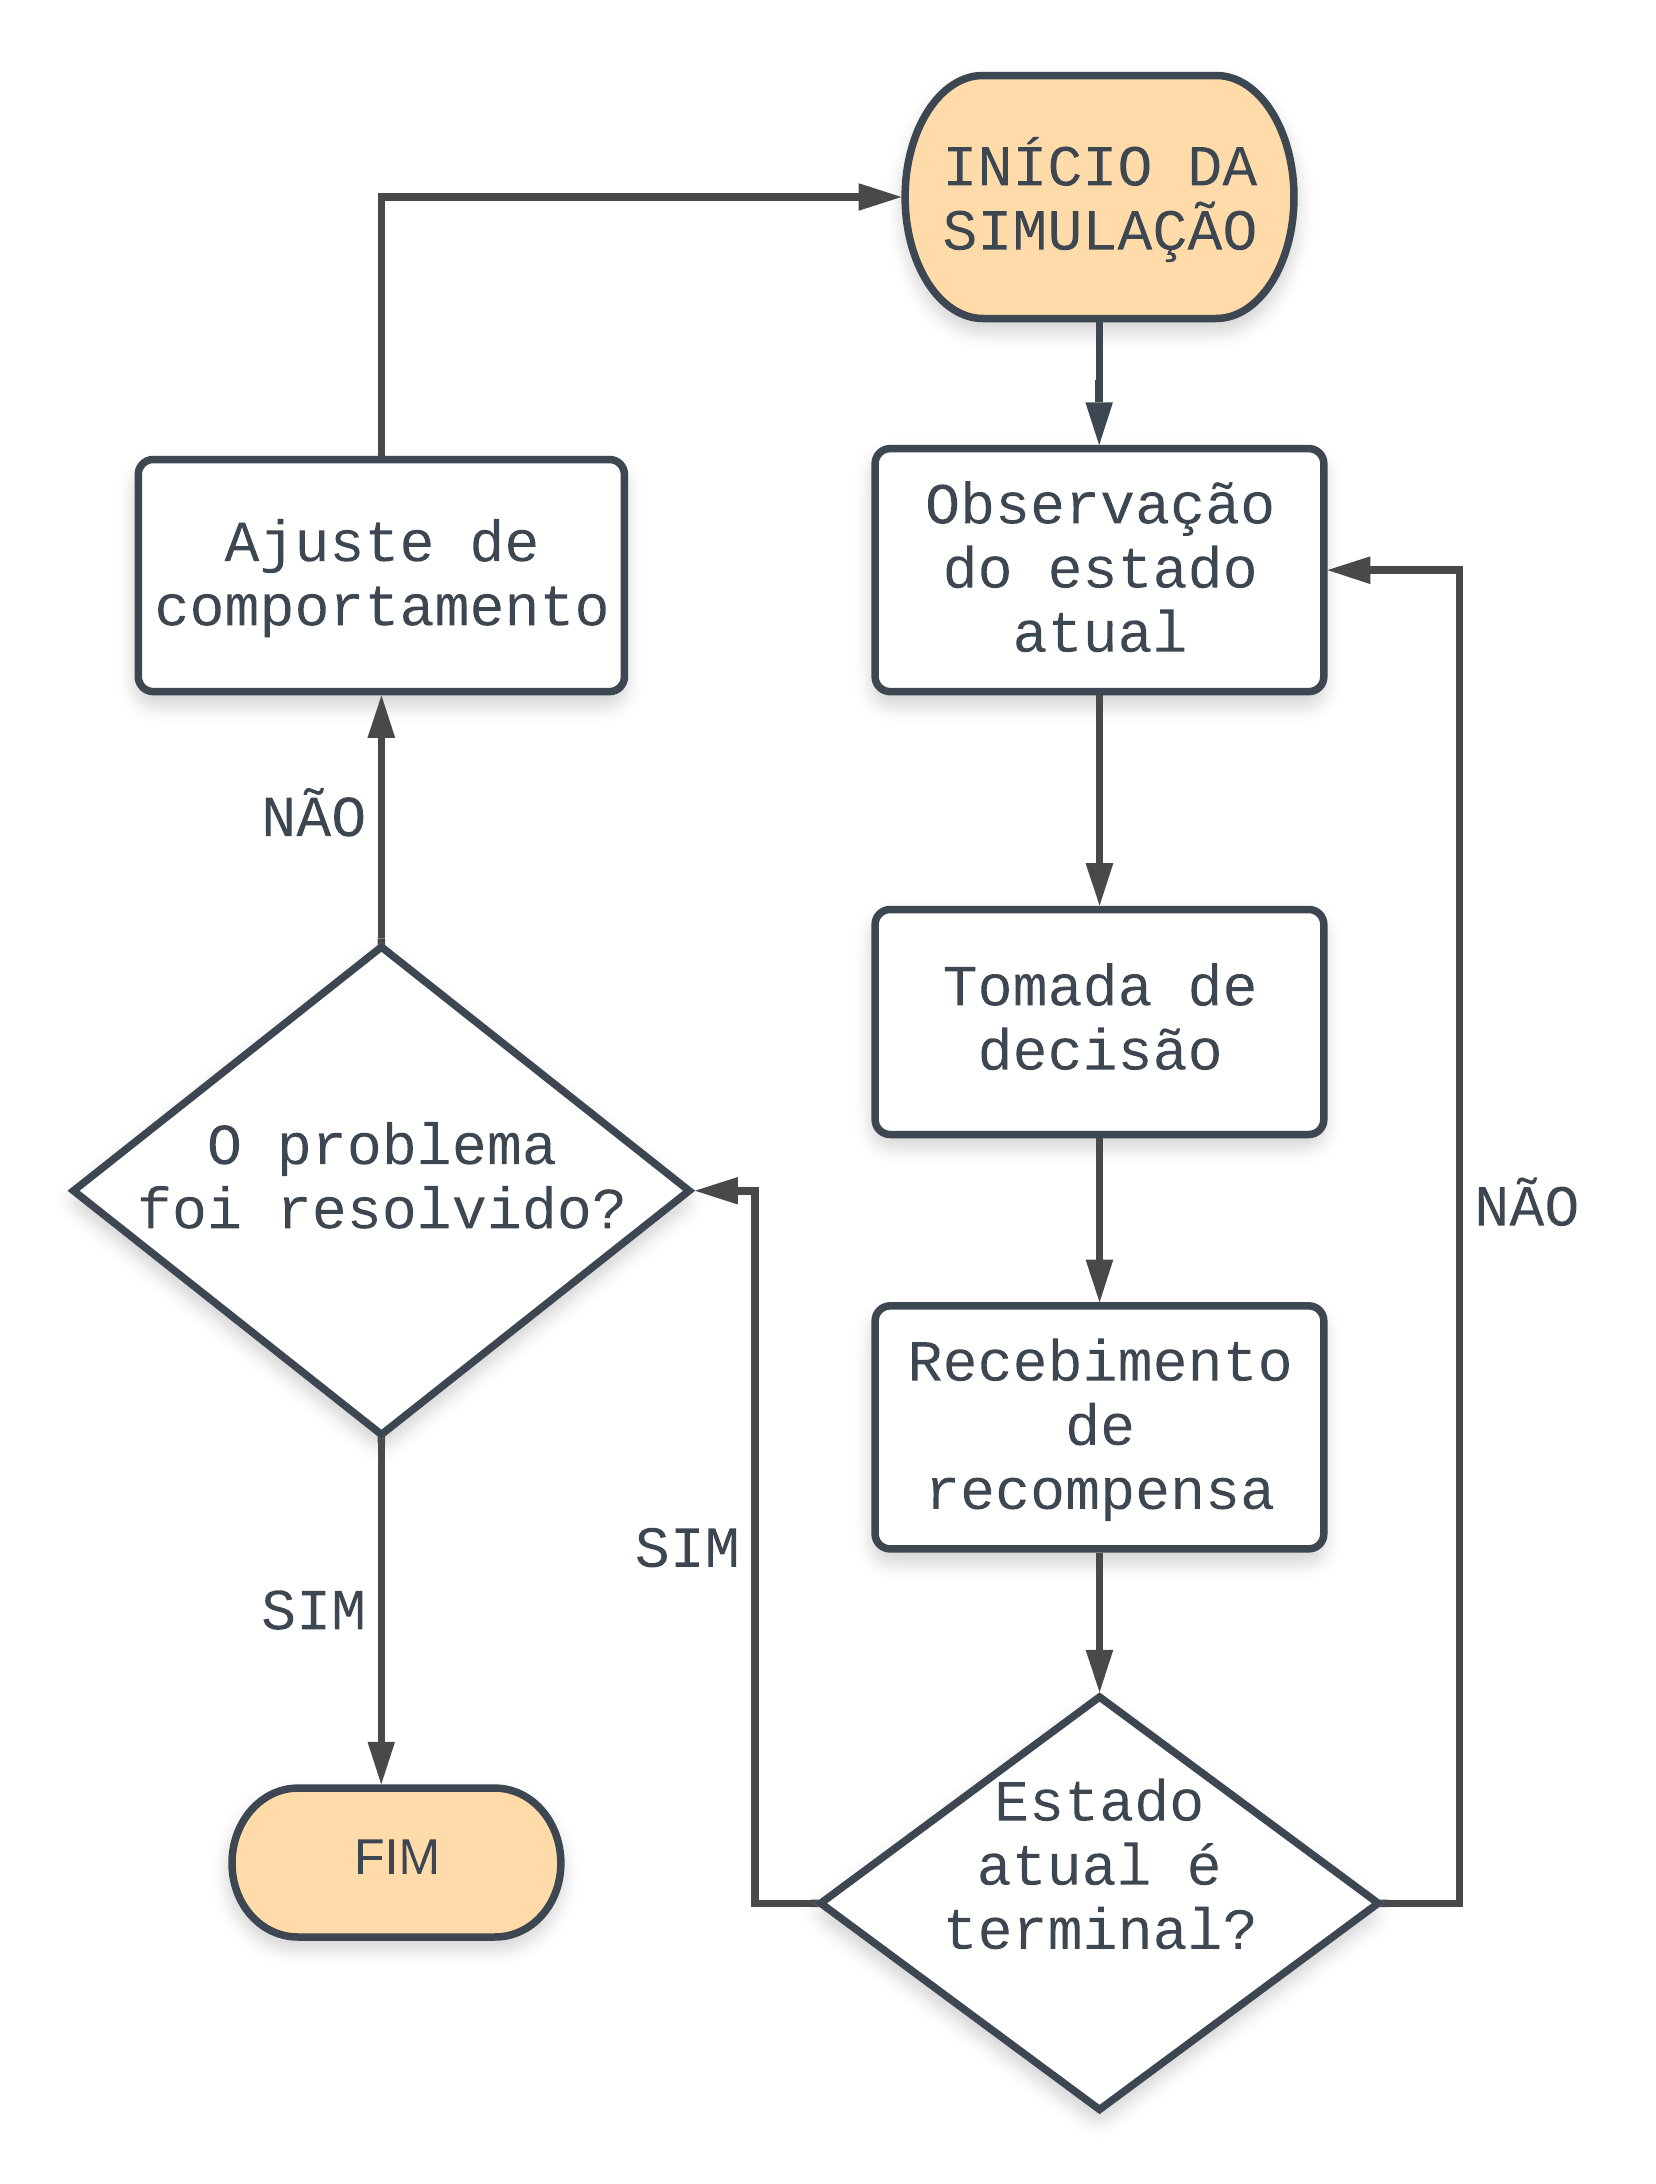
\includegraphics[width=0.5\textwidth]{fluxo_ar.png}
    \end{center}
    \caption{Ciclo de aprendizado do agente via interação com o ambiente}
    \label{fig:fluxo_ar}
\end{figure}


E qual é a peça principal de um sistema modelado por um Processo de Decisão de
Markov? Bom, é natural que seja, exatamente, o MDP e seus componentes: as
informações a respeito do ambiente, as ações possíveis que podem ser tomadas em
um estado, a noção de recompensa e as transições entre estados. O componente
fundamental de uma simulação de aprendizado por reforço é, portanto, a
representação dos elementos que compõem um Processo de Decisão de Markov e das
relações que estes elementos possuem entre si, como as transições entre estados
decorrentes das ações tomadas pelo agente e as recompensas recebidas por elas.
A figura \ref{fig:fluxo_ar} mostra o fluxo percorrido durante o treinamento de
um agente de aprendizado por reforço, e é justamente a implementação dos
estágios deste fluxo que compõem o sistema fundamental de treinamento de um
agente de AR.


Um simulador de aprendizado, portanto, combina o ciclo descrito na figura
\ref{fig:fluxo_ar} com ferramentas que permitem que sejam representados os
componentes de um MDP: o ambiente, o agente nele inserido, as ações possíveis
em cada estado e a noção de recompensa, sem que, necessariamente, haja uma
representação visual destes. A ferramenta \textit{VizDoom} \cite{VizDoom}, por exemplo,
permite que algoritmos de aprendizado por reforço sejam aplicados ao jogo de
tiro em terceira pessoa \textit{Doom}, tendo se tornado uma ferramenta
importante de avaliação de algoritmos de AR. Há evidentemente, uma construção
visual dos objetos (i.e. o jogador, o mapa e os inimigos), mas também há, no
cerne do \textit{software}, estruturas de dados internas que representam o
estado atual do jogo e das quais o agente extrai as informações necessárias para
suas tomadas de decisão. Acima destas estruturas, o treinamento do agente é
realizado seguindo-se o fluxo da figura \ref{fig:fluxo_ar}.



\subsection{Estrutura simulador de aprendizado por reforço}


\begin{figure}[h]
    \caption{O problema conhecido como \textit{Frozen Lake}}
    \begin{center}
      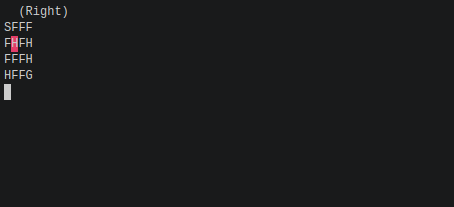
\includegraphics[width=0.5\textwidth]{frozen_lake.png}
    \end{center}
    \label{fig:frozen_lake}
\end{figure}


Para construir um simulador de AR, conforme desenvolvido anteriormente, não é
estritamente necessária a presença de um componente visual. É preciso,
entretanto, que a arquitetura do simulador contenha os componentes de um MDP e
que as relações entre eles se deem corretamente, em um ciclo próximo do que é
descrito na imagem \ref{fig:fluxo_ar}. Estas são as premissas básicas para a
construção de um simulador de aprendizado por reforço e qualquer construção que
vá além desta definição irá depender da natureza do problema a ser resolvido, o
que pode exigir o uso de ferramentas mais complexas, como motores de física, que
buscam aproximar o comportamento de corpos no espaço tridimensional da maneira
como ocorre no mundo real, ou o emprego de ferramentas mais simples. Um exemplo
de problema bastante trivial, que pode ser construído em um simulador sem que
seja necessário nada além de estruturas básicas de dados e representação visual
em modo texto é um problema chamado \textit{Frozen Lake} \cite{FrozenLake}: o problema descreve
um homem que precisa andar por sobre um lago congelado, saindo de um ponto de
partida e com destino a um ponto de chegada, previamente conhecido. O lago
apresenta lugares,
porém, onde a camada de gelo é fina demais para suportar o peso do homem, que
cairá na água caso tente passar por eles. Cabe ao agente, portanto, aprender a
controlar o homem por sobre o lago, sabendo de onde ele sai, para onde ele deve
se dirigir e quais pontos no lago não podem ser perpassados. Para representar o
lago, apenas uma matriz de caracteres é necessária, com símbolos distintos para
representar o ponto de partida, o ponto de chegada, os pontos onde é seguro
atravessar e os pontos onde o gelo é fino demais. Uma matriz de tamanho
arbitrário, descrita na tela de um \textit{console}, portanto, é capaz de
fornecer uma representação completa do problema, como é o caso na imagem
\ref{fig:frozen_lake}.


Cabe esclarecer, entretanto, que o caso do problema \textit{Frozen Lake} é
bastante especial, uma vez que o problema é comumente utilizado apenas para fins
didáticos, como exemplo de uso de técnicas simples de resolução de Processos de
Markov como as exibidas no capítulo \ref{basic_concepts}. É natural que o uso
de simuladores mais complexos, que tenham a capacidade de representar estados
definidos por um volume maior de informações, sejam empregados quando o problema
em questão envolve mais elementos do que uma simples matriz que representa um
lago congelado.


É este o caso no ramo da robótica, por exemplo. Qualquer tarefa que necessite
ser executada repetidamente e com certo grau de precisão é uma boa candidata
para a automatização através do emprego de robôs: linhas de montagem de
empresas automotivas, por exemplo, já são dominadas por robôs há varios anos.
Outras tarefas, mais complexas do que as executadas pelos robôs da manufatura,
mas ainda assim consideradas maçantes e repetitivas por humanos --- como
dirigir, por exemplo ---, também são fortes candidatas à automação, tendo, nos
últimos tempos, sido alvo de pesquisas de ponta envolvendo inteligência
artificial, com a popularização de técnicas de aprendizado de máquina e visão
computacional. É aí que entra o uso de simuladores: durante as fases iniciais
de desenvolvimento de um robô, uma versão virtual deste pode ser construída,
como na figura \ref{fig:mujoco_robot}, em um ambiente fundamentado em motores
de física que simulam as leis do mundo real. No ambiente controlado de um
simulador, o treinamento do agente pode ser feito de forma acelerada, fazendo
com que as primeiras versões reais do robô já apresentem uma versão incial do
comportamento que quer-se ensinar a ele.


No capítulo a seguir, serão discutidas as diferentes formas de implementar-se
uma simulação de um problema de aprendizado por reforço, bem como as ferramentas
que podem ser utilizadas para este fim. Também é apresentada uma hierarquia,
mostrando o grau de complexidade de cada uma das ferramentas.



%
% Além da economia de tempo e da liberdade para modelar de forma controlada
% diferentes tipos de ambiente com comportamento estocástico, simuladores também
% oferecem uma maneira de analisar o desempenho de diferentes algoritmos de
% aprendizado quando aplicados ao mesmo problema, ou o contrário, que ocorre
% quando um mesmo algoritmo de aprendizado é aplicado a problemas diferentes a fim
% de que possa ser avaliada a sua generalidade.



% Aprendizado por reforço lida com problemas onde um agente, inserido em um
% ambiente, tenta resolver um determinado problema através de uma série de ações.
% Em alguns problemas, é de interesse do responsável pelo desenvolvimento do
% agente que se possa modelar casos nos quais o agente está inserido em um
% ambiente estocástico (i.e. que apresenta fatores aleatórios que influenciam em
% seu comportamento).
%que desempenhe o papel de um sistema
% No problema trabalhado por Andrew Ng \bruno{add citation}, por exemplo,
% um agente é treinado para ser capaz de controlar um helicóptero, a fim de
% estabilizá-lo levando em consideração fatores imprevisíveis do sistema (e.g.
% vento, chuva e demais fatores que podem interferir na estabilidade do veículo).
% Nota-se que o problema, portanto, tem um objetivo prático: desenvolver um
% controle para um helicóptero que mantenha sua estabilidade, independentemente
% de fatores externos. O problema surge na necessidade de treinar o agente: como
% proceder com o treinamento em ambientes que possuam diferentes níveis de
% imprevisibilidade e cujos fatores como chuva e vento atuem em diferentes
% intensidades? Logicamente, o objetivo final do processo é ter um veículo
% autocontrolado capaz de manter sua estabilidade sob qualquer tipo de interpérie;
% para que isso seja possível, todavia, é necessário que o agente seja treinado
% em diferentes tipos de ambiente, o que pode se tornar inviável dadas restrições
% como o tempo disponível para o projeto e a necessidade dos desenvolvedores de se
% deslocar até locações onde há ambientes ideais para o treinamento. A solução
% que é amplamente usada nesses casos, portanto, é a modelagem de locações em um
% simulador que representa diferentes tipos de terreno e que permite ao
% pesquisador que este configure os diferentes fatores do ambiente de acordo com
%  sua necessidade.

%
%
% Além da economia de tempo e da liberdade para modelar de forma controlada
% diferentes tipos de ambiente com comportamento estocástico, simuladores também
% oferecem uma maneira de analisar o desempenho de diferentes algoritmos de
% aprendizado quando aplicados ao mesmo problema, ou o contrário, que ocorre
% quando um mesmo algoritmo de aprendizado é aplicado a problemas diferentes a fim
% de que possa ser avaliada a sua generalidade. Esse foi um dos objetivos do
% desenvolvimento da plataforma Gym, da OpenAI, uma organização sem fins
% lucrativos que desenvolve projetos com foco em inteligência artificial. Com um
% catálogo de diversos cenários de aprendizado por reforço (chamados de
% \textit{environments}) oriundos da literatura de IA e até mesmo de jogos feitos
% para antigas plataformas de 8 \textit{bits}, esta plataforma oferece uma API
% (Interface Pública de Aplicação, em tradução livre; espécie de ponto de acesso
% ao qual programas podem se conectar, se seguirem um determinado formato) que
% permite que qualquer pessoa desenvolva seu algoritmo de AR para um determinado
% cenário e submeta-o a uma espécie de \textit{ranking}, que elenca os
% responsáveis pelos algoritmos que resolveram o problema de maneira mais
% eficiente, levando em consideração a maior recompensa recebida e o tempo levado
% para resolver o problema. Sua desvantagem, entretanto, é que o catálogo de
% \textit{environments} oferecido pelo Gym é fixo, ao mesmo tempo em que não
% existe nenhum \textit{framework} capaz de oferecer ao desenvolvedor as
% ferramentas necessárias para produzir cenários que são compativeis com a API do
% Gym. Isso possibilitaria, por exemplo, uma busca rápida de algoritmos que
% comprovadamente funcionam em cenários conhecidos a fim de que estes sejam
% mudados para sua aplicação em ambientes novos. Este trabalho propõe um
% \textit{framework} que auxilia na criação de tais cenários, sem que o
% programador tenha que lidar com questões de programação de baixo nível
% como a troca de informações entre um motor de física, responsável pelas
% simulações, e uma biblioteca gráfica, que transforma o ambiente simulado em algo
% que pode ser representado na tela através de \textit{pixels}.
%
%
% \bruno{o Gym nao é um simulador, né? É uma API. Tu pode implementar diferentes ambientes, usando diferentes tipos de simuladores/motores de física, de forma que eles sejam compatíveis com Gym. O que eu diria aqui é que o Gym foi feito pra padronizar a interface com que algoritmos de AR interagem com diferentes ambientes simulados, independente de como tais ambientes simulados foram implementados---se manualmente, pelo programador usando diretamente um motor de fisica, ou usando algum dos framework para geracao de simulacoes/ambientes, tais como os que vao ser discutidos na secao de Estado da Arte. Como o Gym padroniza essa interface entre ambientes e agentes, quaisquer ambientes e  agentes/algoritmo de AR que sigam a API podem ser conectados, de forma a avaliar a performance daquele algoritmo naquele ambiente. Por essa razao, o Gym é um importante padrao na área pra facilitar essa comparacao de metodos, reproducibility, etc, aquelas coisas todas faladas no Resumo. Aí diz que, como sera discutido na secao de Estado da Arte, existem varios frameworks para facilitar a geracao de simulacoes/ambientes para avaliacao de algoritmos de AR, mas uma das limitacoes principais é que eles tem curva de aprendizado alta, etc, e que os codigos gerados automaticamente por esses frameworks nao seguem nenhuma interface padronizada, o que significa que é dificil pegar esses ambientes gerados e testar algoritmos implementados por outras pessoas, e disponibilizados online, nesses ambientes} Com um catálogo de
% diversos problemas ou ambientes de aprendizado (chamados \textit{environments}) oriundos da literatura de IA e até mesmo de jogos que originalmente foram feitos para máquinas
% de 8 bits, este simulador \bruno{gym nao é um simulador} permite que qualquer pessoa desenvolva seu algoritmo de AR e submeta-o a uma espécie de \textit{ranking}, que elenca os
% responsáveis pelos algoritmos que resolveram o problema em menos tempo (i.e. que o agente aprendeu a sequência de ações que resolve o problema mais
% rapidamente). Sua desvantagem, entretanto, é que os \textit{enviroments} são fixos e não permitem que neles sejam feitas pequenas alterações ou até
% mesmo que \textit{environments} completamente novos sejam construídos, e este trabalho visa apresentar um simulador capaz de disponibilizar ferramentas
% para a construção de cenários novos e que produzam resultados compatíveis com a biblioteca do Gym. \bruno{o final da frase (objetivo) ta ok, mas o inicio nao conecta bem: o teu trabalho nao é motivado pelo fato de que os codigos de ambientes do Gym nao fixos, porque tu nao vai propor um framework pra mais facilmente alterar codigos de ambientes do Gym. Tambem tem que corrigir onde tu diz que teu objetivo é fazer um simulador. É um framework pra gerar simualdores/ambientes etc etc}\par

%
% \henrique{aqui eu ainda tenho que alterar, com base no que vou colocar no capítulo de estado da arte}No próximo capítulo, será feito um breve estudo dos simuladores Gym e MuJoCo secao de traçando suas principais vantagens e deficiências, através de uma
% análise comparativa que relacionará seus pontos fortes e desvantagens com o que é oferecido pelo simulador descrito no capítulo 4 deste trabalho. \bruno{gym e mujoco sao comparaveis? gym é uma API, mujoco é um gerador de codigo. Tem que falar do Gym no inicio, clarificando que nao se trata de um simulador nem de um gerador de ambientes/simualdores, e sim um padrao/API que, se um deterinado ambiente/simulador seguir, ele pode ser usado para avaliar qualquer um dos N algoritmos de aprendizado que ja foram implementados e que seguem essa API. Aí precisa falar do mujoco e de outros geradores de codigo de ambientes/simuladores. Eu tinha mandado, num email, alguns links. Tem o framework dos italianos, e tinha um outro negocio que eu tinha mandado por facebook que era de um negocio meio em modo-texto. Nao lembro qual era. Mas tem mais coisa que só o mujoco; tem que achar os links que eu tinha mandado por email}.


% O problema de aprendizado por reforço pode ser formalmente definido através
% de um Processo de Decisão de Markov (também refrido pela sigla MDP, do inglês
% \textit{Markov Decision Process}). Um MDP é uma ferramenta matemática usada
% para modelar um processo de tomada de decisão por parte de um agente que,
% inserido em um ambiente, executa ações que modificam o estado deste ambiente,
% e cujo resultado imediato de cada ação não é claro para o agente. Usando o
% conceito de \textit{recompensa}, que é um valor escalar que significa a
% qualidade de uma ação tomada em um determinado instante, um Processo de Decisão
% de Markov visa encontrar uma política $\pi$ que, em um determinado estado,
% encontre a ação que maximize a soma das recompensas retornadas por uma série de
% ações.
% Um MDP pode ser formalmente definido pela tupla $ (S, A, T, R)$, onde:
%
% \begin{itemize}
%   \item $S$ é o conjunto de possíveis estados do ambiente;
%   \item $A$ é o conjunto de diferentes ações que podem ser executadas em um
%   determinado estado;
%   \item $T: S \times A \times S \mapsto [0,1]$: é uma função que dá a
%   probabilidade de o sistema passar para um estado $s' \in S$, dado que o
%   processo estava em um estado $s \in S$ e o agente decidiu executar uma ação
%   $a \in A$ (denotada $T(s'|s,a)$);
%   \item $R: S \times A \mapsto \mathbb{R}$ é uma função que dá a recompensa
%   por uma ação $a \in A$ quando executada no estado $s \in S$.
% \end{itemize}

%
% \section{Funcionamento de um algoritmo de AR}
% \blindtext
%
% \subsection{Estado}
% Estado, dentro de um contexto de AR, é o conjunto de informações referentes ao agente e ao ambiente em um determinado momento no tempo, e que é utilizado para calcular
% qual será a próxima ação a ser tomada pelo agente. Considerando que a tomada de ação do agente é regulada por uma função $\pi$ que mapeia um estado
% $s$ a uma ação $a$, o estado, nesse caso, é o subconjunto de todas as informações do agente e do ambiente que serão usadas em $s$.
%
%
% % \bruno{se depois tu vai falar de Q-Learning ou algo assim, é bom aqui começar a usar já a terminologia matemática padrão. A função que determina uma ação $a$ baseada no estado atual $s$ se chama uma política, e é normalmnete denotada por $\pi$. Ou seja, o agente escolhe ações usando uma função $\pi(s) \rightarrow a$. Depois de executar a ação escolhida, $a$, o agente observa o novo estado do ambiente,  $s'$, e recebe uma recompensa, $r$, e com base nisso atualiza a sua política $\pi$ de acordo com algum algoritmo de aprendizado. Não fala que ação é $t$, porque $t$ sugere tempo, nào ação. Muda no resto pra usar a notacao acima, que é a padrao, e que vai facilitar na hora de falar sobre q-learning. O que é importante dizer na secao atual é que pra que o agente consiga aprender de maneira efetiva, as informacoes que vao ser incluidas no estado $s$ precisam ser suficientes pra que contenham toda informacao necessaria para que o agente possa determinar a acao apropriada. E.g., num problema onde o agente precisa mover a mao para um determinado local, se o agente nao tiver dentro do seu estado a informacao sobre a posicao $x,y$ da sua mao no momento atual, ele nao tem uma parte essencial da informacao necessaria pra escolher a acao---e.g. se deve mover a mao para a direita ou para a esquerda}\par
%
% A definição desse subconjunto, ou seja, a determinação de quais informações das entidades envolvidas na tarefa de aprendizado irão compor o estado e serão
% levadas em conta para a próxima tomada de ação do agente, é de responsabilidade do desenvolvedor ou pesquisador que está construindo
% o agente. Em tarefas simples, como a do exemplo ilustrado pela figura \ref{robotichand}, é trivial a determinação de quais informações farão
% parte do estado: no exemplo, é óbvio que a posição da área em azul e das partes do braço mecânico serão levadas em conta. Em outros
% problemas, entretanto, onde há agentes mais complexos lidando com múltiplos objetos no ambiente, é menos óbvia a tarefa de determinar
% o conjunto $s$ que será fornecido como entrada à função $\pi$. Isto pode influenciar no tempo necessário para a conclusão de um projeto
% que envolva aprendizado por reforço, uma vez que vários conjuntos diferentes de informações devem ser testados de maneira iterativa
% até que seja encontrado um estado que minimize o tempo até a conclusão da tarefa e torne o agente mais capaz de resolver o problema.
%
%
% Estado, dentro de um contexto de aprendizado por reforço, portanto, é um subconjunto contido no conjunto de todas as possíveis informações oriundas
% de todos os elementos envolvidos dentro de uma tarefa de aprendizado  --- incluindo informações sobre o ambiente e sobre o próprio agente) --- e que é usado
% como entrada na função do agente que mapeia um estado $s$ a uma
% ação $a$. As informações que compõem o estado, entretanto, são fruto de uma decisão humana, por parte de quem está desenvolvendo o projeto, e,
% considerando que decisões diferentes podem trazer resultados diferentes (dependendo da complexidade do projeto), pode ser necessário
% que diferentes formas de compor o estado sejam testadas a fim de que se encontre qual delas é a mais satisfatória para o problema a ser resolvido.
%
% %
% % Um MDP é, basicamente, uma descrição matemática de um ambiente, onde um agente
% % está inserido e no qual toma ações que modificam este ambiente.
%
% \section{Aprendizado por Reforço}
%
% Aprendizado por reforço compreende uma subárea da inteligência artificial que trabalha com a noção de um agente que explora um ambiente
% a fim de buscar uma solução (comportamento) para determinado problema. Sem nenhum instrução prévia, é tarefa do agente buscar, dentro do espaço
% de soluções possíveis, uma maneira satisfatória de resolver o problema através da sua interação com o ambiente.
% Para determinar se uma solução encontrada é satisfatória, usa-se, em aprendizado por reforço, a noção de recompensa. A recompensa é um sinal númerico e pode ser calculada após cada ação tomada pelo agente, ou ao final de cada episódio (\textit{delayed reward}), é um número que encapsula a
% qualidade daquela ação ou do conjunto de várias ações tomadas ao longo do tempo. Com base única e exclusivamente, então, nas recompensas recebidas pelo agente,
% o agente deve buscar uma solução (comportamento) que a maximize (de forma a resolvar o problema). Esta busca  é normalmente feita através
% de uma combinação entre ajustes nas ações que o agente tomou e que levaram à maior recompensa até o momento (\textit{exploitation}) e a avaliação do resultado de ações completamente
% novas ou desconhecidas pelo agente (\textit{exploration}).
%
%
% Diferentemente de outras áreas da IA, como o aprendizado supervisionado, no aprendizado por reforço a qualidade da ação tomada pelo agente não
% é verificada usando-se como base uma ação ideal ou ótima,  conhecida de antemão, e tampouco o agente passa por qualquer tipo de treinamento onde este é exposto a
% exemplos de ação ótima em cada situação. Tal método de aprendizado é normalmente usado, portanto, em tarefas onde o ambiente é desconhecido
% pelo agente, e é um modo de aprendizado bastante próximo das maneiras com que
% animais e humanos buscam formas de exercer tarefas com as quais nunca houve contato prévio.
%
%
% Um exemplo que pode servir para a compreensão do aprendizado por reforço é o experimento do psicólogo Edward Thorndike.
% No seu experimento, gatos eram colocados em gaiolas fechadas e precisavam encontrar uma maneira de sair para que pudessem
% consumir uma porção de peixe posicionada próxima à gaiola. Para abri-la, era necessário apenas que uma alavanca presente em
% seu interior fosse puxada; entretanto, não houve qualquer tipo de instrução prévia: a partir do momento em que os felinos
% eram trancados nas gaiolas, eles deveriam explorar e, principalmente, interagir de forma autônoma com o interior da gaiola até que, por si mesmos,
% encontrassem o dispositivo de abertura de seus cárceres. No momento que um gato encontrava a saída, o tempo levado até a sua fuga era anotado
%  e o experimento era repetido.
% Thorndike percebeu que, uma vez que os gatos aprendiam que era a alavanca o dispositivo responsável pela sua
% soltura – e que, consequentemente, os permitia que consumissem a porção de peixe –, o tempo transcorrido entre o momento
% que o animal era recolocado na gaiola e o instante em que ele abria a mesma diminuia consideravelmente. Isso se dá porque,
% dentre todos os comportamentos adotados dentro da gaiola, o único que era observado pelos gatos como o comportamento que
% levava à recompensa era o ato de puxar a alavanca. O pesquisador, então, formulou o que ele chamou de "Lei do efeito",
% que estabelece que comportamentos e ações que, em uma determinada situação, levam a efeitos gratificantes tendem a se
% repetir e, por sua vez, comportamentos e ações que levem a efeitos indesejáveis ou insatisfatórios tendem a ser abandonados.
%
% % Thorndike, E. L. (1898). Animal intelligence: An experimental study of the associative processes in animals.
% % Psychological Monographs: General and Applied, 2(4), i-109.
%
% Princípios bastante próximos dos postulados pela Lei proposta por Thorndike foram a base para os primeiros experimentos
% envolvendo aprendizado por reforço, na metade do século passado. Em 1952, um dos grandes expoentes da inteligência artificial,
% Marvin Minsky, fez um experimento que utilizava uma forma bem simples de AR para simular a maneira com que um rato
% %
% %Minsky, M.: Theory of Neural-Analog Reinforcement System and its
% %Applications to the Brain-Model Problem (Ph. D. Thesis). University of
% %Princeton, Princeton, NJ, 1954
% %
% navegava por um labirinto \bruno{add citation}. No experimento, agentes que simulavam o comportamento de ratos recebiam recompensas mais altas quando desenvolviam um
% método de busca que achasse a saída do labirinto, e recompensas baixas em caso contrário.
% Deste então, diversos experimentos foram formulados visando-se a resolução de problemas através de um agente que busca uma solução
% de maneira praticamente autônoma, sendo guiado apenas pela noção de recompensa, que encapsula o sucesso ou fracasso da solução encontrada.
% % Desde então, diversos experimentos foram formulados visando-se a execução de tarefas onde o modo
% % de executá-las não possui nenhuma espécie de tradução direta para código \bruno{como assim? tu quer dizer, onde nao é facil escrever manualmente
% % codigo que resolva elas? clarificar}. Nestes casos, usa-se aprendizado por reforço
% % para fazer com que máquinas aprendam de maneira automática a executar tarefas que envolvem desde jogos de tabuleiro a locomoção
% % automática de robôs humanóides e sua interação com objetos. \par
% Aprendizado por reforço é, portanto, um método de aprendizado de máquina pelo qual um agente, ao interagir com um ambiente,
% executa uma ação e recebe uma recompensa sobre a sua ação tomada, corrigindo seu comportamento de acordo com a recompensa recebida,
% sempre de forma a maximizá-la.
% A figura \ref{fig:fluxo_ar} ilustra o fluxo que geralmente ocorre em tarefas de aprendizado por reforço.
% % A seguir, será explicado mais detalhadamente o que são e que papéis desempenham cada um dos elementos envolvidos em um problema
% % de AR, juntamente com uma breve explicação sobre o uso de simuladores para treinamento de agentes de aprendizado por reforço.
%  Antes de formalizarmos matematicamente o
% problema e apresentarmos um algoritmo clássico na seção [ver secao nova que eu sugeri criar, aonde tu vai falar de processos de
% markov e do Q-Learning], iremos discutir nas subseções seguintes, de forma intuitiva, os conceitos mais importantes relacionados a problemas de aprendizado
% por reforço: o conceito de agente, ambiente, estado, ação, recompensas e episódios. Posteriomente, esses conceitos serão formalizados matematicamente, e então
% iremos discutir, na seção [Simuladores de AR], como simuladores podem ser usados para acelerar o processo de treinamento de agentes via
% diferentes algoritmos de aprendizado.
%
%
% \begin{figure}
%     \caption{Ciclo de aprendizado do agente via interação com o ambiente}
%     \begin{center}
%       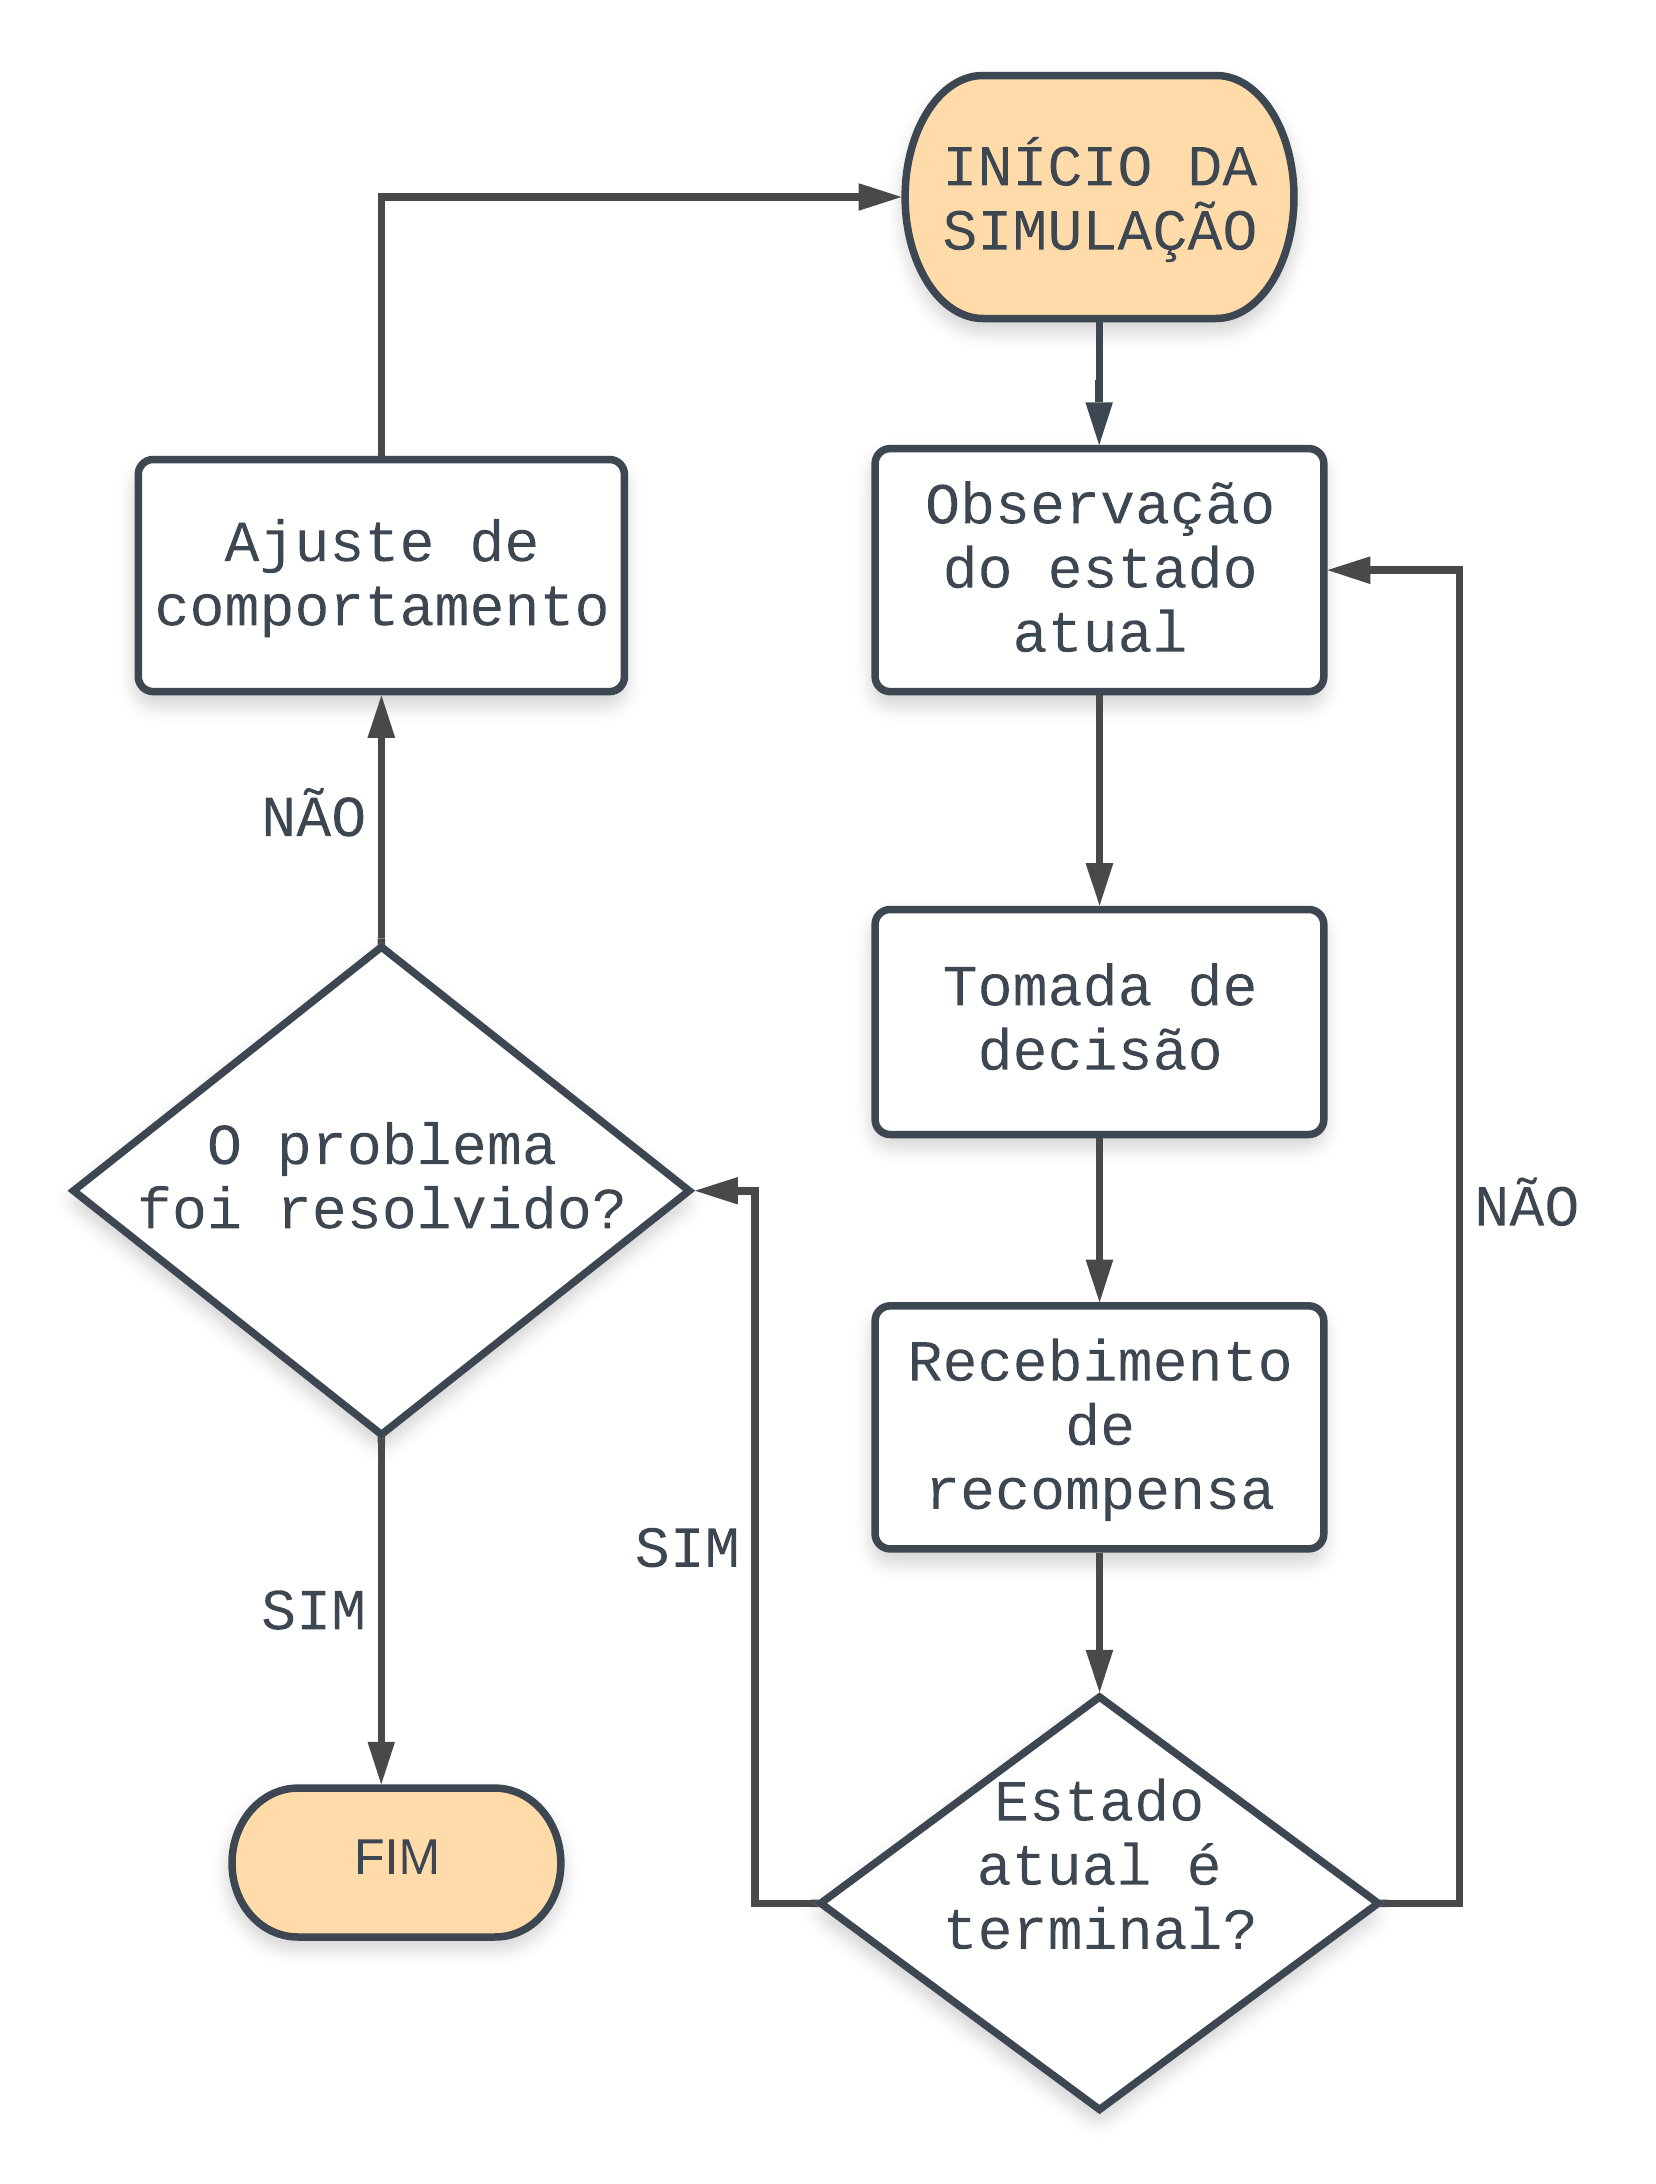
\includegraphics[width=0.65\textwidth]{fluxo_ar.png}
%     \end{center}
%     \label{fig:fluxo_ar}
% \end{figure}
%
%
% \subsection{Agente}
% Agente é a entidade dotada de capacidade de aprendizado que tenta extrair do ambiente a melhor maneira --- de acordo com uma
% métrica de performance, pré-estabelecida implicitamente via uma função de recompensa --- de executar uma determinada tarefa.
% No exemplo do gato de Thorndike, o agente é o próprio gato e
% as ações que ele executa são as possíveis interações com o interior da gaiola, a fim de abri-la. É o agente, portanto, a entidade responsável
% por decidir, através de uma observação do estado do ambiente, qual ação será tomada, visando sempre obter uma
% recompensa mais alta do que a maior recompensa recebida até o presente momento.
%
%
% Em alguns problemas, pode ser interessante que o estado do próprio agente seja lido antes que a próxima ação a ser tomada seja escolhida.
% Ou seja, pode ser relevante, a fim de determinar a melhor ação do agente, não apenas observar características do estado externo ao agente,
%  tais como a posição de diferentes obstáculos, mas também a observação de características do estado interno do agente, tal como seu nível atual de bateria
%  e o posicionamento físico das suas diferentes partes.
% Nesse caso, informações são coletas sobre todas as partes que formam o agente, tal como, por exemplo, a posição espacial de uma de
% suas pernas. No exemplo descrito na seção \ref{ambiente}, é imprescindível que o agente leve em consideração a posição do braço mecânico
% para decidir qual movimento será executado em seguida. Isso implica que a especificação do agente corresponde não apenas à descrição de seus
% componentes físicos, como no caso de um robô, mas também na definição de quais informações irão compor o estado com base no qual tal agente irá escolher ações;
% em particular, parte do estado pode envolver a observação de sensores internos ao próprio agente. Mais detalhes sobre isso serão discutidos
%  na Secao [secao onde fala de Estado].
%
%
% \subsection{Ambiente}
% \label{ambiente}
% O ambiente é o espaço onde o agente está inserido e de onde ele extrai as informações necessárias para decidir que ação será tomada.
% No ambiente podem se encontrar, por exemplo, objetos com os quais o agente deverá interagir para que o problema seja resolvido.
% Em um famoso problema de AR dentro do campo da robótica, um agente que simula um braço mecânico deve mover-se de tal maneira que
% sua extremidade esteja dentro de uma área demarcada no ambiente, área esta que é colocada em posições aleatórias ao início de cada episódio
% de treinamento (figura \ref{fig:roboticarm}). \par
%
% \begin{figure}[h]
%     \caption{Problema de aprendizado por reforço conhecido como \textit{Robotic Arm}.}
%     \begin{center}
%       \frame{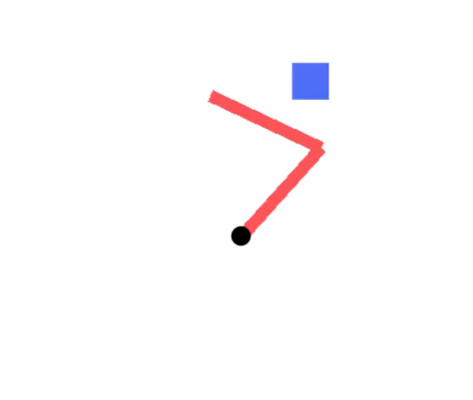
\includegraphics[width=0.65\textwidth]{roboticarm.png}}
%     \end{center}
%     \label{fig:roboticarm}
% \end{figure}
%
% Através de uma leitura da posição da área demarcada em azul, o agente deve decidir como irá ser executado o movimento do braço mecânico, composto
% de duas peças unidas, uma delas afixada no ponto de cor preta, no centro da tela, de modo a tocar a área azul com a extremidade do braço, fazendo
% sempre o mínimo possível de esforço, de forma a maximizar a recompensa (neste exemplo, a recompensa também toma como base a energia desprendida pelo
% braço mecânico para tocar a área demarcada). O ambiente compreende, por conseguinte, não só o espaço físico (real ou simulado) onde o agente está inserido e onde ele
% executa as suas ações; o ambiente é, além disso, a fonte de onde ele extrai as informações necessárias para decidir o que fazer,
% \bruno{e também contém a especificação da tarefa específica que o agente irá ter que resolver---e.g., mover o braço para uma posição específica, ou então empurrar um determinado objeto, etc}.
% \henrique{certeza que, filosoficamente falando, não é o agente que carrega a especificação do problema? na real, a especificação do problema é tratada no meu tcc como algo
% alheio ao agente e ao ambiente, ou seja, não pertencente a nenhum dos dois. acho que só serviria pra confundir ao invés de explicar que o ambiente de alguma maneira "carrega" consigo a definição do problema.
%  (tanto é que no meu trabalho a função que lê o estado e define se o problema já foi resolvido é separada dos dois)}
%
% \subsection{Estado}
% Estado, dentro de um contexto de AR, é o conjunto de informações referentes ao agente e ao ambiente em um determinado momento no tempo, e que é utilizado para calcular
% qual será a próxima ação a ser tomada pelo agente. Considerando que a tomada de ação do agente é regulada por uma função $\pi$ que mapeia um estado
% $s$ a uma ação $a$, o estado, nesse caso, é o subconjunto de todas as informações do agente e do ambiente que serão usadas em $s$.
%
%
% % \bruno{se depois tu vai falar de Q-Learning ou algo assim, é bom aqui começar a usar já a terminologia matemática padrão. A função que determina uma ação $a$ baseada no estado atual $s$ se chama uma política, e é normalmnete denotada por $\pi$. Ou seja, o agente escolhe ações usando uma função $\pi(s) \rightarrow a$. Depois de executar a ação escolhida, $a$, o agente observa o novo estado do ambiente,  $s'$, e recebe uma recompensa, $r$, e com base nisso atualiza a sua política $\pi$ de acordo com algum algoritmo de aprendizado. Não fala que ação é $t$, porque $t$ sugere tempo, nào ação. Muda no resto pra usar a notacao acima, que é a padrao, e que vai facilitar na hora de falar sobre q-learning. O que é importante dizer na secao atual é que pra que o agente consiga aprender de maneira efetiva, as informacoes que vao ser incluidas no estado $s$ precisam ser suficientes pra que contenham toda informacao necessaria para que o agente possa determinar a acao apropriada. E.g., num problema onde o agente precisa mover a mao para um determinado local, se o agente nao tiver dentro do seu estado a informacao sobre a posicao $x,y$ da sua mao no momento atual, ele nao tem uma parte essencial da informacao necessaria pra escolher a acao---e.g. se deve mover a mao para a direita ou para a esquerda}\par
%
% A definição desse subconjunto, ou seja, a determinação de quais informações das entidades envolvidas na tarefa de aprendizado irão compor o estado e serão
% levadas em conta para a próxima tomada de ação do agente, é de responsabilidade do desenvolvedor ou pesquisador que está construindo
% o agente. Em tarefas simples, como a do exemplo ilustrado pela figura \ref{robotichand}, é trivial a determinação de quais informações farão
% parte do estado: no exemplo, é óbvio que a posição da área em azul e das partes do braço mecânico serão levadas em conta. Em outros
% problemas, entretanto, onde há agentes mais complexos lidando com múltiplos objetos no ambiente, é menos óbvia a tarefa de determinar
% o conjunto $s$ que será fornecido como entrada à função $\pi$. Isto pode influenciar no tempo necessário para a conclusão de um projeto
% que envolva aprendizado por reforço, uma vez que vários conjuntos diferentes de informações devem ser testados de maneira iterativa
% até que seja encontrado um estado que minimize o tempo até a conclusão da tarefa e torne o agente mais capaz de resolver o problema.
%
%
% Estado, dentro de um contexto de aprendizado por reforço, portanto, é um subconjunto contido no conjunto de todas as possíveis informações oriundas
% de todos os elementos envolvidos dentro de uma tarefa de aprendizado  --- incluindo informações sobre o ambiente e sobre o próprio agente) --- e que é usado
% como entrada na função do agente que mapeia um estado $s$ a uma
% ação $a$. As informações que compõem o estado, entretanto, são fruto de uma decisão humana, por parte de quem está desenvolvendo o projeto, e,
% considerando que decisões diferentes podem trazer resultados diferentes (dependendo da complexidade do projeto), pode ser necessário
% que diferentes formas de compor o estado sejam testadas a fim de que se encontre qual delas é a mais satisfatória para o problema a ser resolvido.
%
% \subsection{Ação}
% Um agente de aprendizado por reforço deve, a cada momento tomar uma ação. Através da sua ação, o agente interage com o ambiente (e consigo mesmo)
% para provocar uma mudança no estado do sistema (e, conforme mencionado anteriormente, por estado do sistema compreende-se o estado tanto do agente quanto do ambiente
%  a fim de resolver
% o problema. Esta concepção de ação como uma interação com o ambiente que resulta em uma mudança no estado do sistema é inerente ao aprendizado por reforço:
% a grande diferença entre os diferentes algoritmos de AR, entretanto, reside em como a próxima ação é escolhida e em como o agente atualiza o seu comportamento,
%  baseado na observações sobre os resultados (e.g. recompensa recebida) após a execução da ação escolhida, para atualizar seu comportamento.
% %
% % FALAR SOBRE Q-LEARNING, POLICY LEARNING E MARKOV DECISION PROCESSES
% \bruno{mas nao falar de QL e essas outras coisas aqui, na secao que explica o que é Ação. Eu colocaria essas explicacoes em uma secao logo antes da 2.2, chamada algo como 'Formalizacao do Problema de Aprendizado e Algoritmos de AR'. Minha sugestao é começar falando que normalmente um problema de aprendizado por reforço é modelado como um MDP, o qual especifica o conjunto de estados possiveis, acoes possiveis, uma funcao de recompensa R que mapeia uma parte de estado atual e acao escolhida para um valor numerico de recompensa, uma funcao de transicao que determina, com no estado atual e acao escolhida, qual a probabilidade do sistema transicionar pra cada possivel estado seguinte, e um fator de desconto gamma. Ver no livro de IA (Russel and Norvig) a definicao direitinho. Diz que um MDP é a formalizacao matematica de como o ambiente funciona (via a funcao de transicao, cujo efeito é normalmente é implementado computacionalmente atraves de simuladores) e especficacao da tarefa a ser resolvida (via a função de recompensa). Aí diz que o objetivo é aprender uma política $\pi$ que, se usada pelo agente, maximize a soma de recompensas que ele recebe ao longo do episódio. Ver a definicao no livro. Diz que existem diferentes algoritmos para, com base nas interacoes do agente com seu ambiente, atualizar seu comportamnto/politica $\pi$. Um dos mais famosos é o Q-Learning. Aí explica o Q-L. Dá uma olhada nos slides de RL da aula de redes neurais que eu dei nesse semestre. Sao 3 pdfs, e se nao me engano tem definicoes la. A chave pra acessar/se cadsatrar o moodle da disciplina é 'rnsf\_20172'}
% %
% \subsection{Episódio}
%   Um episódio é, basicamente, uma fase de treinamento de um agente de aprendizado por reforço. A fase inicia com a criação do ambiente e a inserção
%   do agente nele (inicialização) e, após isso, o agente interage com o ambiente até que o estado do sistema seja um estado final. Em um problema que,
%   por sua complexidade, vem sendo usado como exemplo no uso de redes neurais profundas em treinamentos por aprendizado por reforço, um agente humanóide
%   precisa aprender a caminhar: um episódio termina, portanto, quando o agente cai no chão, quando não consegue superar algum obstáculo (figura \ref{fig:walkingrobot})
%   ou quando um determinado número de iterações é atingido.
%   \begin{figure}
%       \caption{Fim de um episódio: o agente não foi capaz de superar um obstáculo.}
%       \begin{center}
%         \frame{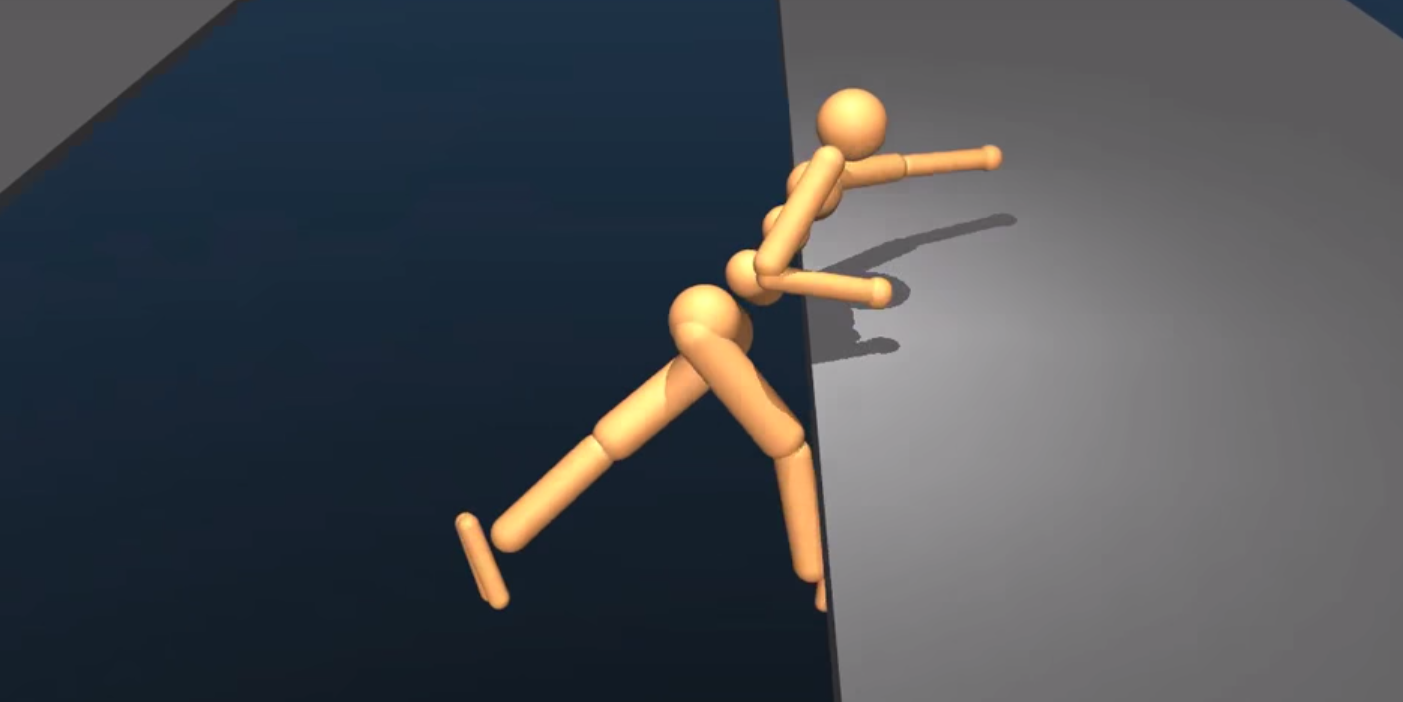
\includegraphics[width=0.65\textwidth]{walkingrobot.png}}
%       \end{center}
%       \label{fig:walkingrobot}
%   \end{figure}
%
% \subsection{Recompensa}
%
% Recompensa é um número atribuído a uma ação do agente que encapsula o sucesso desta quando o agente se encontra em um determinado estado. Para ações que
%  sejam avaliadas como melhores, a recompensa é mais alta;
% para ações que devem ser tratadas como indesejáveis pelo agente, a recompensa atribuída é mais baixa e, portanto, o agente deve corrigir-se a fim de que
% a ação que levou à baixa recompensa seja refinada ou abandonada de vez. É importante notar que nem sempre uma ação é diretamente ligada a uma recompensa:
% no caso de \textit{delayed reward}, a recompensa não é entregue ao agente no exato momento em que ele toma a decisão, sendo apenas revelada ao agente ao fim
% de uma sequência de ações. No caso de um
% agente que aprende a jogar damas, por exemplo, a recompensa é somente atribuída ao final da partida.
%
% \henrique{Isto leva a um problema bastante estudado no ramo
% do aprendizado por reforço chamado "atribuição de crédito": em uma série de ações que levaram a uma recompensa baixa, como encontrar, dentre todas as ações tomadas, apenas aquelas que
% foram responsáveis pelo baixo desempenho?  - eu nao sei onde tava querendo chegar quando escrevi isso e vou remover. azar}
%
% A recompensa é, portanto, um número que encapsula o quão adequada foi uma ação ou série de ações tomadas pelo agente para a resolução do problema. Para
% ações que tornam o agente mais próximo de resolvê-lo, é ideal que sejam recebidas recompensas mais altas. Para ações tidas como indesejáveis ou que não
% mudem o estado do sistema para um mais próximo do estado final, por outro lado, devem resultar em recompensas mais baixas para que o agente corrija seu
% comportamento.
%
% \section{Definição formal de um problema de aprendizado por reforço}
% O problema do aprendizado por reforço pode ser formalizado como um Processo de Decisão de Markov. Um Processo de Decisão de Markov representa um problema
% de aprendizado por reforço como uma constante troca de estados, onde cada troca representa uma ação e é seguida de uma recompensa. Cada estado, nesse caso,
% é uma observação do agente, e a transição é uma ação tomada por ele, que modifica o ambiente e leva a uma observação (ou seja, a outro estado) diferente.
% Um PDM modela uma função que procura maximizar o total de recompensas recebidas ao longo do tempo. A função é representada da seguinte maneira:
% \begin{equation}
%   \label{mdp}
%  \max{\sum_{t=0}^{t=\infty} \gamma^{t}r(s(t),a(t))}
% \end{equation}
%  Na fórmula, $r(s(t), a(t))$ é uma função que associa, em um instante de tempo $t$ uma recompensa $r$ a uma ação $a$ tomada quando o estado observado é
%  $s$. O objetivo da equação, portanto, é maximizar as recompensas recebidas ao longo do tempo tomando em cada momento a ação que leva à melhor recompensa.
%  O coeficiente $\gamma$, neste caso, é um número real no intervalo $(0,1]$ que determina a diferença de importância entre recompensas recebidas no presente
%  e no futuro.
%
% A fórmula \ref{mdp} capta de um modo geral o objetivo de um algoritmo de aprendizado por reforço: escolher, em um determinado instante de tempo, a ação que levará
% à maior recompensa. Porém, ainda falta definir como será escolhida a melhor ação $a$. Para isto, é necessário definir uma \textit{política}. Uma política
% pode ser representada como uma função $\pi(s) \rightarrow a$ que, recebendo um estado $s$, define que uma ação $a$ deve ser tomada. A fim de que, conforme
% definido na fórmula \ref{mdp}, sempre seja escolhida a melhor ação (i.e. a ação que leva a melhor recompensa), usa-se uma \textit{política ótima} $\pi*: S \rightarrow A$, que
% recebe um estado $s \in S$ e retorna uma ação ótima $a \in A$.
%
%
% Mesmo definindo matematicamente o problema de aprendizado por reforço em \ref{mdp} e definindo o que é uma política ótima, resta saber como encontrar uma
% política ótima. Em inteligência artificial, a noção de \textit{aprendizado} trata de uma correção que o agente executa em si mesmo, levando em consideração
% seu erro e um coeficiente de aprendizado, que determina o impacto que o último erro terá na atualização do agente em um determinado momento. Há muitos
% algoritmos de aprendizado por reforço que funcionam dessa maneira, e um dos mais estudados deles é chamado Q-learning.
%
% \section{Q-learning}
% \henrique{Coloco depois.}
% \blindtext
%
%
% \section{Simuladores de aprendizado por reforço}
% \begin{figure}[h]
%     \caption{Um robô real e sua versão modelada em um simulador.}
%     \begin{center}
%       \frame{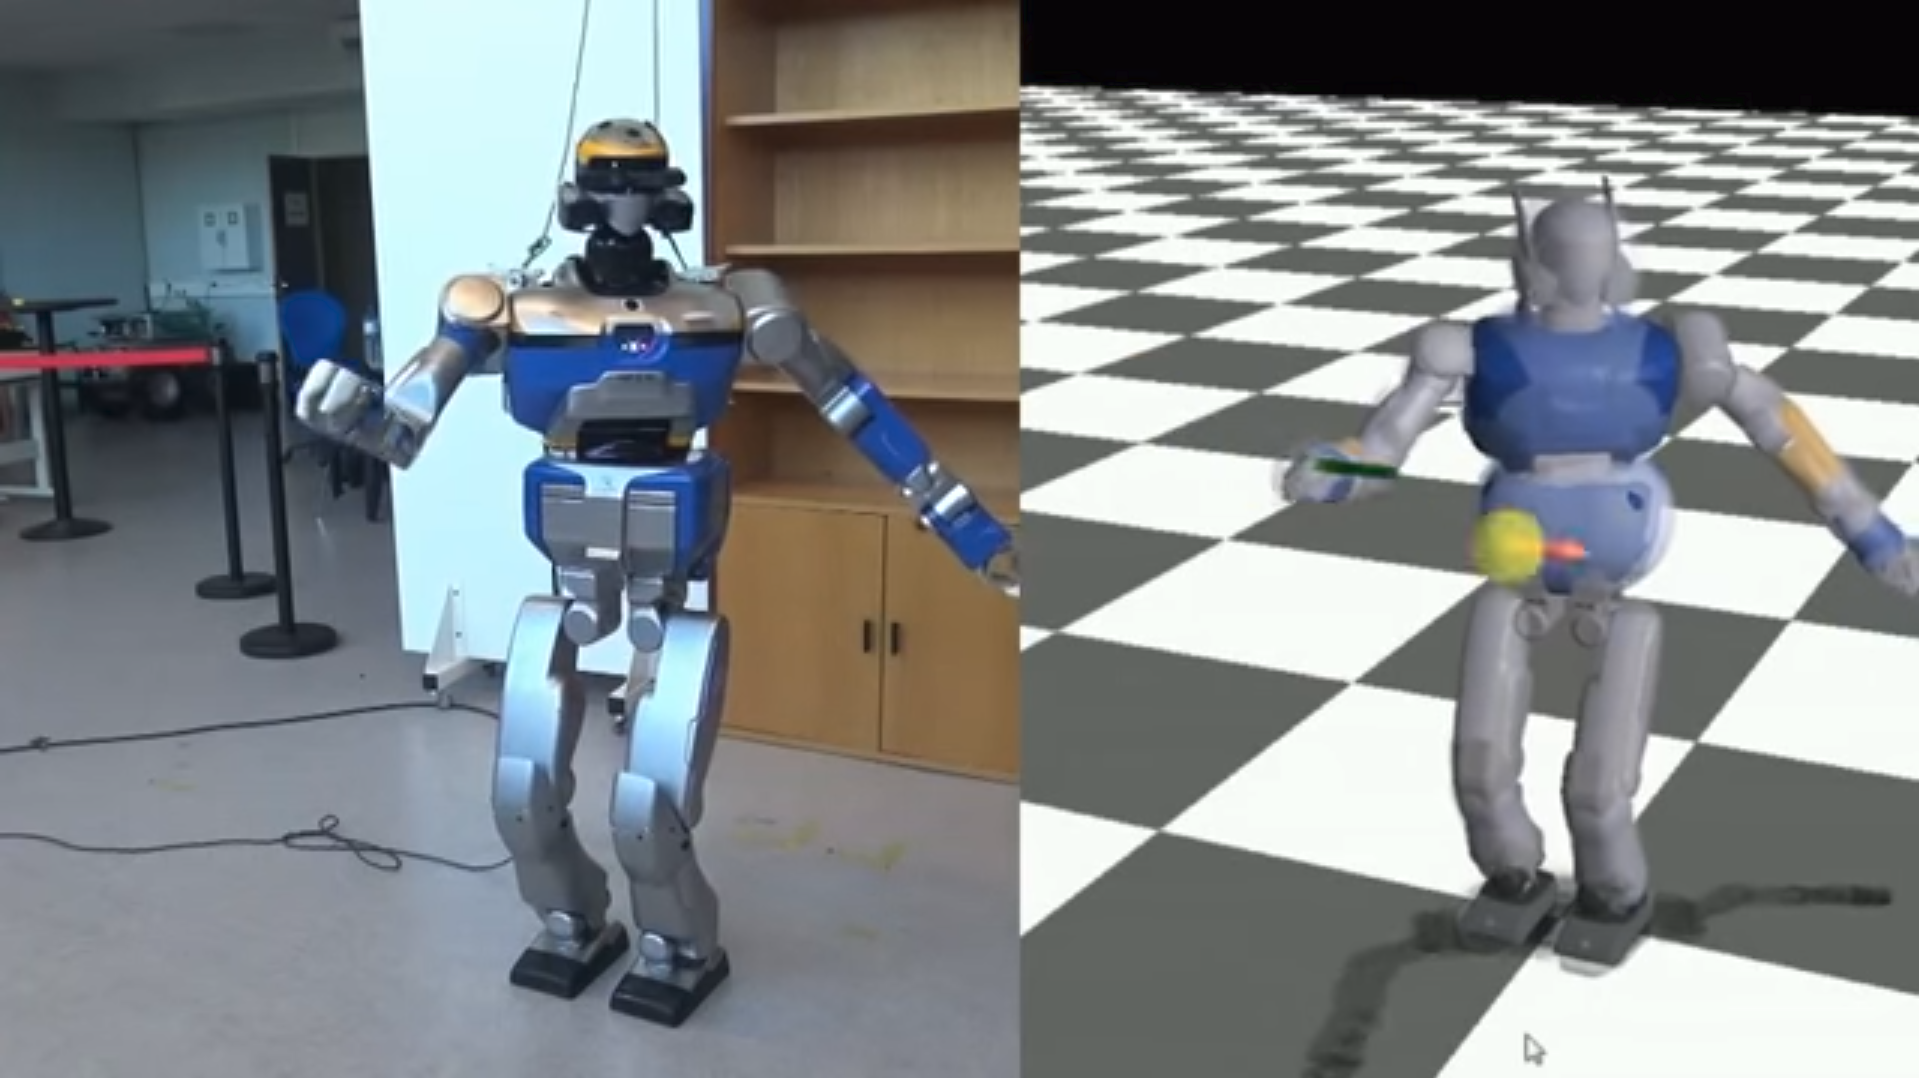
\includegraphics[width=0.9\textwidth]{mujocosimulator.png}}
%     \end{center}
%     \label{fig:mujocosimulator}
% \end{figure}
%
% Aprendizado por reforço lida com problemas onde um agente, inserido em um ambiente, tenta resolver um determinado problema através de uma série de ações.
% Em alguns problemas, é de interesse do responsável pelo desenvolvimento do agente que se possa modelar casos nos quais o agente está inserido em um ambiente
% %que desempenhe o papel de um sistema
% estocástico (i.e. que apresenta fatores aleatórios que influenciam em seu comportamento).
% No problema trabalhado na tese de Andrew Ng \bruno{add citation}, por exemplo, um agente é treinado para ser capaz de controlar um helicóptero, a fim de estabilizá-lo
% levando em consideração fatores imprevisíveis do sistema (e.g. vento, chuva e demais fatores que podem interferir na estabilidade do veículo).
% Nota-se que o problema, portanto, tem um objetivo prático: desenvolver um controle para um helicóptero que mantenha sua estabilidade, independentemente
% de fatores externos. O problema surge na necessidade de treinar o agente: como proceder com o treinamento em ambientes que possuam diferentes níveis
% de imprevisibilidade e cujos fatores como chuva e vento atuem em diferentes intensidades? Logicamente, o objetivo final do processo é ter um veículo
% autocontrolado capaz de manter sua estabilidade sob qualquer tipo de interpérie; para que isso seja possível, todavia, é necessário que o agente seja
% treinado em diferentes tipos de ambiente, o que pode se tornar inviável dadas restrições como o tempo disponível para o projeto e a necessidade dos
% desenvolvedores de se deslocar até locações onde há ambientes ideais para o treinamento. A solução que é amplamente usada nesses casos, portanto,
% é a modelagem de locações em um simulador que representa diferentes tipos de terreno e que permite ao pesquisador que este configure os diferentes
% fatores do ambiente de acordo com sua necessidade.
%
%
%
% Além da economia de tempo e da liberdade para modelar de forma controlada diferentes tipos de ambiente com comportamento estocástico, simuladores também oferecem uma maneira
% de analisar o desempenho de diferentes algoritmos de aprendizado quando aplicados ao mesmo problema, ou o contrário, que ocorre quando um mesmo algoritmo
% de aprendizado é aplicado a problemas diferentes a fim de que possa ser avaliada a sua generalidade. Esse foi um dos objetivos do desenvolvimento
% da plataforma Gym, da OpenAI, uma organização sem fins lucrativos que desenvolve projetos com foco em inteligência artificial.
% Com um catálogo de diversos cenários de aprendizado por reforço (chamados de \textit{environments}) oriundos da literatura de IA e até mesmo
% de jogos feitos para antigas plataformas de 8 \textit{bits}, esta plataforma oferece uma API (Interface Pública de Aplicação, em tradução livre; espécie
% de ponto de acesso ao qual programas podem se conectar, se seguirem um determinado formato) que permite que qualquer pessoa desenvolva seu algoritmo
% de AR para um determinado cenário e submeta-o a uma espécie de \textit{ranking}, que elenca os responsáveis pelos algoritmos que resolveram o problema de maneira mais eficiente,
% levando em consideração a maior recompensa recebida e o tempo levado para resolver o problema. Sua desvantagem, entretanto, é que o catálogo de \textit{environments}
% oferecido pelo Gym é fixo, ao mesmo tempo em que não existe nenhum \textit{framework} capaz de oferecer ao desenvolvedor as ferramentas necessárias
% para produzir cenários que são compativeis com a API do Gym. Isso possibilitaria, por exemplo, uma busca rápida de algoritmos que comprovadamente
% funcionam em cenários conhecidos a fim de que estes sejam mudados para sua aplicação em ambientes novos. Este trabalho propõe um \textit{framework}
% que auxilia na criação de tais cenários, sem que o programador tenha que lidar com questões de programação de baixo nível como a troca de informações
% entre um motor de física, responsável pelas simulações, e uma biblioteca gráfica, que transforma o ambiente simulado em algo que pode ser representado na
% tela através de \textit{pixels}.
% %
% %
% % \bruno{o Gym nao é um simulador, né? É uma API. Tu pode implementar diferentes ambientes, usando diferentes tipos de simuladores/motores de física, de forma que eles sejam compatíveis com Gym. O que eu diria aqui é que o Gym foi feito pra padronizar a interface com que algoritmos de AR interagem com diferentes ambientes simulados, independente de como tais ambientes simulados foram implementados---se manualmente, pelo programador usando diretamente um motor de fisica, ou usando algum dos framework para geracao de simulacoes/ambientes, tais como os que vao ser discutidos na secao de Estado da Arte. Como o Gym padroniza essa interface entre ambientes e agentes, quaisquer ambientes e  agentes/algoritmo de AR que sigam a API podem ser conectados, de forma a avaliar a performance daquele algoritmo naquele ambiente. Por essa razao, o Gym é um importante padrao na área pra facilitar essa comparacao de metodos, reproducibility, etc, aquelas coisas todas faladas no Resumo. Aí diz que, como sera discutido na secao de Estado da Arte, existem varios frameworks para facilitar a geracao de simulacoes/ambientes para avaliacao de algoritmos de AR, mas uma das limitacoes principais é que eles tem curva de aprendizado alta, etc, e que os codigos gerados automaticamente por esses frameworks nao seguem nenhuma interface padronizada, o que significa que é dificil pegar esses ambientes gerados e testar algoritmos implementados por outras pessoas, e disponibilizados online, nesses ambientes} Com um catálogo de
% % diversos problemas ou ambientes de aprendizado (chamados \textit{environments}) oriundos da literatura de IA e até mesmo de jogos que originalmente foram feitos para máquinas
% % de 8 bits, este simulador \bruno{gym nao é um simulador} permite que qualquer pessoa desenvolva seu algoritmo de AR e submeta-o a uma espécie de \textit{ranking}, que elenca os
% % responsáveis pelos algoritmos que resolveram o problema em menos tempo (i.e. que o agente aprendeu a sequência de ações que resolve o problema mais
% % rapidamente). Sua desvantagem, entretanto, é que os \textit{enviroments} são fixos e não permitem que neles sejam feitas pequenas alterações ou até
% % mesmo que \textit{environments} completamente novos sejam construídos, e este trabalho visa apresentar um simulador capaz de disponibilizar ferramentas
% % para a construção de cenários novos e que produzam resultados compatíveis com a biblioteca do Gym. \bruno{o final da frase (objetivo) ta ok, mas o inicio nao conecta bem: o teu trabalho nao é motivado pelo fato de que os codigos de ambientes do Gym nao fixos, porque tu nao vai propor um framework pra mais facilmente alterar codigos de ambientes do Gym. Tambem tem que corrigir onde tu diz que teu objetivo é fazer um simulador. É um framework pra gerar simualdores/ambientes etc etc}\par
%
%
% \henrique{aqui eu ainda tenho que alterar, com base no que vou colocar no capítulo de estado da arte}No próximo capítulo, será feito um breve estudo dos simuladores Gym e MuJoCo secao de traçando suas principais vantagens e deficiências, através de uma
% análise comparativa que relacionará seus pontos fortes e desvantagens com o que é oferecido pelo simulador descrito no capítulo 4 deste trabalho. \bruno{gym e mujoco sao comparaveis? gym é uma API, mujoco é um gerador de codigo. Tem que falar do Gym no inicio, clarificando que nao se trata de um simulador nem de um gerador de ambientes/simualdores, e sim um padrao/API que, se um deterinado ambiente/simulador seguir, ele pode ser usado para avaliar qualquer um dos N algoritmos de aprendizado que ja foram implementados e que seguem essa API. Aí precisa falar do mujoco e de outros geradores de codigo de ambientes/simuladores. Eu tinha mandado, num email, alguns links. Tem o framework dos italianos, e tinha um outro negocio que eu tinha mandado por facebook que era de um negocio meio em modo-texto. Nao lembro qual era. Mas tem mais coisa que só o mujoco; tem que achar os links que eu tinha mandado por email}.
%
% \section{A linguagem YAML}
% \label{alinguagemyaml}
% \henrique{Coloquei essa parte aqui porque faço referência a ela várias vezes durante o desenvolvimento.}
% YAML é uma linguagem de marcação utilizada para serialização de dados. Ela é usada normalmente para arquivos de configurações de sistemas (como é o caso do \textit{framework})
% Ruby on Rails, que permite a criação de servidores \textit{web} cujo acesso a seu banco de dados, por exemplo, é determinado por configurações salvas em um arquivo neste formato.
% Apesar de ter sido concebida como uma linguagem de marcação, pelo fato de sua sigla originalmente significar \textit{Yet Another Markup Language} ("mais uma linguagem de marcação", em tradução livre),
% mais tarde sua sigla se tornou recursiva e seu significado mudou para \textit{YAML: YAML Ain't Markup Language} ("YAML não é linguagem de marcação"),
% como forma de reposicionamento por parte seus desenvolvedores, que buscavam redirecionar o uso da linguagem para representações de dados, uso este que é
% bem diverso de marcação de texto. \par
% Sua sintaxe permite a declaração de vetores associativos (também conhecidos como "dicionários"), onde valores são associados a chaves, sendo estas normalmente
%  de caracteres.
% A possibilidade de definir dicionários, juntamente com a capacidade da linguagem de estruturar dados sob a forma de listas, permite que o programador defina
% estruturas bastante complexas, mas que são sintaticamente mais simples do que se os mesmos dados fossem definidos usando-se de outras linguagens de marcação, como XML e JSON.
%
% % http://ieeexplore.ieee.org/abstract/document/6215346/
%
% % (retirado de docs.ansible.com/ansible/latest/YAMLSyntax.html)
%
% Um exemplo do uso da linguagem YAML é dado abaixo. Nele, define-se uma lista composta de dois
% funcionários que possuem informações como nome, posição e uma lista de habilidades.
%
% \begin{minted}{yaml}
%   # Employee records
% -  martin:
%     name: Martin D'vloper
%     job: Developer
%     skills:
%       - python
%       - perl
%       - pascal
% -  tabitha:
%     name: Tabitha Bitumen
%     job: Developer
%     skills:
%       - lisp
%       - fortran
%       - erlang
% \end{minted}
%
%
% A ferramenta de modelagem de cenários de aprendizado por reforço descrita neste trabalho oferece duas maneiras de modelagem de entidades de AR e uma delas
% funciona através da leitura de um \textit{script} YAML que descreve, de maneira hierárquica, as entidades e suas propriedades. Uma descrição detalhada de como
% descrever um problema de AR através de um arquivo YAML é dada no capítulo 5 deste documento.
% er um problema de AR através de um arquivo YAML é dada no capítulo 5 deste documento.

\chapter{Estado da Arte}


No capítulo anterior, foi apresentada a formulação matemática de um problema de
AR e discutiu-se a respeito de simuladores de aprendizado por reforço, onde
discorreu-se sobre as vantagens de usar simuladores em problemas práticos bem
como na estrutura comum que é compartilhada por todos os simuladores de AR.
Neste capítulo, serão apresentadas diferentes maneiras de se construir um
simulador que representa um problema a ser resolvido por um agente de AR.
Alguns recursos que podem ajudar no processo, como motores de física, serão
apresentadas e, ao final do capítulo, será proposta uma hierarquia na qual as
diferentes ferramentas se organizam de acordo com o seu grau de especificidade.

\section{Construindo um simulador de aprendizado do zero}

Como qualquer outro problema do universo da ciência da computação, é possível
construir um simulador de aprendizado por reforço a partir dos elementos básicos
de entrada, processamento e saída de dados fornecidos por linguagens de
programação como \textit{Python} e C++. Tomemos como exemplo um problema onde um
agente é responsável por copiar uma sequência genética. No problema, para uma
sequência de $n$ genes, o agente recebe $1$ como recompensa para um gene copiado
corretamente e $0$ para genes copiados incorretamente. Construir uma simulação
deste problema é bastante simples: basta que seja usada uma sequência de
caracteres para representar os genes. O código referente ao
problema está listado no código-fonte \ref{dna}. No código, é possível perceber
que nenhuma ferramenta além daquelas que são oferecidas pelo pacote básico da
linguagem \textit{Python} é utilizada: um gerador de números inteiros, oferecido
nativamente pela linguagem, é o mecanismo mais complexo colocado em uso. A
estrutura de aprendizado por reforço e o ciclo da figura \ref{fig:fluxo_ar} também
estão bastante claros no código.

\begin{longlisting}
\begin{minted}{python}
from random import randint

MIN_SIZE = 10
MAX_SIZE = 100
EPISODES = 2
GENES = ['G', 'C', 'A', 'T']

# definição do problema
class DNACopy():
    def __init__(self):
        self.init()

    # inicialização
    def init(self):
        self.i = 0
        self.sequence = []
        self.copy = []
        size =
        for i in range(randint(MIN_SIZE, MAX_SIZE)):
            self.sequence.append(GENES[randint(0, 3)])
        return self.sequence[i]
    def size(self):
        return len(self.sequence)

    # método de tomada de ação
    def action(self, g):
        self.copy.append(GENES[g])
        self.i += 1
        return self.reward(g)

    # método de observação
    def observation(self):
        return self.sequence[self.i]

    # método de cálculo de recompensa
    def reward(self, g):
        return int(self.sequence[self.i] == \
         GENES[g])

for e in range(EPISODES):
    problem = DNACopy()

    # inicialização do problema e da recompensa
    problem.init()
    reward = 0

    # ciclo de tomada de ações
    for action in range(problem.size() - 1):
        # ação aleatória é tomada e
        # a recompensa é somada à variavel reward
        a = random.randint(0, len(GENES) - 1)
        reward += problem.action(a)
    print("Total reward is %d" % reward)

\end{minted}
\caption[Cópia de DNA]{Exemplo de um problema de cópia de material genético.}
\label{dna}
\end{longlisting}

O problema é bastante simples: para um material genético de tamanho $m$, a
recompensa total recebida é $n/m$, onde $n$ é o número de genes copiados
corretamente. Mas e para problemas mais complexos, que envolvem não sequências
de caracteres que representam genes, mas objetos localizados em um espaço de
duas ou três dimensões, como representar os elementos do problema nativamente?
Problemas mais complexos requerem, naturalmente, o uso de ferramentas mais
complexas para sua construção e motores de física, ferramentas capazes de
representar objetos no espaço e de simular as o contato entre eles, são um belo
exemplo disso.
Vejamos o exemplo do ramo da robótica, por exemplo. Qualquer tarefa que necessite
ser executada repetidamente e com certo grau de precisão é uma boa candidata
para a automatização através do emprego de robôs: linhas de montagem de
empresas automotivas, por exemplo, já são dominadas por robôs há varios anos.
Outras tarefas, mais complexas do que as executadas pelos robôs da manufatura,
mas ainda assim consideradas maçantes e repetitivas por humanos --- como
dirigir, por exemplo ---, também são fortes candidatas à automação, tendo, nos
últimos tempos, sido alvo de pesquisas de ponta envolvendo inteligência
artificial, com a popularização de técnicas de aprendizado de máquina e visão
computacional. É aí que entra o uso de simuladores: durante as fases iniciais
de desenvolvimento de um robô, uma versão virtual deste pode ser construída,
como na figura \ref{fig:mujoco_robot}, em um ambiente fundamentado em motores
de física que simulam as leis do mundo real. No ambiente controlado de um
simulador, o treinamento do agente pode ser feito de forma acelerada, fazendo
com que as primeiras versões reais do robô já apresentem uma versão incial do
comportamento que quer-se ensinar a ele.
A construção de motores de física que executam cálculos que simulam a interação
entre objetos em espaços multidimensionais faz parte de um amplo campo de
pesquisa e desenvolvimento, então é natural que seja desnecessário para quem
está desenvolvendo um simulador de aprendizado por reforço implementar um novo
motor do zero.


\section{Motores de Física}
Um motor de física nada mais é do que um programa que simula leis de Newton
utilizando princípios como massa, velocidade, atrito e resistência do ar,
tornando possível a modelagem de situações que envolvem a física do mundo real.
Muito utilizados nos campos de pesquisa e de jogos eletrônicos, motores de
física são essenciais para garantir a verossimilhança de uma simulação de um
problema de robótica ou de um jogo, por exemplo.


Robôs executam tarefas através do contato físico com o ambiente que os cerca. É
primordial, portanto, para o desenvolvimento do \textit{software} que compõe o
robô, que existam ferramentas capazes de reconstruir, com elevado grau de
precisão, em um ambiente virtual e controlado, os aspectos físicos de todos os
elementos que podem estar à sua volta. Para isso, um simulador deve definir os
corpos no espaço e calcular as forças resultantes do contato entre eles, o que é
um problema NP-difícil \cite{Kaufman2008}. Para tratar o problema, motores de
física utilizam de versões relaxadas do problema, permitindo que este seja
tratado por métodos de solução que envolvem programação linear.


A ideia por trás de um motor de física é simples:  define-se um intervalo de
tempo $\delta$ e, para um instante de tempo $t$, todas as interações entre os
objetos representados e as resultantes das forças neles aplicadas são
calculadas, e o resultado destes cálculos são as posições dos objetos e as
forças que sobre eles atuam no instante de tempo $t+\delta$. Imprecisões são
proporcionais a $\delta$, ou seja, um simulador de física só é completamente
preciso se o intervalo $\delta$ é infinitamente pequeno.


Em um mundo ideal, simulações feitas por um motor de física teriam ao mesmo
tempo um custo computacional pequeno e uma precisão próxima da realidade. O que
acontece, entretanto, é uma espécie de \textit{trade-off} entre a precisão da
simulação e o tempo necessário para sua execução: em aplicações onde o mais
importante é a velocidade da simulação, como em jogos eletrônicos --- onde o
$\delta$ é normalmente $\frac{1}{60}s$ --- o sistema pode abrir mão da precisão.
Em simulações utilizadas na robótica, por outro lado, a precisão é muito mais
importante, uma vez que a simulação pode anteceder um experimento feito no
mundo real e imprecisões no motor de física podem levar a resultados
completamente divergentes da realidade. Conforme apontado em \cite{Sims1994},
imprecisões em simulações serão invariavelmente exploradas por algoritmos de
otimização.


Todas estas nuances devem ser levadas em consideração na hora de se escolher ou
desenvolver um motor de física, o que torna complicada a tarefa de decidir qual
será a ferramenta utilizada para a simulação que se deseja desenvolver.
Desenvolver um motor de física próprio, entretanto, é uma tarefa ainda mais
complexa. O mero cálculo de forças que atuam sobre corpos unidos por juntas, por
exemplo, pode requerer o uso de diversas fórmulas \cite{ODEJoints2002}. Para
aqueles que desejam desenvolver aplicações de aprendizado por reforço, portanto,
surge a necessidade de se estudar diferentes ferramentas de física, o que pode
consumir bastante tempo.


Há vários motores de física disponíveis, alguns com custo e outros sob licenças
de código aberto. Os mais frequentemente utilizados, bem como exemplos de
aplicações de aprendizado por reforço onde eles são empregados, são apresentados
a seguir. Alguns dos motores apresentados fornecem simulações
robustas, porém mais lentas; outros, por sua vez, por serem voltados à
aplicações visuais, realizam as simulações mais rapidamente, mas com perda de
precisão. Foram trazidos para este trabalho três motores de física bastante
conhecidos, sendo dois deles tridimensionais e um bidimensional. Além disso,
este trabalho descreve também um estudo \cite{LeggedRobotics2018}, que compara não
só os dois motores de física tridimensionais apresentados nesta seção, como dois
outros simuladores de propósito mais específico, apresentados na seção seguinte.


O trabalho desenvolvido em \cite{LeggedRobotics2018} apresenta um estudo
comparativo entre diversos motores de física onde cada um dos cenários de teste
verifica o comportamento de uma característica diferente das  simulações. São
sete cenários de teste ao todo:


\begin{itemize}
  \item \textit{Rolling test}: teste de modelos de fricção. Testa a capacidade
  dos motores de simular forças de atrito corretamente;
  \item \textit{Bouncing test}: nesta simulação um objeto esférico cai no chão.
  Testa a capacidade dos motores de simular forças de colisão elástica;
  \item \textit{666 balls test}: uma perturbação é inserida em uma pilha de
  tamanho $6 \times 6 \times 6$ de objetos esféricos. Testa a capacidade dos
  motores de lidar com colisões sólidas envolvendo múltiplos corpos;
  \item \textit{Elastic 666 balls test}: mesma situação que o cenário anterior,
  porém com colisões elásticas;
  \item \textit{ANYmal PD control test}: neste cenário, um robô quadrúpede
  \cite{ANYmal} deve permanecer em pé. O cenário testa a precisão da
  representação das juntas e a escalabilidade do motor, uma vez que o teste é
  repetido várias vezes para um número crescente de robôs;
  \item \textit{ANYmal momentum test}: neste cenário, um objeto esférico colide
  com o robô. É testada a capacidade do motor de representar as juntas
  corretamente durante e após o momento da colisão;
  \item \textit{ANYmal energy test}: neste cenário, o robô é objeto de uma força
  que o impulsiona para cima. O cenário testa a capacidade do motor de
  representar as juntas do robô corretamente durante a queda e no instante que
  ele colide com o chão.

\end{itemize}


\subsubsection{Open Dynamics Engine}

Sendo uma ferramenta de simulações físicas de propósitos gerais, a
\textit{Open Dynamics Engine} \cite{ODE} foi feita para simular propriedades
físicas de corpos articulados. Este motor é ideal para simulações que possam
envolver veículos ou criaturas bípedes, por exemplo. Com uma extensa biblioteca
capas de gerar fidedignas dos mais variados corpos tridimensionais e de junções
que os conectam, a ODE vem sendo mantida por mais de uma década, contando com
uma comunidade bastante ativa de desenvolvedores. Entretanto, justamente por
ser um motor de física relativamente antigo, a \text{ODE} acaba por não se
beneficiar de tecnologias mais recentes, como paralelismo, por exemplo. Há
registros de tentativas de expansão da ferramenta para adicionar o suporte a
processamento paralelo, mas a tarefa se provou desafiadora \cite{ODEParallel}.

Na avaliação conduzida em \cite{LeggedRobotics2018} a \textit{ODE} se destaca no
cenário \textit{ANYmal momentum test}, saindo-se ligeiramente melhor, no que se
refere à acurácia da simulação (neste cenário, o erro é representado pela
diferença quadrática entre a quantidade de energia que deveria haver no sistema
em uma simulação ideal e a quantidade de energia presente no sistema simulado,
medido em $(N \cdot m/s)^2$). Deve ser observado, entretanto, que, mesmo no
cenário de teste em que a \textit{Open Dynamics Engine} apresentou simulações de
qualidade, o tempo utilizado pelo motor para computar as simulações é muito
maior do que o tempo usado nos outros motores, o que se deve pelo fato da
\textit{ODE} ser um sistema antigo, e que portanto não se beneficia de
ferramentas de paralelização fornecidas por processadores recentes.


Ainda assim, a \textit{ODE} é amplamente utilizada em jogos, talvez pelo fato de
ser um sistema de código aberto, licenciado sob a BSD e a LGPL, e também em
razão do sistema ter sido portado para diversas linguagens de programação
diferentes. Abaixo, um exemplo de código que utiliza a versão em \textit{Python}
da \textit{ODE} para, juntamente com a biblioteca \textit{Pygame}, desenhar um
pêndulo.

\begin{longlisting}
\begin{minted}{python}
# pyODE example 2: Connecting bodies with joints

import pygame
from pygame.locals import *
import ode


def coord(x,y):
    "Convert world coordinates to pixel coordinates."
    return 320+170*x, 400-170*y


# Initialize pygame
pygame.init()

# Open a display
srf = pygame.display.set_mode((640,480))

# Create a world object
world = ode.World()
world.setGravity((0,-9.81,0))

# Create two bodies
body1 = ode.Body(world)
M = ode.Mass()
M.setSphere(2500, 0.05)
body1.setMass(M)
body1.setPosition((1,2,0))

body2 = ode.Body(world)
M = ode.Mass()
M.setSphere(2500, 0.05)
body2.setMass(M)
body2.setPosition((2,2,0))

# Connect body1 with the static environment
j1 = ode.BallJoint(world)
j1.attach(body1, ode.environment)
j1.setAnchor( (0,2,0) )

# Connect body2 with body1
j2 = ode.BallJoint(world)
j2.attach(body1, body2)
j2.setAnchor( (1,2,0) )


# Simulation loop...
fps = 50
dt = 1.0/fps
loopFlag = True
clk = pygame.time.Clock()

while loopFlag:
    events = pygame.event.get()
    for e in events:
        if e.type==QUIT:
            loopFlag=False
        if e.type==KEYDOWN:
            loopFlag=False

    # Clear the screen
    srf.fill((255,255,255))

    # Draw the two bodies
    x1,y1,z1 = body1.getPosition()
    x2,y2,z2 = body2.getPosition()
    pygame.draw.circle(srf, (55,0,200),\
      coord(x1,y1), 20, 0)
    pygame.draw.line(srf, (55,0,200),\
      coord(0,2), coord(x1,y1), 2)
    pygame.draw.circle(srf, (55,0,200),\
      coord(x2,y2), 20, 0)
    pygame.draw.line(srf, (55,0,200),\
      coord(x1,y1), coord(x2,y2), 2)

    pygame.display.flip()

    # Next simulation step
    world.step(dt)

    # Try to keep the specified framerate
    clk.tick(fps)
\end{minted}
\caption[]{Exemplo de uma simulação que usa a Open Dynamics Engine.}
\label{ode_example}
\end{longlisting}

% daqui http://pyode.sourceforge.net/tutorials/tutorial2.html

É necessário observar no código acima que as chamadas da função que atualiza as
propriedades físicas de cada objeto depois de um intervalo $dt$ e da função que
desenha os objetos criados não é automática, sendo de responsabilidade do
programador. No capítulo seguinte deste trabalho, será exposto como a ferramenta
proposta tenta simplificar estas tarefas.

\subsubsection{Bullet Physics}
% [[1]] https://bulletphysics.org
% [[2]] https://xbpeng.github.io/projects/DeepMimic/2018_TOG_DeepMimic.pdf
% [[3]] https://arxiv.org/pdf/1903.11239.pdf
% [[4]] https://xbpeng.github.io/projects/DeepMimic/index.html


O motor de física \textit{Bullet Physics} \cite{BulletPhysics} tinha como
propósito principal ser usado para jogos eletrônicos, tendo também sido usado
na criação de efeitos especiais em filmes. Quanto à sua performance, a
ferramenta apresenta um comportamento parecido com a \textit{ODE}, com a
diferença de que a \textit{Bullet} apresenta um grau de sofisticação maior em
simulações que devem levar forças de fricção em consideração, executando as
simulações relacionadas a esta força de maneira eficiente e acurada e, portanto,
apresentando um desempenho melhor nos cenários relacionados em \cite{LeggedRobotics2018}.
Assim como a \textit{ODE}, a biblioteca \textit{Bullet} apresenta um desempenho melhor
quando o objeto representado é representado por apenas um corpo, formado por uma
das primitivas (i.e. unidades básicas de construção) da ferramenta, enquanto o
\textit{MuJoCo}, por exemplo, se comporta melhor quando a simulação envolve
corpos complexos.

\begin{figure}[h]
    \caption{TossingBot}
    \begin{center}
      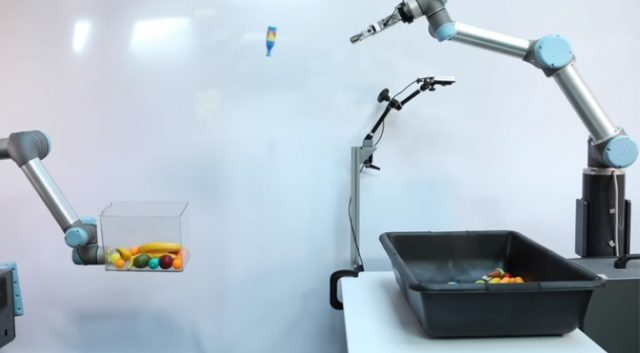
\includegraphics[width=0.9\textwidth]{tossingbot.jpg}
    \end{center}
    \label{fig:tossingbot}
\end{figure}


Dois trabalhos construídos com a ajuda da \textit{Bullet Physics} merecem
atenção: em um deles, um robô formado por um braço e um par de pinças, com uma
caixa cheia de objetos disposta à sua frente, deve inferir, a partir de
informações visuais, como pegar objetos de dentro da caixa e arremessá-los em
uma outra caixa, disposta um pouco mais distante (figura \ref{fig:tossingbot}).
O treinamento do robô, chamado de \textit{TossingBot} \cite{TossingBot2019}, envolveu uma simulação
utilizando-se da \textit{Bullet Physics}. É importante notar a natureza da
simulação, que envolveu uma série de corpos (no caso, os objetos da caixa) sem
nenhum tipo de conexão entre si, cenário para o qual este motor de física é
recomendado. Em outro trabalho \cite{DeepMimic}, um agente deve analisar imagens de atores,
captadas por câmeras ou por ferramentas de \textit{motion capture}, e fazer com
que um robô, simulado em um ambiente que usa a biblioteca \textit{Bullet},
imite os movimentos ou desenvolva variações deles.

\textit{Bullet} apresentou boa performance nos cenários de teste apresentados
em \cite{LeggedRobotics2018} e, além disso, conta com diversas bibliotecas que a integram a várias
linguagens de programação, como \textit{Python}, por exemplo. Esta combinação de
praticidade e boa performance é, provavelmente, um dos motivos que fez com que
os desenvolvedores do simulador \textit{Gazebo} tenham adotado \textit{Bullet}
como um dos motores de física que compõem a base das simulações da ferramenta.


\subsubsection{Box2D}

% http://eprints.lincoln.ac.uk/28089/1/LearningToAssembleObjectsWithARobotSwarm.pdf

Há situações em que um motor de física tridimensional é desnecessário. Em jogos
eletrônicos, por exemplo, quando, por uma opção de \textit{design}, o jogo é
desenvolvido em um ambiente bidimensional, não há a necessidade de usar motores
que usem mais do que duas dimensões para representar seus objetos. O grau de
complexidade de motores bidimensionais, entretanto, é praticamente o mesmo de
motores de três dimensões, uma vez que o problema de simular interações físicas
em ambientes bidimensionais também deve ser tratado de maneira aproximada,
fazendo com que motores do tipo apresentem o mesmo \textit{trade-off} entre
custo computacional e acurácia.


De todos os motores bidimensionais, talvez o mais conhecido seja o \textit{Box2D}
\cite{Box2d}. Criado para o desenvolvimento de jogos, a ferramenta possui
versões para diversas linguagens de programação diferentes. O trecho de código
a seguir visa evidenciar as semelhanças entre um programa que utiliza Box2D e o
código-fonte \ref{ode_example}, que utiliza Open Dynamics Engine. Em ambos, o
a função que atualiza as propriedades físicas de cada objeto deve ser chamada
e um instante de tempo deve ser fornecido.

\begin{minted}{c++}
for (int32 i = 0; i < 60; ++i)
{
 world.Step(timeStep, velocityIterations, positionIterations);
 b2Vec2 position = body->GetPosition();
 float32 angle = body->GetAngle();
 printf("%4.2f %4.2f %4.2f\n", position.x, position.y, angle);
}
\end{minted}

\noindent\makebox[\linewidth]{\rule{\paperwidth}{0.4pt}}


Um exemplo de pesquisa que utiliza Box2D pode ser encontrada em \cite{Box2DExample}.
Neste trabalho, um enxame de robôs, simulado no ambiente da ferramenta, deve
aprender a resolver tarefas em conjunto.

\section{Simuladores de propósito específico}
\blindtext

\subsection{DART}
Voltado, assim como o \textit{MuJoCo}, para simulações envolvendo robótica,
a ferramenta chamada \textit{DART} (de \textit{Dynamie Animation and Robotics
Toolkit}) foi desenvolvida em 2012. Nos testes apresentados em [[1]], apresentou
um comportamento regular, exceto no teste de fricção, onde os objetos simulados
não se comportaram da maneira esperada.

Em todos os cenários de teste, \textit{DART} apresentou o pior desempenho em
todos eles, apresentando imprecisões grotescas no cenário que envolve fricção.
Apesar de não possuir um desempenho excepcional, entretanto, \textit{DART} foi
adotada como
um dos motores de física que formam a base do simulador \textit{Gazebo}, voltado
especialmente para a robótica. O simulador é capaz de importar arquivos que,
utilizando uma sintaxe própria, definem robôs e criá-los no ambiente simulado de
uma maneira relativamente simples. Mais sobre o \textit{Gazebo} na seção
\ref{gazebo}.


\subsection{Gazebo}
% [[1]] http://citeseerx.ist.psu.edu/viewdoc/download?doi=10.1.1.304.8999&rep=rep1&type=pdf
% [[2]] https://www.willowgarage.com/sites/default/files/icraoss09-ROS.pdf

\textit{Gazebo} [[1]] é uma ferramenta voltada para a simulação de cenários envolvendo
problemas de robótica. Dotada de uma interface gráfica que auxilia na criação
de ambientes tridimensionais e dos robôs nele inseridos, \textit{Gazebo}
facilita enormemente o trabalho de pesquisadores e desenvolvedores da área de
robótica, uma vez que fornece meios de definir robôs e ambientes através de uma
linguagem própria de marcação, o que não só simplifica o trabalho de
desenvolvimento, mas também estimula o compartilhamento de diferentes modelos
entre os membros da comunidade.


\textit{Gazebo} é compatível com um sistema chamado \textit{ROS} [[2]] --- de
\textit{Robot Operating System}, ou Sistema Operacional de Robôs, em tradução
livre ---, que agrupa uma série de bibliotecas, ferramentas e convenções que
visam não apenas simplificar a tarefa de desenvolver um robô, mas também de
estabelecer normas e padrões a fim de que seja facilitada e estimulada a
colaboração entre pesquisadores de diversas instituições. Assim como no
\textit{software} fornecido pelo \textit{Gazebo}, \textit{ROS} também fornece
uma linguagem própria de marcação pela qual é possível definir robôs e o espaço
no qual eles estão inseridos. O formato também é compreendido pelo
\textit{Gazebo}, simplificando o intercâmbio de informações entre os dois
sistemas.


Conforme descrito em [[1]], \textit{Gazebo} oferece um meio de integrar
descrições textuais de alto nível de robôs e de ambientes com diferentes motores
de física, incluindo \textit{Bullet Physics}, \textit{DART} e \textit{ODE}, com
\textit{ODE} sendo o padrão, podendo ser facilmente substituído. Esta é a grande
vantagem oferecida por \textit{Gazebo} àqueles que decidem adotar seu
\textit{software}: é oferecido aos desenvolvedores e pesquisadores um ambiente
rico e agnóstico quanto às ferramentas utilizadas, uma vez que vários sistemas
amplamente usados são compatíveis com \textit{Gazebo}. Além disso, o
\textit{software} não tem custo e seu código é aberto, o que sifnifica que ele
pode ser alterado e qualquer pessoa pode contribuir com mudanças e adições nele.
Isto possibilitou que florescesse uma comunidade bastante ativa de pessoas
dispostas a contribuir com o projeto, desenvolvendo modelos de robôs e ambientes
com o objetivo de compartilhá-los. Todo o material já produzido pela comunidade,
aliado às ferramentas que o \textit{software} disponibiliza para a rápida
criação de modelos e ambientes, é o que faz o \textit{Gazebo} ser o que é. Seu
uso é tão simples que ele é utilizado até por alunos de graduação, inclusive
na UFRGS.

\subsection{MuJoCo}
% [1] https://ieeexplore.ieee.org/abstract/document/6386109
% [2] controller optimization => https://arxiv.org/abs/1509.01066
% [3] http://proceedings.mlr.press/v48/mniha16.pdf
% [4] https://arxiv.org/pdf/1707.02286.pdf
% [5] http://people.reed.edu/~jimfix/math385/lec01.1/Animation/p15-sims-evolving.pdf

\label{mujoco}

\begin{figure}[h]
    \caption{Modelagem de robôs humanoides no ambiente do MuJoCo}
    \begin{center}
      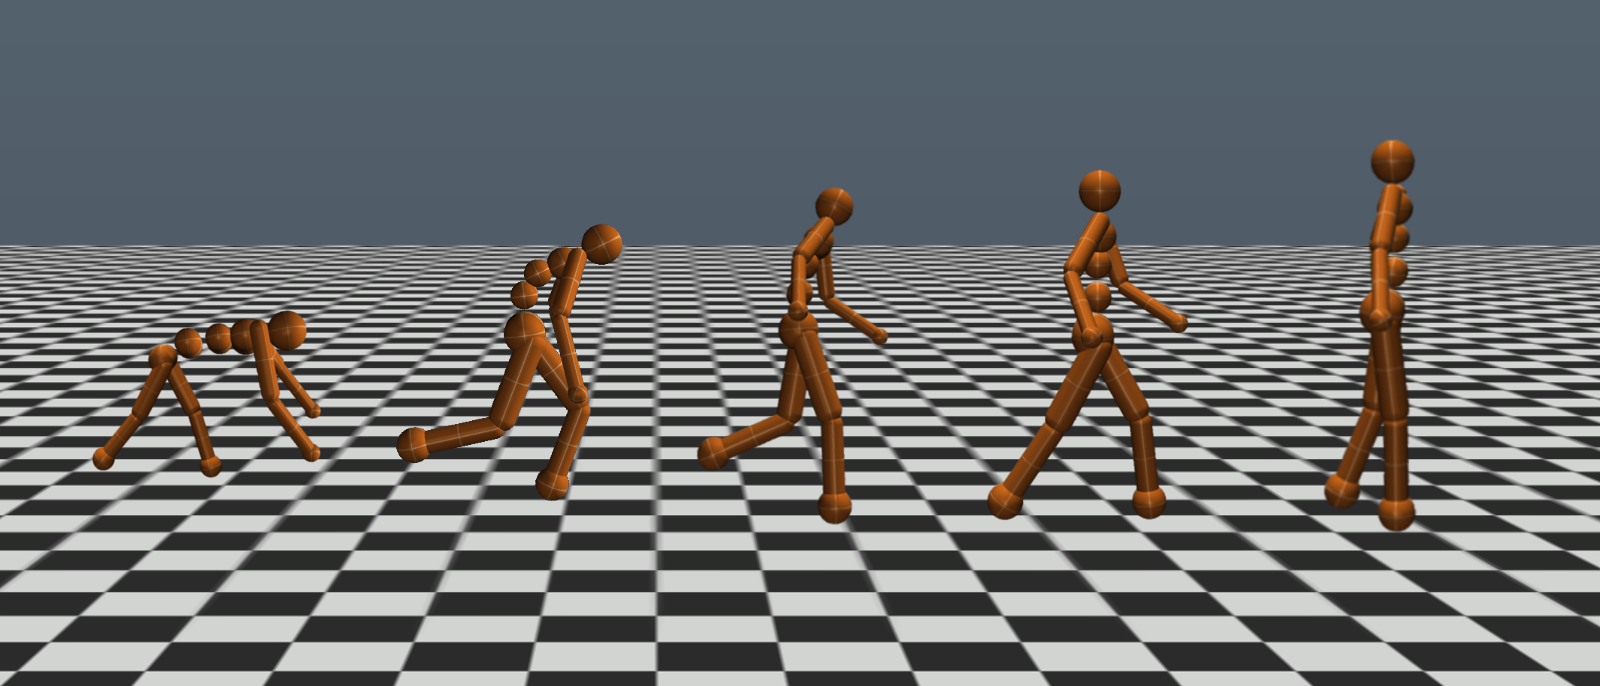
\includegraphics[width=0.9\textwidth]{mujoco_humanoids.png}
    \end{center}
    \label{fig:humanoids_mujoco}
\end{figure}

MuJoCo [[1]] é um \textit{framework} surgido do rápido crescimento do ramo da
robótica e da necessidade dos simuladores utilizados nesta área de acompanhar
o acentuado desenvolvimento --- não apenas em termos de capacidade, como também
tratando-se de complexidade --- deste domínio. O MuJoCo é voltado para o
desenvolvimento de sistemas de controle para robôs, área fundamental da robótica
que visa a automatização de tarefas antes realizadas por humanos ou por outros
sistemas mais simples, porém menos robustos, como é o caso do trabalho
desenvolvido em [[2]], que discursa sobre a modelagem e o refinamento de um
sistema de controle de quadricópteros baseado em otimização Bayesiana.


O MuJoCo é voltado, portanto, para otimização de sistemas de controle, o que
consiste, basicamente, em construir diversas variações de um sistema e
avaliá-las de acordo com um processo que pode ser baseado em inteligência
artificial, com o uso de algoritmos genéticos ou de aprendizado por reforço, por
exemplo. Apesar, entretanto, de ter por objetivo apresentar uma solução para
sistemas de robótica, onde é interessante representar virtualmente sistemas
compostos de diversas partes conectadas de modo relativamente complexo (como é
o caso de braços robóticos) e de possuir uma performance significativamente
melhor do que outras ferramentas da área (no que tange a acurácia da simulação),
o que acarreta em um custo computacional maior, e de possuir certas deficiências
no tocante à simulações que não são normalmente empregadas em problemas de
robótica (MuJoCo é incapaz de reproduzir colisões elásticas, por exemplo),
MuJoCo foi rapidamente
adotado por pesquisadores da área do aprendizado por reforço profundo [[3]]
(abordada brevemente na seção \ref{dqn}), onde algoritmos de aprendizado por
reforço são combinados com redes neurais profundas.


Isto deve-se à facilidade com que modelos podem ser construídos no ambiente
virtual do MuJoCo, o que pode ser feito através de uma descrição de alto nível com
base em um arquivo no formato XML ou de chamadas diretas a uma API que fornece
ao desenolvedor as ferramentas necessárias para a definição de modelos. Dado o
modo simples através do qual objetos podem ser construídos em seu ambiente, é
natural que este \textit{framework} tenha se tornado uma peça importante no
estudo de algoritmos de inteligência artificial quando aplicados em simulações,
mesmo que sua performance em alguns dos cenários apresentados em [[1]] seja
baixa.
Em especial, pode ser citado o caso da DeepMind [[4]], que desenvolveu uma
extensa pesquisa envolvendo as diferentes maneiras com as quais robôs humanóides
(figura \ref{fig:humanoids_mujoco}) aprendem a se locomover de acordo com a
maneira através da qual a noção de recompensa é representada.


Devido, entretanto, ao seu alto grau de especificidade (o MuJoCo foi feito
especialmente para atender às demandas do ramo da robótica, onde motores de
simulações físicas voltados para jogos não são acurados o suficiente --- há
casos, por exemplo, onde a simulação aprende a explorar falhas do motor de
física, que não condizem com a realidade [[5]]), há casos onde o
\textit{framework} pode ser considerado complexo demais, não só pela sua
extensa documentação sobre as funções da sua API para criação de corpos e
conectores, como também pelo seu conjunto de algoritmos de cálculos físicos, que
fornecem uma lista bastante abrangente de informações sobre os corpos
representados na simulação. Além do mais, há a questão do custo: o MuJoCo não
é um \textit{software} livre, sendo oferecido de graça apenas para integrantes
da comunidade científica. Para os demais, sua licença é oferecida a preços que
variam de quinhentos a dois mil dólares.

\section{Simuladores com interface para Aprendizado de máquina}
\blindtext
\subsection{Unity-ML}
\subsection{Gym}
\subsubsection{ALE}
\subsubsection{VizDoom}
\subsubsection{Arquitetura do Gym}
\subsubsection{DART}
Voltado, assim como o \textit{MuJoCo}, para simulações envolvendo robótica,
a ferramenta chamada \textit{DART} (de \textit{Dynamie Animation and Robotics
Toolkit}) foi desenvolvida em 2012. Nos testes apresentados em [[1]], apresentou
um comportamento regular, exceto no teste de fricção, onde os objetos simulados
não se comportaram da maneira esperada.

Em todos os cenários de teste, \textit{DART} apresentou o pior desempenho em
todos eles, apresentando imprecisões grotescas no cenário que envolve fricção.
Apesar de não possuir um desempenho excepcional, entretanto, \textit{DART} foi
adotada como
um dos motores de física que formam a base do simulador \textit{Gazebo}, voltado
especialmente para a robótica. O simulador é capaz de importar arquivos que,
utilizando uma sintaxe própria, definem robôs e criá-los no ambiente simulado de
uma maneira relativamente simples. Mais sobre o \textit{Gazebo} na seção
\ref{gazebo}.



\section{Simuladores de Aprendizado por Reforço}

% [1] http://www2.islab.ntua.gr/attachments/article/67/Super%20Mario%20Evolution.pdf
% [2] https://arxiv.org/pdf/1506.08941.pdf


Conforme desenvolvido anteriormente, algoritmos de aprendizado por reforço
possuem uma vasta série de aplicações: seja jogos de tabuleiro, máquinas que
aprendem por si mesmas a jogar diversos jogos de computador ou sistemas de
controle de veículos autônomos, algoritmos de AR são recomendados em quaisquer
situações onde ações devem ser tomadas de maneira sequencial por um agente
inserido dentro de um ambiente, com o qual ele interage através da sua sucessão
de decisões tomadas. Problemas diferentes, portanto, requerem diferentes meios
de simulação: um agente que joga xadrez, por exemplo, pode ser treinado
usando-se de um simulador que representa o tabuleiro através de uma matriz, onde
cada célula guarda a informação da peça ali presente, caso haja alguma. Um outro
simulador, publicado em 2009 [[1]], que treina um agente para jogar o jogo
\textit{Super Mario World}, baseia-se em uma adaptação do modo com que os
diferentes níveis do jogo eram representados no \textit{Super Nintendo}, seu
\textit{console} de origem.


Visto que problemas diferentes requerem maneiras distintas de representar-se o
ambiente no qual os agentes estão inseridos e com os quais eles interagem, é
necessário definir a estrutura básica, comum a qualquer simulação, de um
problema de aprendizado por reforço. É natural que, ao pensarmos na palavra
"simulador", nos venha à mente algum tipo de ferramenta essencialmente visual,
como o simulador utilizado em autoescolas da figura
\ref{fig:simuladorautoescola}. Entretanto, quando se trata de aprendizado por
reforço, nem sempre há utilidade em construir visualmente o ambiente e o agente
nele inserido: como no caso do tabuleiro de xadrez, representá-lo através de
figuras visuais é desnecessário.


Tratanto-se de aprendizado por reforço, portanto, o componente visual nem sempre
faz parte da essência do simulador. Por vezes, é util que este seja ignorado
para que os recursos que seriam consumidos por algoritmos de computação gráfica
sejam transferidos às tarefas ligadas ao treinamento do agente e, em alguns
casos, é até mesmo impossível representar o problema de uma forma essencialmente
visual [[2]]. Sendo assim, resta definir qual é o elemento fundamental de um
simulador, quando dentro de um contexto de treinamento de agentes através de
algoritmos de aprendizado por reforço.

\begin{figure}
    \caption{Ciclo de aprendizado do agente via interação com o ambiente}
    \begin{center}
      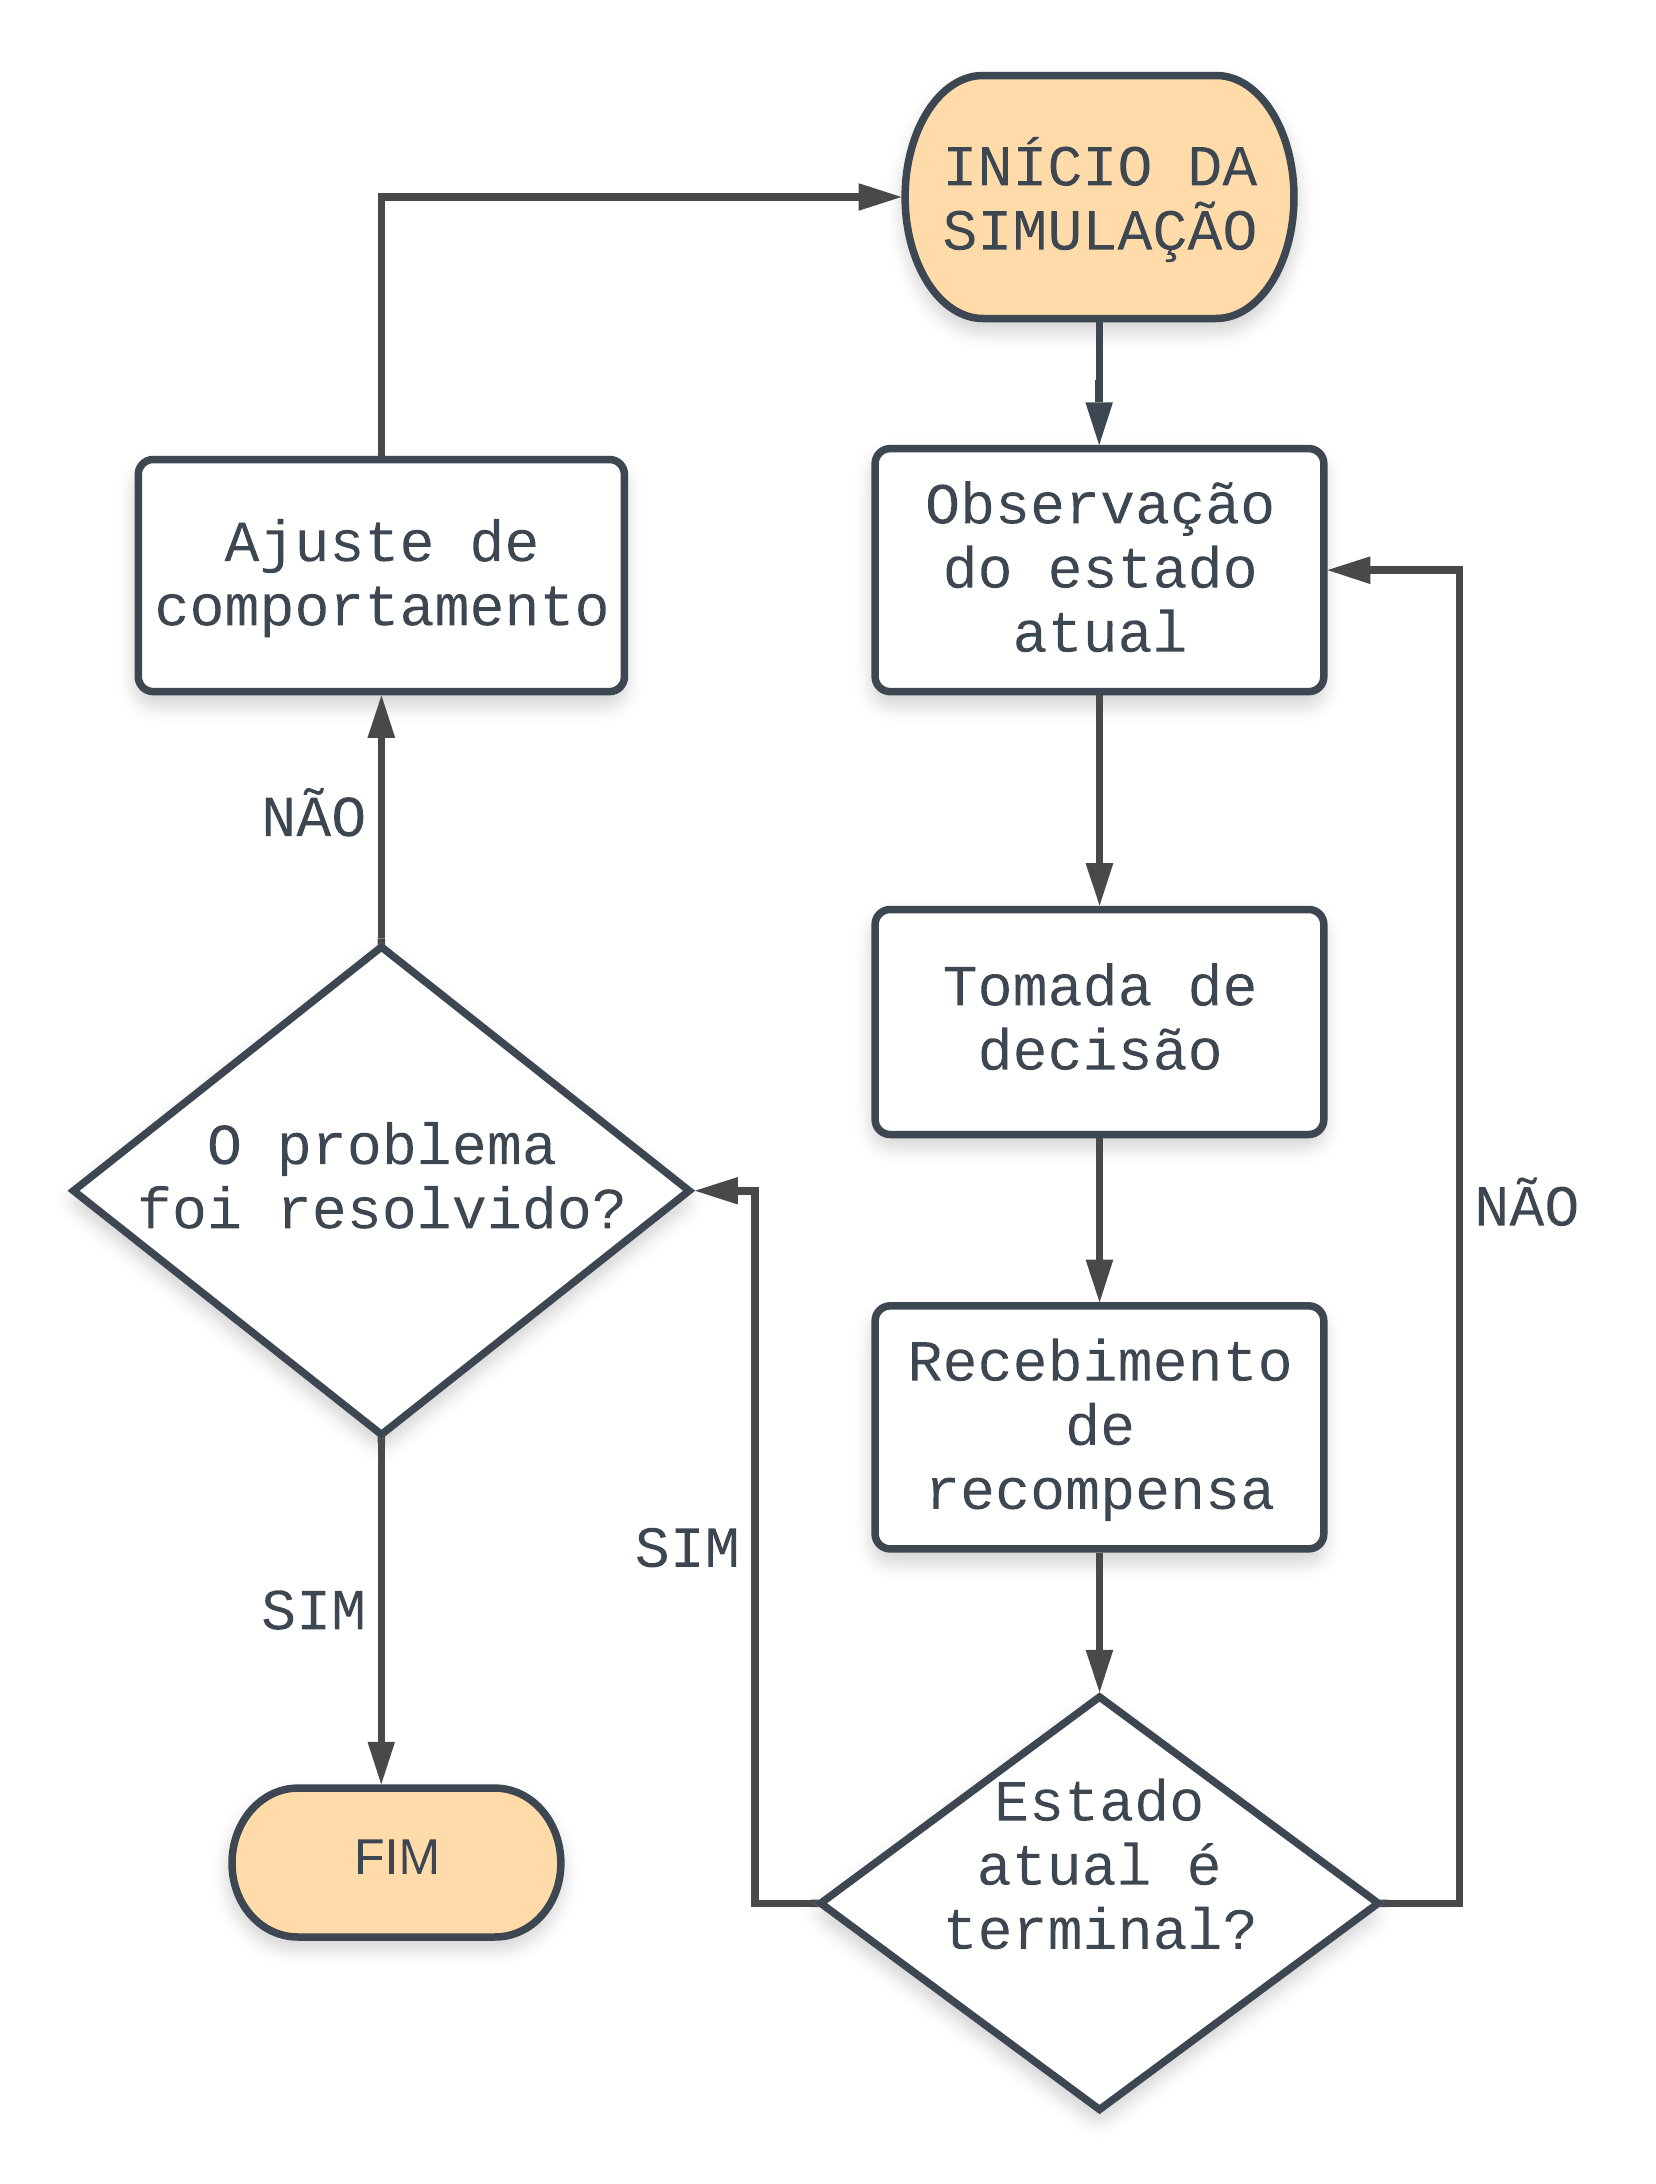
\includegraphics[width=0.65\textwidth]{fluxo_ar.png}
    \end{center}
    \label{fig:fluxo_ar_old}
\end{figure}


E qual a peça principal de um sistema modelado por um Processo de Decisão de
Markov? Bom, é natural que seja, exatamente, o MDP e seus subcomponentes:
as informações a respeito do ambiente, as ações possíveis que podem ser tomadas
em um estado, a noção de recompensa pela ação tomada e a transição entre estados
derivada de uma ação. O componente fundamental de uma simulação de aprendizado
por reforço é, portanto, o conjunto dos elementos envolvidos em um processo de
decisão markoviano e as relações que os diferentes elementos travam entre si,
como as transições entre estados decorrentes das ações tomadas pelo agente e as
recompensas recebidas pelas ações tomadas. Conclui-se, portanto, que componentes
visuais são secundários, podendo ou não estar presentes na simulação: mais
importante que quaisquer ferramentas gráficas é o ciclo de aprendizado de um
agente de aprendizado por reforço, descrito na figura \ref{fig:fluxo_ar}.


Um simulador de aprendizado por reforço é, portanto, uma ferramenta que combina
o ciclo descrito na figura \ref{fig:fluxo_ar} com alguma outra ferramenta que
permita que sejam representados os componentes de um Processo de Decisão de
Markov: o ambiente, o agente nele inserido, as ações possíveis em cada época de
decisão e a noção de recompensa, sem que, necessariamente, haja uma
representação visual destes. A ferramenta \textit{VizDoom} [[5]], por exemplo,
permite que algoritmos de aprendizado por reforço sejam aplicados ao jogo de
tiro em terceira pessoa \textit{Doom}, tendo se tornado uma ferramenta
importante de avaliação de algoritmos de AR. Há evidentemente, uma construção
visual dos objetos (i.e. o jogador, o mapa e os inimigos), mas também há, no
cerne do \textit{software}, estruturas de dados internas que representam o
estado atual do jogo e das quais o agente extrai as informações necessárias para
suas tomadas de decisão. As seções seguintes deste capítulo tratarão de
ferramentas normalmente utilizadas para a construção de simuladores de
aprendizado por reforço, explicitando seus destaques positivos e suas
deficiências, bem como suas aplicações mais comuns.


\section{Construindo um simulador de aprendizado por reforço}


\begin{figure}[h]
    \caption{O problema conhecido como \textit{Frozen Lake}}
    \begin{center}
      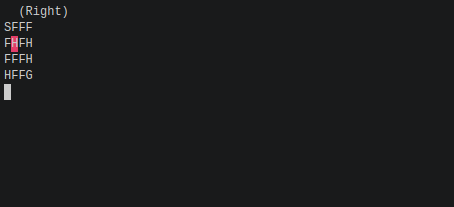
\includegraphics[width=0.5\textwidth]{frozen_lake.png}
    \end{center}
    \label{fig:frozen_lake}
\end{figure}


Para construir um simulador de AR, conforme desenvolvido anteriormente, não é
estritamente necessária a presença de um componente visual. É preciso,
entretanto, que a arquitetura do simulador contenha os componentes de um MDP e
que as relações entre eles se deem corretamente, em um ciclo próximo do que é
descrito na imagem \ref{fig:fluxo_ar}. Estas são as premissas básicas para a
construção de um simulador de aprendizado por reforço e qualquer construção que
vá além desta definição irá depender da natureza do problema a ser resolvido, o
que pode exigir o uso de ferramentas mais complexas, como motores de física, que
buscam aproximar o comportamento de corpos no espaço tridimensional da maneira
como ocorre no mundo real, ou o emprego de ferramentas mais simples. Um exemplo
de problema bastante trivial, que pode ser construído em um simulador sem que
seja necessário nada além de estruturas básicas de dados e representação visual
em modo texto é um problema chamado \textit{Frozen Lake}: o problema descreve
um homem que precisa andar por sobre um lago congelad, saindo de um ponto de
partida e com destino a um ponto de chegada, previamente conhecido. O lago
apresenta lugares,
porém, onde a camada de gelo é fina demais para suportar o peso do homem, que
cairá na água caso tente passar por eles. Cabe ao agente, portanto, aprender a
controlar o homem por sobre o lago, sabendo de onde ele sai, para onde ele deve
se dirigir e quais pontos no lago não podem ser perpassados. Para representar o
lago, apenas uma matriz de caracteres é necessária, com símbolos distintos para
representar o ponto de partida, o ponto de chegada, os pontos onde é seguro
atravessar e os pontos onde o gelo é fino demais. Uma matriz de tamanho
arbitrário, descrita na tela de um \textit{console}, portanto, é capaz de
fornecer uma representação completa do problema, como é o caso na imagem
\ref{fig:frozen_lake}.


Cabe esclarecer, entretanto, que o caso do problema \textit{Frozen Lake} é
bastante especial, uma vez que o problema é comumente utilizado apenas para fins
didáticos, como exemplo de uso de técnicas simples de resolução de Processos de
Markov como as exibidas no capítulo \ref{basic_concepts}. É natural que o uso
de simuladores mais complexos, que tenham a capacidade de representar estados
definidos por um volume maior de informações, sejam empregados quando o problema
em questão envolve mais elementos do que uma simples matriz que representa um
lago congelado.


É este o caso no ramo da robótica, por exemplo. Qualquer tarefa que necessite
ser executada repetidamente e com certo grau de precisão é uma boa candidata
para a automatização através do emprego de robôs: linhas de montagem de
empresas automotivas, por exemplo, já são dominadas por robôs há varios anos.
Outras tarefas, mais complexas do que as executadas pelos robôs da manufatura,
mas ainda assim consideradas maçantes e repetitivas por humanos --- como
dirigir, por exemplo ---, também são fortes candidatas à automação, tendo, nos
últimos tempos, sido alvo de pesquisas de ponta envolvendo inteligência
artificial, com a popularização de técnicas de aprendizado de máquina e visão
computacional. É aí que entra o uso de simuladores: durante as fases iniciais
de desenvolvimento de um robô, uma versão virtual deste pode ser construída,
como na figura \ref{fig:mujoco_robot}, em um ambiente fundamentado em motores
de física que simulam as leis do mundo real. No ambiente controlado de um
simulador, o treinamento do agente pode ser feito de forma acelerada, fazendo
com que as primeiras versões reais do robô já apresentem uma versão incial do
comportamento que quer-se ensinar a ele.

\begin{figure}[h]
    \caption{Um robô real e sua versão modelada em um simulador.}
    \begin{center}
      \frame{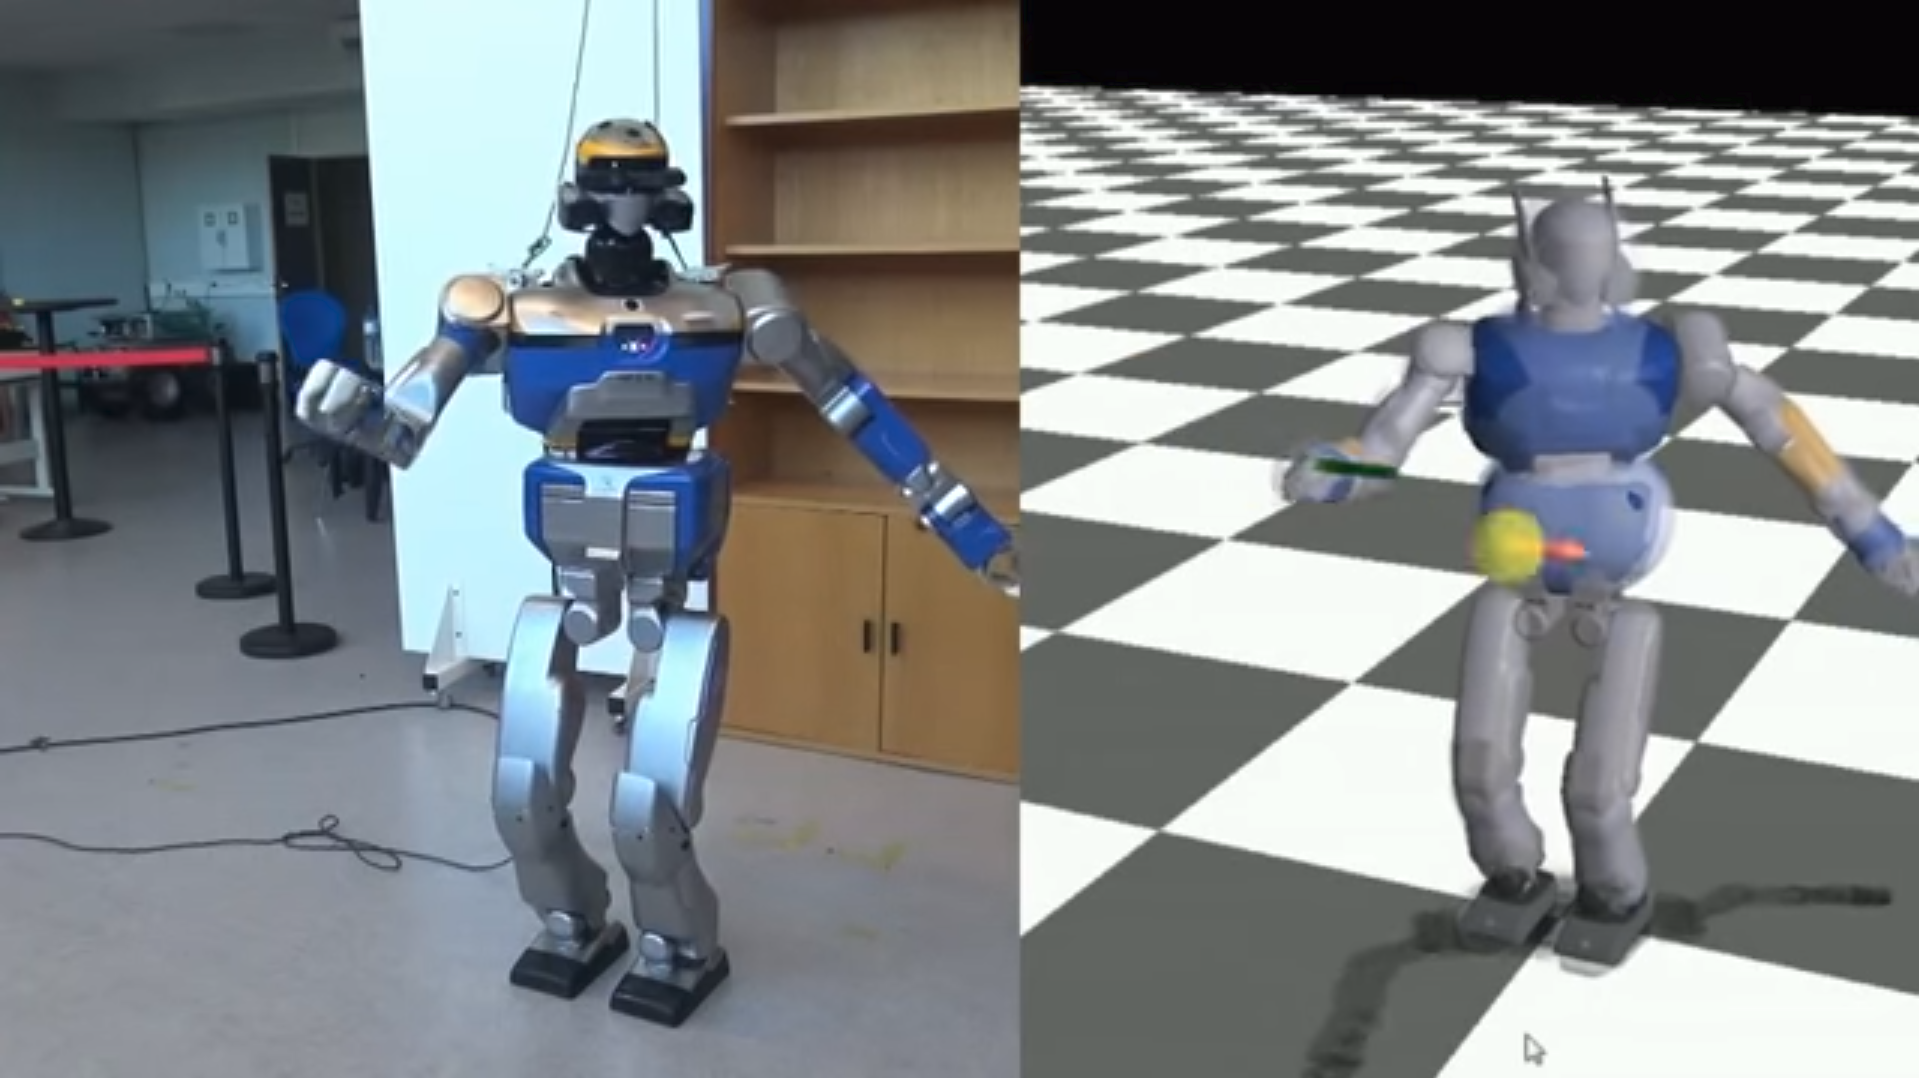
\includegraphics[width=0.9\textwidth]{mujocosimulator.png}}
    \end{center}
    \label{fig:mujoco_robot}
\end{figure}

\subsection{Motores de Física}
% [[1]] https://leggedrobotics.github.io/SimBenchmark/
% [[2]] D. Kaufman et al., “Staggered projections for
%       frictional contact in multibody systems,” 2008.

Robôs interagem com o mundo ao seu redor através do contato físico com o
ambiente que os cerca. É primordial, portanto, para o treinamento de um robô,
que existam ferramentas capazes
de reconstruir, em um ambiente virtual e controlado, não apenas seu aspecto
físico (i.e. as diferentes partes que o constituem) e do ambiente no qual ele
está inserido, mas também de simular, tão próximo quanto possível --- ou
desejado --- da realidade, as forças envolvidas na interação do robô com o
ambiente. Para isso, um simulador deve definir os corpos no espaço e calcular
as forças resultantes do contato entre eles, o que é um problema NP-Difícil [[2]]
e, portanto, computacionalmente custoso.
É possível, porém, tornar o problema tratável através da sua aproximação
utilizando-se de métodos de programação linear. Diferentes métodos possuem
diferentes abordagens: alguns, mais precisos, requerem mais recursos
computacionais, enquanto outros sacrificam parte da precisão de seus resultados
em troca de soluções mais rápidas. Felizmente, nenhum destes métodos precisa ser
implementado do zero, uma vez que existem diversos motores de física que
resolvem este tipo de problema. Alguns, normalmente utilizados em jogos
eletrônicos, utilizam métodos mais simples para o cálculo das forças
físicas resultantes do contato, uma vez que, pelo menos nos jogos, a precisão
dos contatos simulados é menos importante do que o número de quadros processados
por segundo. Outros, por sua vez, utilizados em aplicações industriais --- onde
normalmente o objetivo são simulações com o máximo de precisão ---, utilizam
técnicas que consomem mais processamento, mas que entregam um resultado mais
fidedigno.


Em [[1]], uma análise de diferentes motores de física é realizada, com o
objetivo de comparar a performance deles em diferentes situações. No estudo,
uma espécie de avaliação qualitativa dos \textit{softwares} é conduzida,
analisando-se duas características intrínsecas às simulações: velocidade e
acurácia.


É natural que queira-se um simulador que apresente simulações altamente
fidedignas no menor tempo possível. O que acontece normalmente, entretanto, é
uma espécie de \textit{trade-off} entre estas duas qualidades: quando simulações
precisam ser fiéis, o que consome mais recursos computacionais, os resultados
demoram para ser entregues, o que faz com que as simulações sejam mais
vagarosas. Por outro lado, quando é desejável que os resultados sejam entregues
rapidamente, simulações mais simples são conduzidas, abrindo-se mão de parte da
qalidade dos resultados. Alguns dos motores apresentados fornecem simulações
robustas, porém mais lentas; outros, por sua vez, por serem voltados à
aplicações visuais, realizam as simulações mais rapidamente, mas com perda de
precisão.


Dos cinco motores analisados, um deles ainda está em fase de desenvolvimento e,
portanto, não foi incluído neste trabalho. Todos foram submetidos aos seguintes
cenários, que cobrem interações entre objetos formados por um único corpo e por
robôs formados por múltiplos corpos interconectados:

\begin{itemize}
  \item \textit{Rolling test}: teste de modelos de fricção;
  \item \textit{Bouncing test}: teste de colisão elástica envolvendo um corpo;
  \item \textit{666 balls test}: teste de colisão sólida envolvendo múltiplos
  corpos;
  \item \textit{Elastic 666 balls test}: teste de colisão elástica envolvendo
  múltiplos corpos;
  \item \textit{ANYmal PD control test}: teste de velocidade de um robô
  quadrúpede;
  \item \textit{ANYmal momentum test}: teste de impulso de um robô articulado;
  \item \textit{ANYmal energy test}: teste de energia de um robô articulado;
\end{itemize}


\subsubsection{DART}
Voltado, assim como o \textit{MuJoCo}, para simulações envolvendo robótica,
a ferramenta chamada \textit{DART} (de \textit{Dynamie Animation and Robotics
Toolkit}) foi desenvolvida em 2012. Nos testes apresentados em [[1]], apresentou
um comportamento regular, exceto no teste de fricção, onde os objetos simulados
não se comportaram da maneira esperada.

Em todos os cenários de teste, \textit{DART} apresentou o pior desempenho em
todos eles, apresentando imprecisões grotescas no cenário que envolve fricção.
Apesar de não possuir um desempenho excepcional, entretanto, \textit{DART} foi
adotada como
um dos motores de física que formam a base do simulador \textit{Gazebo}, voltado
especialmente para a robótica. O simulador é capaz de importar arquivos que,
utilizando uma sintaxe própria, definem robôs e criá-los no ambiente simulado de
uma maneira relativamente simples. Mais sobre o \textit{Gazebo} na seção
\ref{gazebo}.

\subsubsection{MuJoCo}
% [1] https://ieeexplore.ieee.org/abstract/document/6386109
% [2] controller optimization => https://arxiv.org/abs/1509.01066
% [3] http://proceedings.mlr.press/v48/mniha16.pdf
% [4] https://arxiv.org/pdf/1707.02286.pdf
% [5] http://people.reed.edu/~jimfix/math385/lec01.1/Animation/p15-sims-evolving.pdf

\label{mujoco}

\begin{figure}[h]
    \caption{Modelagem de robôs humanoides no ambiente do MuJoCo}
    \begin{center}
      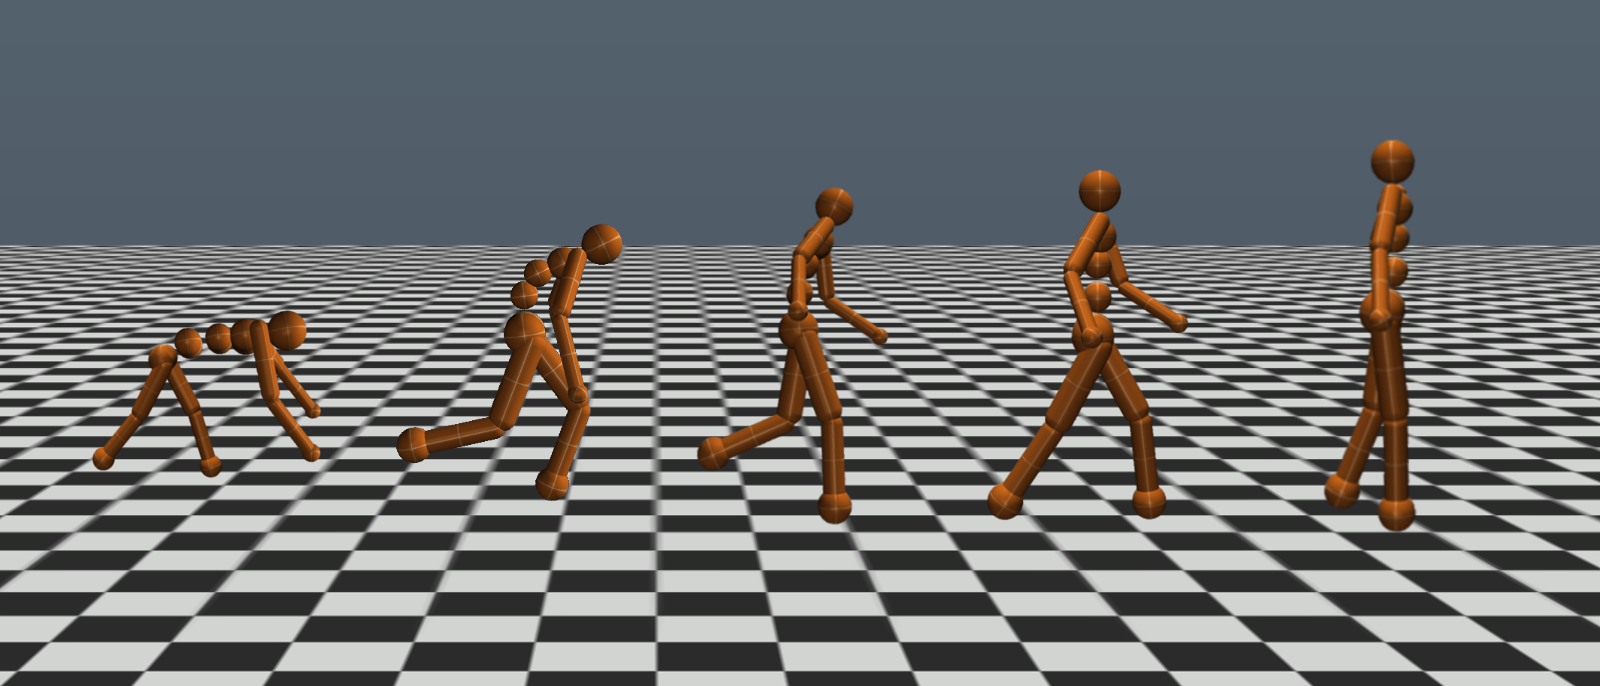
\includegraphics[width=0.9\textwidth]{mujoco_humanoids.png}
    \end{center}
    \label{fig:humanoids_mujoco}
\end{figure}

MuJoCo [[1]] é um \textit{framework} surgido do rápido crescimento do ramo da
robótica e da necessidade dos simuladores utilizados nesta área de acompanhar
o acentuado desenvolvimento --- não apenas em termos de capacidade, como também
tratando-se de complexidade --- deste domínio. O MuJoCo é voltado para o
desenvolvimento de sistemas de controle para robôs, área fundamental da robótica
que visa a automatização de tarefas antes realizadas por humanos ou por outros
sistemas mais simples, porém menos robustos, como é o caso do trabalho
desenvolvido em [[2]], que discursa sobre a modelagem e o refinamento de um
sistema de controle de quadricópteros baseado em otimização Bayesiana.


O MuJoCo é voltado, portanto, para otimização de sistemas de controle, o que
consiste, basicamente, em construir diversas variações de um sistema e
avaliá-las de acordo com um processo que pode ser baseado em inteligência
artificial, com o uso de algoritmos genéticos ou de aprendizado por reforço, por
exemplo. Apesar, entretanto, de ter por objetivo apresentar uma solução para
sistemas de robótica, onde é interessante representar virtualmente sistemas
compostos de diversas partes conectadas de modo relativamente complexo (como é
o caso de braços robóticos) e de possuir uma performance significativamente
melhor do que outras ferramentas da área (no que tange a acurácia da simulação),
o que acarreta em um custo computacional maior, e de possuir certas deficiências
no tocante à simulações que não são normalmente empregadas em problemas de
robótica (MuJoCo é incapaz de reproduzir colisões elásticas, por exemplo),
MuJoCo foi rapidamente
adotado por pesquisadores da área do aprendizado por reforço profundo [[3]]
(abordada brevemente na seção \ref{dqn}), onde algoritmos de aprendizado por
reforço são combinados com redes neurais profundas.


Isto deve-se à facilidade com que modelos podem ser construídos no ambiente
virtual do MuJoCo, o que pode ser feito através de uma descrição de alto nível com
base em um arquivo no formato XML ou de chamadas diretas a uma API que fornece
ao desenolvedor as ferramentas necessárias para a definição de modelos. Dado o
modo simples através do qual objetos podem ser construídos em seu ambiente, é
natural que este \textit{framework} tenha se tornado uma peça importante no
estudo de algoritmos de inteligência artificial quando aplicados em simulações,
mesmo que sua performance em alguns dos cenários apresentados em [[1]] seja
baixa.
Em especial, pode ser citado o caso da DeepMind [[4]], que desenvolveu uma
extensa pesquisa envolvendo as diferentes maneiras com as quais robôs humanóides
(figura \ref{fig:humanoids_mujoco}) aprendem a se locomover de acordo com a
maneira através da qual a noção de recompensa é representada.


Devido, entretanto, ao seu alto grau de especificidade (o MuJoCo foi feito
especialmente para atender às demandas do ramo da robótica, onde motores de
simulações físicas voltados para jogos não são acurados o suficiente --- há
casos, por exemplo, onde a simulação aprende a explorar falhas do motor de
física, que não condizem com a realidade [[5]]), há casos onde o
\textit{framework} pode ser considerado complexo demais, não só pela sua
extensa documentação sobre as funções da sua API para criação de corpos e
conectores, como também pelo seu conjunto de algoritmos de cálculos físicos, que
fornecem uma lista bastante abrangente de informações sobre os corpos
representados na simulação. Além do mais, há a questão do custo: o MuJoCo não
é um \textit{software} livre, sendo oferecido de graça apenas para integrantes
da comunidade científica. Para os demais, sua licença é oferecida a preços que
variam de quinhentos a dois mil dólares.


\section{Simuladores existentes}
Apesar de executarem as tarefas para as quais foram propostos com bastante
eficiência, os motores de física, sozinhos, não possuem a capacidade de
construir uma simulação voltada para aprendizado por reforço, pois é preciso
mais do que técnicas de resolução de forças vetoriais para dar inteligência a um
agente. Um simulador de aprendizado por reforço precisa não só de um ambiente
virtual (tal como os oferecidos pelos motores de física, mas sem que os
ambientes possíveis estejam restritos aos fornecidos por eles), mas também de
estruturas que representem as informações que representam os elementos
envolvidos no ciclo de aprendizado de um agente de AR, como descrito na figura
\ref{fig:fluxo_ar}.


Felizmente, dependendo da natureza do agente e do problema que ele tenta
resolver, não é necessário desenvolver um simulador de aprendizado por reforço
completamente do zero. Há diversos \textit{softwares} disponíveis no mercado que
fornecem as ferramentas necessárias para treinar um agente sem que seja
necessário preocupar-se com os elementos básicos envolvidos no treinamento,
ficando a encargo do desenvolvedor somente a formulação do problema e do método
de aprendizado.


Há uma série de problemas, de naturezas muito distintas, que técnicas de
aprendizado por reforço se propõem a resolver. É bastante diverso, justamente
por isso, o universo de simuladores de agentes de AR. O desenvolvimento de um
trabalho na área envolve, portanto, uma análise cuidadosa das ferramentas que
serão utilizadas para a construção da simulação do problema: um
\textit{software} de propósito mais geral, por exemplo, pode ser utilizado sem
problema algum para formular e resolver um problema do campo da robótica. Um
outro \textit{software}, voltado apenas para formulação de problemas desta área,
entretanto, pode ser uma escolha melhor neste caso, uma vez que seu objetivo é
justamente simplificar tarefas deste tipo.


Três \textit{softwares} para a formulação de problemas e treinamento de agentes
de AR são apresentados a seguir. Um deles é voltado para o campo da robótica,
outro para a construção de cenários típicos de jogos eletrônicos ou de
tabuleiro, enquanto o terceiro, sendo um \textit{framework} de propósito mais
geral, apresenta uma coleção mais variada de ferramentas e de algoritmos
pré-estabelecidos de treinamento, com o intuito de servir de base comparativa.

\subsection{Gazebo}
% [[1]] http://citeseerx.ist.psu.edu/viewdoc/download?doi=10.1.1.304.8999&rep=rep1&type=pdf
% [[2]] https://www.willowgarage.com/sites/default/files/icraoss09-ROS.pdf

\textit{Gazebo} [[1]] é uma ferramenta voltada para a simulação de cenários envolvendo
problemas de robótica. Dotada de uma interface gráfica que auxilia na criação
de ambientes tridimensionais e dos robôs nele inseridos, \textit{Gazebo}
facilita enormemente o trabalho de pesquisadores e desenvolvedores da área de
robótica, uma vez que fornece meios de definir robôs e ambientes através de uma
linguagem própria de marcação, o que não só simplifica o trabalho de
desenvolvimento, mas também estimula o compartilhamento de diferentes modelos
entre os membros da comunidade.


\textit{Gazebo} é compatível com um sistema chamado \textit{ROS} [[2]] --- de
\textit{Robot Operating System}, ou Sistema Operacional de Robôs, em tradução
livre ---, que agrupa uma série de bibliotecas, ferramentas e convenções que
visam não apenas simplificar a tarefa de desenvolver um robô, mas também de
estabelecer normas e padrões a fim de que seja facilitada e estimulada a
colaboração entre pesquisadores de diversas instituições. Assim como no
\textit{software} fornecido pelo \textit{Gazebo}, \textit{ROS} também fornece
uma linguagem própria de marcação pela qual é possível definir robôs e o espaço
no qual eles estão inseridos. O formato também é compreendido pelo
\textit{Gazebo}, simplificando o intercâmbio de informações entre os dois
sistemas.


Conforme descrito em [[1]], \textit{Gazebo} oferece um meio de integrar
descrições textuais de alto nível de robôs e de ambientes com diferentes motores
de física, incluindo \textit{Bullet Physics}, \textit{DART} e \textit{ODE}, com
\textit{ODE} sendo o padrão, podendo ser facilmente substituído. Esta é a grande
vantagem oferecida por \textit{Gazebo} àqueles que decidem adotar seu
\textit{software}: é oferecido aos desenvolvedores e pesquisadores um ambiente
rico e agnóstico quanto às ferramentas utilizadas, uma vez que vários sistemas
amplamente usados são compatíveis com \textit{Gazebo}. Além disso, o
\textit{software} não tem custo e seu código é aberto, o que sifnifica que ele
pode ser alterado e qualquer pessoa pode contribuir com mudanças e adições nele.
Isto possibilitou que florescesse uma comunidade bastante ativa de pessoas
dispostas a contribuir com o projeto, desenvolvendo modelos de robôs e ambientes
com o objetivo de compartilhá-los. Todo o material já produzido pela comunidade,
aliado às ferramentas que o \textit{software} disponibiliza para a rápida
criação de modelos e ambientes, é o que faz o \textit{Gazebo} ser o que é. Seu
uso é tão simples que ele é utilizado até por alunos de graduação, inclusive
na UFRGS.


\subsection{Unity ML-Agents Toolkit}

\begin{figure}[h]
    \caption{Imagem do jogo \textit{Puppo}}
    \begin{center}
      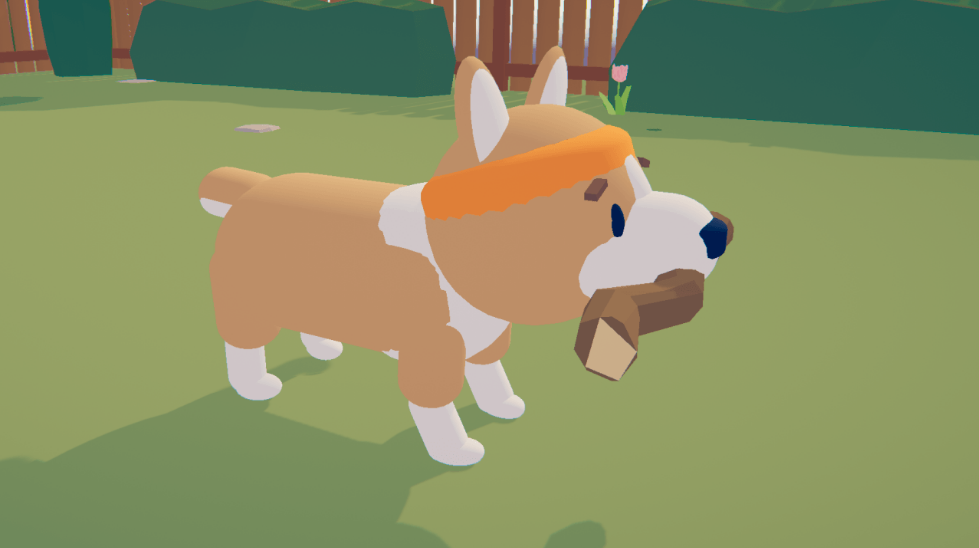
\includegraphics[width=0.9\textwidth]{puppo.png}
    \end{center}
    \label{fig:puppo}
\end{figure}

% [[1]] https://arxiv.org/pdf/1809.02627.pdf
% [[2]] https://blogs.unity3d.com/2018/10/02/puppo-the-corgi-cuteness-overload-with-the-unity-ml-agents-toolkit/

A biblioteca chamada de \textit{Unity ML-Agents} [[1]] nada mais é do que uma
extensão do \textit{software} chamado \textit{Unity}, programa que possui um
motor próprio de física tridimensional e que é voltado para o desenvolvimento de
jogos eletrônicos. A extensão, proposta em 2018, fornece uma série de
ferramentas para aqueles que querem rodar simulações de problemas de
inteligência artificial dentro do ambiente da \textit{Unity}. Apesar de ter sido
desenvolvida como uma plataforma de propósitos gerais, por causa da natureza
do sistema sobre o qual ela foi incorporada, muitas das aplicações envolvem
simulações de jogos, onde agentes aprendem a competir entre si.


Um dos princípios básicos que guiou a equipe responsável pelo desenvolvimento
da \textit{Unity ML-Agents Toolkit} foi possibilitar que desenvolvedores e
estúdios de jogos eletrônicos incorporassem técnicas de inteligência artificial
em suas obras utilizando técnicas atuais, como as redes neurais descritas na
seção \ref{dqn}. Como forma de promover a plataforma e demonstrar suas capacidades,
pesquisadores da Unity exibiram, em um evento em meados de 2018, o jogo
\textit{Puppo} [[2]], onde um cachorro busca um graveto atirado pelo jogador
através de toques na tela (figura \ref{fig:puppo}). O agente responsável pelos
movimentos do cachorro, neste caso, foi treinado inteiramente utilizando-se de
algoritmos de Aprendizagem por Reforço Profunda.


Dada a natureza do programa que serve de base para o simulador e o enfoque dado
às ferramentas fornecidas por ele, fica claro que o interesse dos
desenvolvedores é estimular o treinamento e uso de agentes nos jogos
desenvolvidos na plataforma \textit{Unity}. Problemas de robótica, por exemplo,
são modelados e resolvidos de uma maneira muito mais simples e prática através
de outras ferramentas, como a \textit{Gazebo}. Fica claro, portanto, o foco dado
ao \textit{Unity ML-Agents Toolkit}: facilitar a vida daqueles que pretendem
utilizar inteligência artificial no universo de jogos eletrônicos.


\subsection{Baselines}
% [1] https://openai.com/blog/openai-baselines-dqn/
Desenvolvido pela OpenAI, uma organização sem fins lucrativos que realiza
estudos na área de inteligência artificial, a ferramenta \textit{Baselines}
surgiu como uma tentativa de criar-se uma espécie de padronização para a
avaliação de algoritmos a serem propostos pela comunidade de pesquisadores e
desenvolvedores da área de aprendizado por reforço. No artigo que apresenta a
ferramenta [[1]], os responsáveis pela ferramenta deixam claro que seu objetivo
é permitir que, no momento que um algoritmo é proposto e precisa ser avaliado,
haja uma espécie de "parâmetro comum", que seja amplamente conhecido e que sirva
de base para comparações. O \textit{software} oferece uma vasta coleção de
simuladores, que vão desde representações de problemas conhecidos da literatura
até simulações de plataformas antigas de jogos eletrônicos.


\textit{Baselines} possui uma coleção bastante diversa de cenários e de
algoritmos, o que é um mais um indício do foco dado ao projeto pelos seus
desenvolvedores: o objetivo maior do \textit{Baselines} não é trazer comodidade
a quem realiza pesquisas em uma determinada área da inteligência artificial,
como o \textit{Gazebo} se propõe a oferecer auxílio àqueles que desenvolvem
trabalhos no ramo da robótica. Em vez disso, \textit{Baselines} se compromete
a fornecer uma coleção padrão de problemas e implementações de algoritmos
para servir de base a estudos futuros, como uma espécie de base de comparação.
Conforme o artigo que apresenta a ferramenta, inteligência artificial é uma
ciência empírica, na qual a praticidade em conduzir experimentos está
diretamente relacionada ao progresso no campo. \textit{Baselines} fornece uma
série de implementações de algoritmos já estudados e ferramentas para medir
suas performances em uma coleção variada de problemas para poupar pesquisadores
do trabalho de implementá-los novamente.


Um detalhe deve ser observado, entretanto: \textit{Baselines} não permite que
quem estiver desenvolvendo algoritmos novos teste-os em seus ambientes
simulados, possibilitanto apenas que algoritmos presentes em sua coleção sejam
empregados nos cenários. É possível medir sua performance e gerar gráficos que
representem, por exemplo, o aumento na recompensa recebida pelo agente ao longo
do treinamento. \textit{Baselines} falha, porém, ao impossibilitar que novos
métodos de treinamento de agentes sejam empregados em seus cenários, o que
poderia possibilitar, por exemplo, que as curvas de aprendizado de um agente
treinado com dois algoritmos diferentes, um externo e um interno de sua
biblioteca, fossem meticulosamente comparadas.


É da necessidade de ter-se ferramentas que forneçam cenários de teste para
vários algoritmos diferentes, para que estes possam ter suas performances
comparadas quando submetidas às mesmas condições, que surgiram as ferramentas de
\textit{benchmark}. As três mais conhecidas são apresentadas e analisadas a
seguir.


\section{Ferramentas de \textit{Benchmark}}
\label{benchmark}

Em se tratando de aprendizado por reforço, ferramentas de \textit{benchmark}
servem para fornecer uma base padronizada de avaliação de algoritmos, o que
significa que elas nada mais são do que um meio padronizado de comparar a
performance de diferentes técnicas de aprendizado quando submetidas a um mesmo
problema de aprendizado por reforço. Tais coleções permitem, por exemplo, que
um algoritmo que está sendo desenvolvido seja comparado, em uma série de
problemas, com diferentes outros algoritmos consagrados, a fim de que seja
estudado o seu comportamento em diferentes situações.


Dado que problemas de aprendizado por reforço lidam com cenários onde um agente
deve tomar uma série de ações em sequência, é natural que tenha surgido no ramo
uma série de pesquisas e algoritmos que tentam ensinar agentes dotados de
inteligência artificial a jogar diversos jogos eletrônicos. Duas coleções de
cenários do tipo, que reproduzem jogos famosos de plataformas antigas (ou seja,
mais simples do que os jogos eletrônicos atuais e, portanto, mais fáceis de
simular e de treinar agentes para jogá-los), chamadas de \textit{VizDoom} e
\textit{ALE}, resolvem, até certo ponto, a necessidade de ter-se ferramentas
de \textit{benchmark} para problemas do tipo.

\subsection{VizDoom e ALE}
\label{vizdoom_ale}
% [[1]] https://arxiv.org/pdf/1605.02097.pdf
% [[2]] https://www.jair.org/index.php/jair/article/download/10819/25823
% [[3]] https://www.jair.org/index.php/jair/article/download/11182/26388
As ferramentas \textit{VizDoom} [[1]], que simula o jogo Doom, e \textit{ALE}
(de \textit{Arcade Learning Environment}) [[2]], que simula dezenas de jogos
\textit{arcade} de plataformas como Atari, possuem o mesmo objetivo: fornecer
uma série de cenários onde algoritmos de treinamento podem ser testados. As
formas através das quais cada um dos \textit{frameworks} atinge o seu objetivo,
entretanto, é ligeiramente diferente: \textit{VizDoom} simula a arquitetura do
jogo \textit{Doom}, tornando possível para o agente que informações como a
distância entre o jogador e objetos ou monstros na cena seja acessada a qualquer
momento. Isto torna o treinamento de agentes mais complexo, uma vez que o
volume de dados que pode ser lido do ambiente simulado é maior. \textit{ALE},
por sua vez, disponibiliza as informações do jogo ao agente apenas através de
uma visualização da tela, que deve, por sua vez, ser alimentada a algum tipo
de rede neural, como as DQNs, discutidas na seção \ref{dqn}.


Como ferramentas de \textit{benchmark}, os dois \textit{frameworks} cumprem bem
o seu papel. Entretanto, com o avanço dos algoritmos estudados na área de AR,
a necessidade de ferramentas de \textit{benchmark} novas, também mais avançadas,
surge juntamente com ele. A maioria dos cenários fornecidos pela \textit{ALE},
por exemplo, já foi solucionada por algoritmos que apresentam performances
bastante superiores à performance humana nos mesmos jogos, limitando o espaço
disponível para algoritmos mais avançados demonstrarem sua performance [[3]]. O
desenvolvimento contínuo de ferramentas de \textit{benchmkark}, portanto, deve
acompanhar o desenvolvimento de novas soluções para problemas de aprendizado por
reforço; há uma relação desproporcional, entretanto, entre o volume de estudos
empregados no desenvolvimento de novos algoritmos e o montante de pesquisa
destinada ao desenvolvimento de novas ferramentas de avaliação.


\subsection{Gym}
\label{gym}
%
% \begin{figure}[h]
%     \caption{Modelagem de robôs humanoides no ambiente do MuJoCo}
%     \begin{center}
%       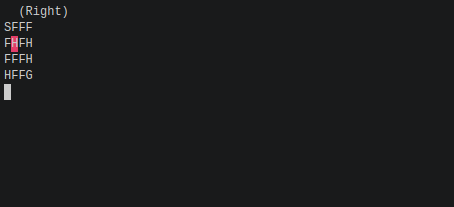
\includegraphics[width=0.5\textwidth]{frozen_lake.png}
%     \end{center}
%     \label{fig:frozen_lake2s}
% \end{figure}
%
Desenvolvido pela OpenAI, o \textit{Gym} [[1]] é, em sua essência, um conjunto
de simuladores de aprendizado por reforço que fornece ao pesquisador da área uma
série de cenários (chamados de \textit{environments}, ou ambientes) nos quais
seus algoritmos de aprendizado podem ser desenvolvidos e testados. Já havia,
antes da concepção do Gym, algumas outras ferramentas de \textit{benchmarking}
de AR, como o Arcade Learning Environment [[2]] ou o ViZDoom [[3]], mas, além de
reunir vários simuladores sob um único pacote, o Gym vai além e proporciona aos
desenvolvedores que usam sua plataforma uma maneira de publicarem seus
resultados, criando, desta forma, um ambiente colaborativo onde algoritmos
e soluções são compartilhados. O objetivo dos
idealizadores do Gym é criar, desta maneira, um ambiente onde desenvolvedores,
estudantes e pesquisadores colaborem entre si, ao invés de competirem,
encorajando que, junto com as soluções para cada problema, seja também fornecida
uma breve explicação de como o problema foi abordado, quais técnicas foram
usadas e como as informações fornecidas pelo ambiente foram interpretadas. Há
ainda a possibilidade de ser submetido, juntamente do código e do pequeno texto
explicativo, um vídeo ou imagem animada no formato \textit{gif} do problema
sendo resolvido, para ilustrar a evolução do treinamento e o resultado final
atingido.


A coleção de cenários ofecerida pelo Gym é bastante abrangente, contendo
problemas simples que podem ser descritos através de texto na tela do
\textit{console}, como  o problema chamado \textit{Frozen Lake}, retradado na
figura \ref{fig:frozen_lake}, até problemas que utilizam motores de física (como
o próprio MuJoCo, abordado na seção \ref{mujoco}) para representar intrincados
conjuntos de corpos e conexões. Por isso, não há apenas uma única maneira de
representar, por exemplo, um estado: cenários mais simples podem conter menos
informações a seu respeito ao mesmo tempo em que cenários que lidam com
problemas de robótica possuem muito mais dados os quais podem ser lidos durante
a fase de treinamento de um agente. Entretanto, todos os cenários do Gym foram
construídos com base em algumas diretrizes simples, que tentam uniformizar, no
que é possível, o processo de treinamento de um agente em um cenário
disponibilizado pelo Gym.


Apesar, todavia, de apresentar uma ampla coleção de problemas que, além de
possuírem uma estrutura padronizada, permitem que suas soluções sejam
compartilhadas, não há ferramentas que permitam a expansão desta coleção ou que
auxiliem na criação de cenários novos. Tal possibilidade, como discutida no
final da seção \ref{vizdoom_ale}, é primordial para o desenvolvimento de
algoritmos novos de aprendizado por reforço, uma vez que o desenvolvimento de
soluções novas requer também a construção de novas ferramentas comuns de
avaliação. Este trabalho apresenta uma ferramenta que auxilia na construção de
novos cenários de aprendizado por reforço que, além de compatíveis com motores
de física, também respeitam a estrutura ditada pelo \textit{Gym}.


% \chapter{Estado da Arte}
% [1] https://ieeexplore.ieee.org/abstract/document/7139807
% [2] https://ieeexplore.ieee.org/abstract/document/6386109
% [3] controller optimization => https://arxiv.org/abs/1509.01066
% [4] https://arxiv.org/pdf/1506.08941.pdf
% [5] VizDoom http://www.cs.put.poznan.pl/wjaskowski/pub/theses/ViZDoom_BScThesis.pdf
% [6] http://proceedings.mlr.press/v48/mniha16.pdf
% [7] https://arxiv.org/pdf/1707.02286.pdf
% [8] http://people.reed.edu/~jimfix/math385/lec01.1/Animation/p15-sims-evolving.pdf
% [9] http://ode.org/ode-latest-userguide.pdf

\chapter{Desenvolvimento}
\label{desenvolvimento}

% [1] Unity ML Agents-tk article

Conforme desenvolvido nos capítulos anteriores, técnicas de aprendizado por
reforço são aplicáveis a uma vasta gama de problemas, uma vez que existem
inúmeras situações onde problemas devem ser resolvidos através de uma sequência
de ações. Seja definir quais jogadas devem ser tomadas a fim de que uma partida
de um jogo de tabuleiro seja vencida ou decidir como regular a força propulsora
das hélices de um \textit{drone} autodirigido a fim de estabilizá-lo, quaisquer
problemas que requerem a tomada sequencial de ações e nos quais a qualidade
dessas ações seja captada pela noção de recompensa permitem o uso de técnicas de
aprendizado por reforço. Também foi extensamente discorrido e exemplificado
sobre a importância do uso de simuladores no treinamento de agentes de
aprendizado por reforço, mostrando que, apesar das diversas limitações que um
simulador pode possuir, tais ferramentas fornecem uma maneira poderosa de
modelar a abstração de um problema, deixando as diferentes situações às quais
o agente é submetido sob o controle daqueles que o treinam.


Além do papel imprescindível que ferramentas de modelagem de problemas de
aprendizado por reforço exercem durante a fase de treinamento de agentes para
resolvê-los, também foi discorrido acerca dos diferentes graus de especificidade
que tais \textit{softwares} podem apresentar. Para problemas de uma subárea
específica de aprendizado por reforço como a robótica, por exemplo, pode ser
mais vantajoso para quem deseja treinar um agente adotar ferramentas menos
genéricas de construção de ambientes em detrimento de ferramentas de propósito
mais geral, dado que \textit{frameworks} mais específicos fornecem atalhos para
a modelagem de problemas que não fogem ao seu escopo. Sendo assim, há de ser
analisado o \textit{trade-off} que surge do conflito entre a adoção de um
mecanismo de modelagem de simulações de propósito mais geral, que permite a
construção de problemas das mais variadas naturezas mas que não fornece atalhos
que facilitem a criação de simulações de uma área em específico, e a adoção de
ferramentas mais especializadas, como o \textit{Gazebo}, voltado para a
robótica, ou a \textit{Unity ML-Agents Toolkit}, voltada para problemas
envolvendo jogos onde agentes competem entre si, que fornecem caminhos mais
curtos e ferramentas que facilitam a criação de cenários dentro dos seus
próprios contextos.


Além da necessidade de haver programas de simulação com diferentes graus de
especificidade, também versamos neste trabalho sobre a necessidade de ter-se
meios comuns de avaliação de algoritmos: as chamadas ferramentas de
\textit{benchmark}. Tais mecanismos de avaliação de algoritmos fornecem uma base
comum de comparação para aqueles que propõem novos métodos de aprendizado por
reforço, permitindo que estes tenham sua performance facilmente posta à prova
quando aplicados em cenários ou problemas amplamente conhecidos e estudados.
Assim como apresentado na discussão acerca dos diferentes graus de
especificidade que um instrumento de simulação de problemas de aprendizado por
reforço pode ter, há aqui também um certo grau de limitação: como discutido em
[[1]], o desenvolvimento de novos algoritmos de AR depende diretamente do
constante criação de coleções de problemas de \textit{benchmark}, dado que tais
coleções tendem a tornarem-se praticamente inúteis à medida em que o campo do
aprendizado por reforço avança e os problemas fornecidos por elas são
resolvidos.


De todas as coleções de \textit{benchmark} analisadas por este trabalho, talvez
a mais famosa delas --- e certamente a que possui a coleção de problemas mais
ampla --- seja o \textit{framework} conhecido como \textit{Gym}. Muito mais do
que uma ferramenta de \textit{benchmark} com uma vasta coleção de diferentes
cenários que compreendem desde problemas simples, com representação em modo
texto, até problemas que envolvem robôs que devem aprender a andar em universos
virtuais regidos por um motor de física, \textit{Gym} consegue ir além e
fornecer meios de compartilhamento de soluções para os problemas oferecidos,
estimulando a colaboração entre pesquisadores do mundo todo.


Apesar da vasta coleção oferecida pelo \textit{Gym} e pela facilidade com que
diferentes soluções para um mesmo problema podem ser comparadas e
compartilhadas, há poucas ferramentas disponíveis para a a criação e o
compartilhamento de cenários novos. A criação de cenários novos para ferramentas
de \textit{benchmark} é tão importante quanto o desenvolvimento de novos métodos
de aprendizado, apesar de não receber tanta atenção por parte dos especialistas
como a construção de novos algoritmos. O campo carece, portanto, de uma
ferramenta que permita o desenvolvimento rápido de novos cenários para a
expansão de coleções de \textit{benchmark}.


Este trabalho é uma tentativa de estabelecer um meio para a criação de novos
cenários de aprendizado por reforço. Além de fornecer um meio simples para a
modelagem de problemas de qualquer natureza, tentando, quando possível, agregar
elementos presentes em ferramentas de simulação de alto grau de especificidade e
que funcionam como atalhos na criação de cenários, o trabalho aqui desenvolvido
produz cenários compatíveis com a API do \textit{Gym}, beneficiando-se, desta
maneira, das ferramentas disponibilizadas pela plataforma para o
compartilhamento, a avaliação e a comparação de diferentes soluções para um
mesmo problema.


O \textit{Barbell}, \textit{software} proposto por este trabalho, é, portanto,
uma espécie de extensão ao \textit{Gym}, que permite que sua coleção de
problemas seja expandida através de ferramentas que visam facilitar a construção
de novos cenários de aprendizado por reforço. Ao mesmo tempo que tenta empregar
as vantangens oferecidas por simuladores altamente específicos, como a descrição
textual de elementos a serem simulados no ambiente, o \textit{Barbell} tenta
manter a natureza genérica do \textit{Gym}, aplicando, desta maneira, as
vantagens de simuladores de alto grau de especificidade na modelagem de
problemas das mais diversas naturezas.


A seguir, o funcionamento do \textit{Gym} será estudado de maneira detalhada, a
fim de que suas funções sejam compreendidas. Logo após, as funcionalidades do
\textit{Barbell} serão apresentadas a fim de que fique claro para o leitor
quais funcionalidades são estas e de que maneira elas se beneficiam daquilo
que o \textit{Gym} já fornece.



\section{Objetivo do Gym}
% [1] - https://www.nature.com/news/1-500-scientists-lift-the-lid-on-reproducibility-1.19970



Conforme descrito na seção \ref{sec:gym}, \textit{Gym} é uma ferramenta que
apresenta uma coleção de modelagens de problemas de aprendizado por reforço
(chamadas de \textit{cenários}) e que é mantida pela OpenAI, uma entidade sem
fins lucrativos que promove estudos na área de inteligência artificial e cujo
intuito é "desenvolver IA amigável de tal forma que a humanidade como um todo
beneficie-se dela". Seu trabalho com o \textit{Gym}, portanto, não tem por
objetivo somente fornecer a pesquisadores do mundo todo uma ferramenta com a
qual seja possível desenvolver, avaliar e comparar diferentes algoritmos de
aprendizado por reforço, mas também fornecer a todos que usam os simuladores do
\textit{Gym} um canal por onde se possa compartilhar ideias e comparar métodos.


É inegável que o compartilhamento de conhecimento entre pesquisadores de uma
determinada área é essencial para alavancar o seu desenvolvimento. Entretanto, a
escolha do canal ou da forma através dos quais este conhecimento é compartilhado
pode muitas vezes limitar o seu alcance ou até mesmo impedir por completo que
experimentos sejam replicados. O problema da reprodutibilidade é bastante
conhecido: em uma pesquisa conduzida pela revista Nature [[1]], 70\% dos
pesquisadores entrevistados admitiram que, ao menos uma vez, já tentaram, sem
sucesso, reproduzir os experimentos de artigos escritos por terceiros, e mais da
metade dos entrevistados disseram ter tido dificuldades em reproduzir os
próprios experimentos. Do mesmo modo, também podem residir limitações no canal
escolhido para divulgar um estudo novo: a grande maioria dos periódicos de
artigos científicos é paga, o que pode vir a afastar o conhecimento daqueles que
não têm dinheiro suficiente para pagar por ele.


\begin{figure}[h]
    \caption{Classificação das melhores soluções para o problema
    \textit{Mountain Car}.}
    \begin{center}
      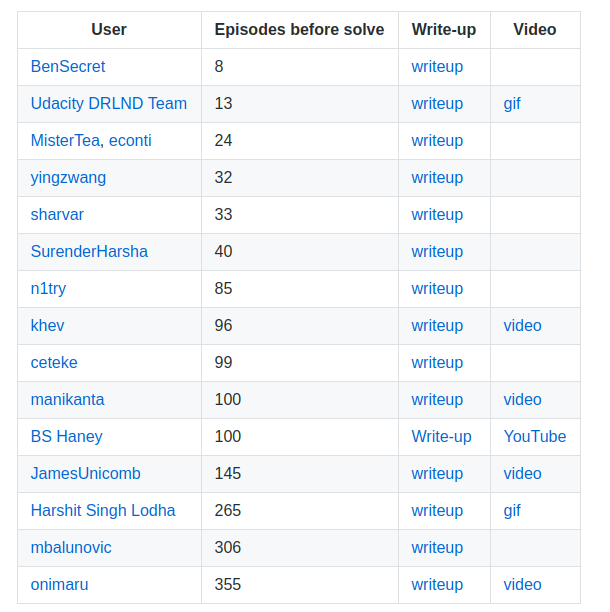
\includegraphics[width=0.6\textwidth]{leaderboard.png}
    \end{center}
    \label{fig:leaderboard}
\end{figure}


Residem problemas, portanto, na forma com que o conhecimento derivado de estudos
novos é passado adiante: nem sempre um artigo científico apresenta experimentos
de fácil reprodução e nem sempre ele é publicado em um canal de fácil acesso ao
grande público. Há uma tentativa, entretanto, por parte dos responsáveis pelo
\textit{Gym}, de atenuar este problema: ao estimular que soluções para os
cenários oferecidos por ele sejam publicadas em um espaço aberto na rede, o
acesso a algoritmos avançados de aprendizado por reforço é democratizado. A
maneira através da qual o \textit{Gym} propicia este compartilhamento de
soluções é bem simples: há um guia, no formato de uma enciclopédia
\textit{on-line} e editável, que lista todos os cenários oferecidos pelo
\textit{Gym}, juntamente com as soluções de melhor performance. Há duas maneiras
diferentes de se medir a performance de uma solução, de acordo com o cenário:
em alguns cenários, o critério que qualifica as soluções é o numero de épocas de
decisão necessárias para que o agente pudesse solucionar o problema --- e aqui
a definição de "solução" é particular de cada cenário: no problema chamado de
\textit{Cart Pole}, por exemplo, o problema é considerado solucionado quando a
recompensa acumulada de um episódio ultrapassa uma determinada marca --- e em
outros problemas, estes mais complexos e, portanto, mais difíceis de definir
quando o problema foi de fato solucionado, usam como critério de avaliação de
soluções apenas a recompensa média recebida em cem episódios. Os números são
facilmente verificáveis, uma vez que, juntamente com um pequeno texto que
explica o funcionamento do algoritmo, deve ser também submetido o código
utilizado na solução, com ambos ficando disponíveis para \textit{download}. Em
alguns casos, também é encorajada a submissão de um vídeo ou imagem no formato
\textit{GIF} do comportamento do agente, quando da solução do problema. Um
exemplo de listagem das melhores soluções para um problema da coleção do
\textit{Gym} é dado na figura \ref{fig:leaderboard}.


\section{Implementação do Gym}

Além de atacar o problema resultante da dificuldade em compartilhar-se
resultados de um experimento, o \textit{Gym} propõe uma espécie de padronização
de problemas de aprendizado por reforço, que fica evidente quando é analisada a
maneira através da qual os diferentes problemas de aprendizado por reforço são
transformados em cenários do \textit{Gym}. Na seção a seguir, será estudada a
implementação do \textit{Gym}, para que fique claro de que maneira esta
padronização é feita.


\subsection{Representação do ciclo de aprendizado}
% [1] - R. S. Sutton and A. G. Barto. Reinforcement Learning: An Introduction. MIT Press, 1998
% [2] - http://citeseerx.ist.psu.edu/viewdoc/download?doi=10.1.1.146.1515&rep=rep1&type=pdf
A implementação do \textit{Gym} é bastante próxima do ciclo de aprendizado de um
agente de AR definido na imagem \ref{fig:fluxo_ar}, baseando-se apenas nos
seguintes conceitos de aprendizado por reforço:

\begin{itemize}
  \item o agente está inserido em um ambiente;
  \item a cada passo, o agente toma uma \textit{decisão} e recebe uma
        \textit{recompensa} e realiza uma \textit{observação} do ambiente;
  \item o ambiente é representado através de Processo de Decisão de Markov
  Parcialmente Observável (POMDP) [[1]].
\end{itemize}

Baseando-se nos conceitos acima, o grande destaque do \textit{Gym} talvez seja
no sistema de \textit{episódios} de um treinamento de uma gente de AR. Quando um
treinamento de um agente separa-se em episódios, um cenário é iniciado em um
estado randômico e o agente toma uma série de decisões até que uma ação
modifique o ambiente de tal forma que ele transicione para um estado terminal.
Quando isso ocorre, é calculada a recompensa total, acumulada durante toda a
sequência de ações tomadas pelo agente desde o momento em que o cenário foi
inicializado até o momento em que ele chegou em um estado terminal, e o cenário
é reinicializado.
O código a seguir exemplifica a inicialização de um agente, que toma uma série
de ações até que um estado final seja atingido:

\begin{minted}[linenos]{python}
  # definição do cenário
  env = gym.make('CartPole-v0')

  # cenário é inicializado, observação retornada
  obs = env.reset()
  done = False

  while not done:
    # observação, recompensa para a ação tomada
    # e variável booleana indicando se cenário
    # chegou a um estado terminal são retornados
    obs, reward, done = env.step(agent.act(observation))
\end{minted}

É necessário observar aqui que toda a modelagem de um cenário disponibilizado
pelo \textit{Gym} gira em torno do ambiente e das transições entre seus estados.
O agente, apesar de ser um conceito bastante importante em problemas de
aprendizado por reforço, não possui uma abstração explícita no \textit{Gym} (no
exemplo acima, um agente, desenvolvido à parte, age de acordo com a observação),
permitindo, desta maneira, que ele seja modelado da maneira que for mais
conveniente para quem desenvolve soluções para um determinado cenário. Toda
informação relevante para a solução do problema é retornada durante uma tomada
de decisão (exemplificada na linha 12 do código acima) e segue o formato
$(observation, reward, done, info)$, onde:

\begin{itemize}
  \item $observation$ é um vetor de números que representa o estado do ambiente
  naquele momento;
  \item $reward$ é a recompensa atribuída à ação tomada;
  \item $done$ é uma variável binária que diz se o estado atual do ambiente é
  um estado terminal, utilizada para reiniciar as simulações quando assim for
  conveniente;
  \item $info$ é um dicionário com informações adicionais sobre o episódio,
  utilizado apenas quando necessário.
\end{itemize}

Este formado, através do qual as informações do cenário são representadas,
juntamente com a ausência de uma abstração da entidade tomadora de decisões,
permite vários estilos diferentes de aprendizado. As informações retornadas a
cada $n$ episódios, por exemplo, podem ser agrupadas em um lode de dados que
só mais tarde, após finalizados os episódios, é repassado a uma entidade de
aprendizado por reforço que processa as informações e atualiza o seu agente de
acordo. Um outro estilo de aprendizado, por exemplo, pode consistir em utilizar
as informações de cada episódio para o treinamento do agente no momento em que
elas são fornecidas, corrigindo o seu comportamento de maneira incremental. Além
disso, a ausência de um modelo de agente permite que sejam desenvolvidos
cenários onde dois ou mais agentes atuam.


A decisão de subtrair do sistema a abstração de um agente, portanto, dá mais
liberdade para pesquisadores desenvolverem agentes com a interface que for mais
conveniente. Com o agente transformado em uma espécie de "caixa-preta" no
ecossistema do \textit{Gym} é bastante simples que diferentes agentes sejam
utilizados alternadamente a fim de que suas performances sejam comparadas
utilizando-se de um mesmo cenário de base. É possível também que um agente seja
pré-treinado em um problema antes de ser inserido em outro cenário, permitindo
que o conhecimento adquirido no primeiro cenário seja utilizado no segundo,
técnica conhecida como \textit{transfer learning} [[2]].

\section{Representação dos resultados}

\begin{figure}[h]
    \caption{Classificação das melhores soluções para o problema
    \textit{Pendulum-v0}.}
    \begin{center}
      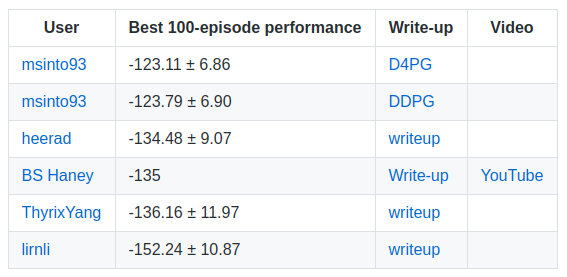
\includegraphics[width=0.6\textwidth]{leaderboard_best100.png}
    \end{center}
    \label{fig:leaderboard_best100}
\end{figure}

Além de versar sobre a forma como os cenários são representados no \textit{Gym},
é importante também falar sobre como os resultados de um treinamento são
gravados. A performance de um treinamento pode ser medida de acordo com dois
critérios: o primeiro é a quantidade de episódios necessários para que o
problema seja dado como resolvido, critério este que varia de acordo com o
cenário. Nem todos os cenários, entretanto, possuem um mecanismo que informa
explicitamente se o problema foi resolvido; há, portanto, um meio alternativo
de se medir a performance de um treinamento: usa-se, neste caso, os melhores
valores de recompensas totais recebidas para uma série de cem episódios
consecutivos, como ilustrado na figura \ref{fig:leaderboard_best100}.
Para que seja facilitada a comparação de resultados, o \textit{Gym} possui
uma estrutura interna chamada de \textit{Monitor}, que mantém um controle
interno de todas as vezes que o uma simulação é atualizada ou reiniciada. Esta
estrutura, que também pode gravar videos periodicamente, torna possível a
construção de curvas de aprendizado, a partir dos dados oriundos das
recompensas recebidas. O código a seguir ilustra uma situação onde o
\textit{Gym} é programado para gravar vídeos do treinamento em uma pasta chamada
\textit{recording}.

\begin{minted}[linenos]{python}
  env = gym.make("CartPole-v0")
  env = gym.wrappers.Monitor(env, "recording")
\end{minted}


\textit{Arquitetura de um cenário}
Depois de explicitados os meios através dos quais o \textit{Gym} representa as
informações do ambiente, como o agente lê essas informações e como os resultados
do seu aprendizado são arquivados para análises futuras, resta saber como um
cenário é modelado no sistema do \textit{Gym}. Primeiro, algumas definições são
necessárias: um \textit{módulo} nada mais é do que uma coleção de funções que
possuem uma finalidade específica, enquanto um \textit{pacote} é uma coleção de
módulos e de outros subpacotes. Em \textit{Python}, um pacote é representado por
uma pasta, enquanto módulos são representados por arquivos. Caso queiramos
definir um pacote chamado \textit{generic\_package}, que contém dois módulos
\textit{a} e \textit{b}, portanto, devemos definir em um sistema a estrutura de
arquivos representada na figura \ref{fig:python_package}. O arquivo
\textit{\_\_init\_\_.py} é obrigatório e serve para marcar para o motor da
linguagem que aquela pasta representa um pacote.

\begin{figure}[h]
  \label{fig:python_package}
  \caption{Estrutura de um pacote na linguagem \textit{Python}}
  \vspace{2mm}
  \begin{center}
    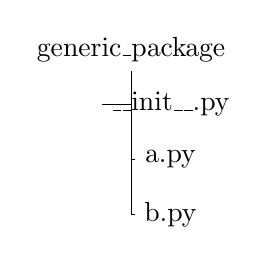
\begin{tikzpicture}[%
      grow via three points={one child at (0.5,-0.7) and
      two children at (0.5,-0.7) and (0.5,-1.4)},
      edge from parent path={(\tikzparentnode.south) |- (\tikzchildnode.west)}]

      \node {generic\_package}
          child { node {\_\_init\_\_.py}}
          child { node {a.py}}
          child { node {b.py}};

    \end{tikzpicture}
\end{center}
\end{figure}

Caso o pacote siga a estrutura da figura \ref{fig:python_package}, ele pode ser
incluído em um \textit{script Python} da seguinte maneira:

\begin{minted}[linenos]{python}
  import generic_package
  from generic_package import a, b
\end{minted}

Um cenário pertencente ao \textit{Gym} segue a estrutura de um pacote
\textit{Python}, com a exceção de que, como um cenário agrupa mais de um pacote
em sua estrutura, ela é ligeiramente mais complexa do que a apresentada na
figura \ref{fig:python_package}. Caso queiramos, portanto, definir um cenário
chamado \textit{rl\_problem} que contenha duas versões, \texttt{rl\_problem-v0}
e \texttt{rl\_problem\_hard-v0}, todo: continuar

\section{Implementação do Barbell}
\blindtext[2]
%
% É inegável que o compartilhamento de conhecimento entre pesquisadores da área é
% essencial para alavancar o seu crescimento. O canal para este compartilhamento,
% entretanto, muitas vezes é

 - compartilhamento de soluções
 - wiki... video ou gif
 - reprodutibilidade
 - T R A N S F E R    L E A R N I N G

 - Como o gym define o bagulho la do ciclo
 - renderizaçao

 - barbell

%
% Gym é um simulador desenvolvido pela OpenAI \bruno{nao é um simulador. É uma API},
% uma empresa sem fins lucrativos que desenvolve pesquisas em inteligência artificial com o intuito de
% "desenvolver IA amigável de tal forma que a humanidade como um todo beneficie-se dela". Seu trabalho com o Gym, portanto, não tem por objetivo
% somente prover a pesquisadores do mundo todo uma ferramenta com a qual seja possível
 % desenvolver, \bruno{avaliar e comparar diferentes} algoritmos de aprendizado por reforço, mas também
% fornecer a todos que usam o simulador um canal por onde se possa compartilhar
% ideias e comparar métodos. O Gym nasceu, portanto, da necessidade de
% se ter uma ferramenta capaz de fazer o \textit{benchmark} de algoritmos de AR.
 % Enquanto em outras áreas da IA, como aprendizado supervisionado,
% já existe grandes bases de dados como a ImageNet, com centenas de milhares de imagens já etiquetadas para
% uso principalmente em projetos de IA que
% envolvam reconhecimento de imagens, não existia, até o momento em que o Gym
% foi concebido, uma biblioteca de ambientes e resultados que fosse grande
% o suficiente e que, principalmente, fosse fácil de usar
\bruno{tem que clarificar que é uma API que tu usa pra especificar tanto os
ambientes de RL quanto os algoritmos de aprendizado, e que como toda a interface
 fica padronizada, é possivel fazer combinacoes e testar qualquer algoritmo em
  qualquer ambiente, e é possível reproduzir resultados de outros algoritmos,
  facilmente comparar novos algoritmos com aqueles existentes, etc. Aí precisa
  dizer concretamente o que o Gym faz: qual a interface de métodos principais
  que a pessoa precisa implementar pra especificar um ambiente, e quais precisa
   implementar pra especificar um agente de aprendizado. Diz aí tipo 'o metodo
   takeAction, p.ex., implementa a politica $\pi$ de escolha de acoes. O metodo
   runAction (to inventendo os nomes, nao lembro de cor) pega uma acao e o
    estado atual, e devolve o proximo estado do ambiente e a recompensa; ou
    seja, ele corresponde à implementacao computacional da funcao de transicao
    T do MDP e da funcao de recompensa R'. Acho que falta, nessa parte, falar
    de forma mais concreta o que que é o que o Gym faz/especifica, pra conseguir
     fazer essa padronizacao. Isso é importante porque todo o teu argumento,
     depois, é que o teu framework, ao gerar codigo compativel com o Gym,
     permite a geracao facilitada de novos ambientes para teste, avaliacao
      e comparacao de algoritmos de RL. Quando for explicar o Gym, tu poderia
      nao só colocar aquelas imagens, mas realmente descrever alguns deles,
      como exemplos. Tipo 'Alguns exemplos de ambientes clássicos usados
      como benchmark de algoritmos de aprendizado por reforco, tais como
      poll balancing e mountain car, por exemplo, estao disponiveis na
      plataforma Gym. O mountain car corresponde ao problema de (...).
      Para que um desenvolvedor com interesse em implementar e validar
       um novo algoritmo de RL pudesse testar sua criacao no mountain
       car, bastaria utilizar o seguinte codigo Python: (...).
       Caso quisesse testar esse metodo codigo no problema de poll
       balancing, bastaria alterar o codigo do seu agente de aprendizado
        da seguinte forma: (...). Como pode ser visto, uma vez que
         ambientes e agentes sao implementados seguindo a API do Gym,
          torna-se trivial instanciar comparacoes de qualquer método em
          qualquer tarefa de aprendizado'. Aí fala 'alem de ambientes
          classicos, cenarios mais recentesmente propostos como benchmark,
          tais como aqueles envolvendo jogos de atari, tambem estao
           disponiveis'. Aí fala um pouco deles. Depois de falar sobre a
           parte de cenarios/ambientes que tem no Gym, fala sobre como é
           sao disponibilizados os algoritmos de aprendizado que existem
           nele. As pessoas enviam codigo pra resolver um ambiente especifico,
            e o codigo é rodado la? Elas rodam localmente e loggam os resultados,
             e só os resultados sao enviados, com alguma maneira de eles
             verificarem que nao foram adulterados? Tem alguma maneira facil
             de baixar os top N best-ranked algorithms pra um detemrinado
             problema? Coisas desse tipo. Aí descreve como ter acesso aos melhores algoritmos submetidos pra um dado ambiente é util pra que depois tu possa pegar o algoritmo que tu inventou e comparar com o estado-da-arte, de acordo com as pessoas que submetem pro Gym; fala que esse ranking é interessante porque consiste em resultados que podem ser reproduzidos, e nao apenas em resultados que *apenas* foram publicados em artigos cientificos, mas para os quais frequenemtenete nao se tem acesso ao fonte, e/ou nao se conhece como os autores ajustaram os meta-parametros tipo taxa de aprendizado, etc. Ou seja, facilidade reproducibility e permite com que tu rapidamente avalie o teu algoritmo contra varios existentes, ou entao teste algoritmos existentes (publicados la) em um novo tipo de ambiente/tarefa de aprendizado, no qual tu possa ter interesse}.\par
%
% Os cenários disponibilizados pelo Gym são bastante diversos e vão desde problemas em modo texto até jogos de plataformas bidimensionais (figura \ref{fig:gymenvironments}).
% Para cada um dos \textit{enviroments} disponíveis, há, na página do projeto, um \textit{ranking} dos algoritmos que resolveram o problema da maneira mais eficiente,
% levando dois fatores em consideração: maior recompensa recebida e quantidade de episódios necessários para que o agente finalmente resolvesse o problema proposto.
% Todavia, o Gym ainda carece de uma extensão que permita que pesquisadores compartilhem não só suas soluções, mas também ambientes totalmente novos ou adaptações
% de ambientes que já existem \bruno{o que tu quer dizer com isso é que o pacote, como tu baixa da pagina, vem só com um conjunto pre-aceito de ambientes, ne? Que as pessoas tem como submeter seus agentes de aprendizado, mas nao seus ambientes? Isso é uma limitacao importante? Nao poder compartilhar os ambientes, digo? Porque caso tu enfatize essa limitacao, a expectativa do leitor seria que tu iria resolver ela (uma plataforma pra poder submeter novos ambinetes). Acho que a tua contribuicao nao é essa, e sim resolver uma outra limitacao dele: que ele especifica só a API, mas aí se tu quer criar um ambiente novo do zero, que siga a API deles, tu precisa ir aprender uns motor de fisica do zero, e tambem precisa aprender a API da plataforma e tudo mais. O que tu vai fazer é propor um framework pra geracao automatica de codigo que pegue a especificacao de alto-nivel de um ambiente e compile ela pra codigo de mais baixo nivel que implementa essa descricao em um motor de fisica, e de forma que tudo seja compativel com Gym, ou seja, de forma que instantaneamnete dê pra disponbilizar pra toda comunidade esse novo ambiente, e que se instantanemanete tenha acesso/possibilidade de avaliar N algoritmos existentes no ambiente que tu acabou de inventar}.
%
% O \textit{Barbell}, desenvolvido e descrito neste trabalho, é uma tentativa de resolver, mesmo que em partes, este problema: ao
% fornecer ao desenvolvedor uma maneira de criar seus próprios ambientes, cria-se a possibilidade de expandir a biblioteca do Gym; por outro lado, ao desenvolver
% cenários que de certa forma recordem outros que já existem, o \textit{Barbell} permite que o desenvolvedor parta de algoritmos que já foram desenvolvidos ao
% invés de se encontrar obrigado a construir sua solução do zero. O método de construção de cenários e a maneira como os resultados são apresentados, em comparação
% com os resultados fornecidos pelos cenários padrão do Gym, será descrito no próximo capítulo.


% \subsection{Ciclo de aprendizado no Gym}
% \blindtext
% \section{Barbell}
% \blindtext[2]

% Apesar da vasta coleção oferecida pelo \textit{Gym} e pela facilidade com que
% diferentes soluções para um mesmo problema podem ser comparadas e
% compartilhadas, há poucos meios disponíveis de criar-se e compartilhar-se

% \label{estadodaarte}





\begin{figure}[h]
    \caption{Alguns dos cenários disponíveis na base do Gym.}
    \begin{center}
      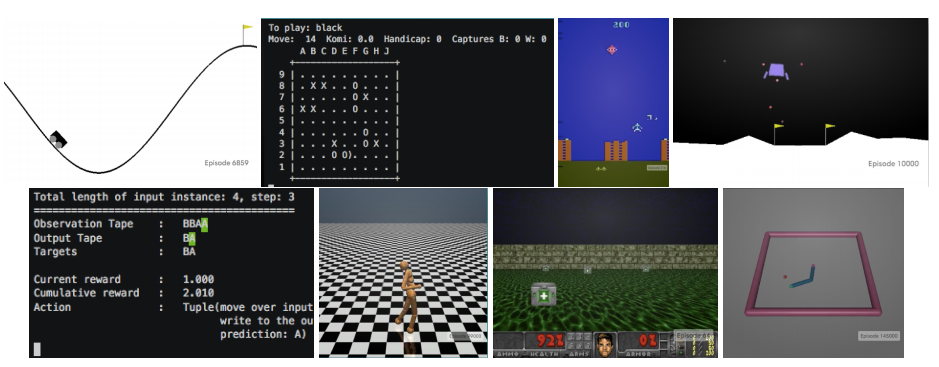
\includegraphics[width=0.9\textwidth]{environments.png}
    \end{center}
    \label{fig:gymenvironments}
\end{figure}


\section{MuJoCo}

\bruno{\textbf{IMPORTANTE}: que outros artigos discutem frameworks com esse mesmo objetivo? DISCUTIR ISSO NOS TRABALHOS RELACIONADOS:
\begin{itemize}
    \item rllab, moveit \url{https://stackoverflow.com/questions/48490828/should-i-using-mujoco-or-moveit-for-modeling};
    \item quais outros motores de fisica as pessoas usam? gazebosim.org, vrep;
    \item como as pessoas implementam os dominios compativeis com o RLGlue?
    \item que outros simuladores de robotica sao utilizados? p.ex. \url{https://en.wikipedia.org/wiki/Robotics_simulator};
    \item andersonrochatavares@gmail.com, perguntar se ele conhece artigos e/ou frameworks que se costuma usar para gerar jogos/dominios;
\end{itemize}
}


\bruno{ver comentario no inicio do capto. Acho que o gym e o mujoco nao sao comparaveis, porque Gym=API, e mujoco=framework pra geracao de ambientes/simulacoes. ALgo comparavel com mujoco seriam aqueles outros trabalhos que eu mencionei em algum dos emails anteriores}

\chapter{Desenvolvimento}
\label{desenvolvimento}

% [1] gym => https://arxiv.org/pdf/1606.01540.pdf
% [2] ALE => https://www.jair.org/index.php/jair/article/view/10819
% [3] ViZDoom, já mencionado antes

Neste capítulo, serão indicadas as razões por trás do desenvolvimento do
Barbell, a fim de justificar sua criação. A seção \ref{sec:gym} traz um breve
panorama sobre a plataforma \textit{Gym}, explicitando suas maiores qualidades e
suas deficiências mais evidentes. A seção seguinte trará, por sua vez, uma breve
exposição dos pontos do Barbell no qual ele supre as principais carências do
Gym e também discursará a respeito das principais decisões de \textit{design}
tomadas durante o desenvolvimento do \textit{software}.

\section{Gym}
\label{sec:gym}

\begin{figure}[h]
    \caption{Modelagem de robôs humanoides no ambiente do MuJoCo}
    \begin{center}
      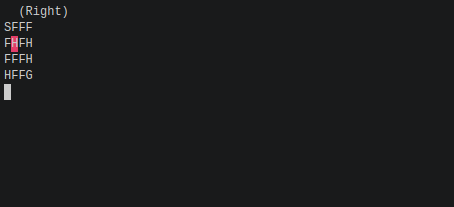
\includegraphics[width=0.5\textwidth]{frozen_lake.png}
    \end{center}
    \label{fig:frozen_lake2s}
\end{figure}

Desenvolvido pela OpenAI, uma organização sem fins lucrativos voltada para o
estudo na área de inteligência artificial e para as formas através das quais a
sociedade pode beneficiar-se deste conhecimento, o \textit{Gym} [[1]] é, em sua
essência, um conjunto de simuladores de aprendizado por reforço que fornece ao
pesquisador da área uma série de cenários (chamados de \textit{environments}, ou
ambientes) nos quais seus algoritmos de aprendizado podem ser desenvolvidos e
testados. Já havia, antes da concepção do Gym, algumas outras ferramentas de
\textit{benchmarking} de AR, como o Arcade Learning Environment [[2]] ou o
ViZDoom [[3]], mas, além de reunir vários simuladores sob um único pacote, o Gym
vai além e proporciona aos desenvolvedores que usam sua plataforma uma maneira
de publicarem seus resultados, criando, desta forma, um ambiente
colaborativo onde algoritmos e soluções são compartilhados. O objetivo dos
idealizadores do Gym é criar, desta maneira, um ambiente onde desenvolvedores,
estudantes e pesquisadores colaborem entre si, ao invés de competirem,
encorajando que, junto com as soluções para cada problema, seja também fornecida
uma breve explicação de como o problema foi abordado, quais técnicas foram
usadas e como as informações fornecidas pelo ambiente foram interpretadas. Há
ainda a possibilidade de ser submetido, juntamente do código e do pequeno texto
explicativo, um vídeo ou imagem animada no formato \textit{gif} do problema
sendo resolvido, para ilustrar a evolução do treinamento e o resultado final
atingido.


A coleção de cenários ofecerida pelo Gym é bastante abrangente, contendo
problemas simples que podem ser descritos através de texto na tela do
\textit{console}, como  o problema chamado \textit{Frozen Lake}, retradado na
figura \ref{fig:frozen_lake}, até problemas que utilizam motores de física (como
o próprio MuJoCo, abordado na seção \ref{mujoco}) para representar intrincados
conjuntos de corpos e conexões. Por isso, não há apenas uma única maneira de
representar, por exemplo, um estado: cenários mais simples podem conter menos
informações a seu respeito ao mesmo tempo em que cenários que lidam com
problemas de robótica possuem muito mais dados os quais podem ser lidos durante
a fase de treinamento de um agente. Entretanto, todos os cenários do Gym foram
construídos com base em algumas diretrizes simples, que tentam uniformizar, no
que é possível, o processo de treinamento de um agente em um cenário
disponibilizado pelo Gym.


\subsection{Representação de um cenário}
Toda a modelagem de um cenário disponibilizado pelo Gym gira em torno do
cenário. O agente, outro conceito fundamental de um problema de aprendizado por
reforço, não possui uma abstração explícita no Gym, permitindo, desta maneira,
que o agente seja modelado da maneira que for mais conveniente para os usuários
da plataforma. As informações referentes ao estado do ambiente, fornecidas a
cada episódio de aprendizado, seguem o formato $(observation, reward, done)$,
onde:

\begin{itemize}
  \item $observation$ é um vetor de números que representa o estado do ambiente
  naquele momento;
  \item $reward$ é a recompensa atribuída à ação tomada no episódio anterior;
  \item $done$ é uma variável binária que diz se o estado atual do ambiente é
  um estado terminal, utilizada para reiniciar as simulações quando assim for
  conveniente.
\end{itemize}

Este formato através do qual as informações do cenário são representadas,
juntamente com a ausência de uma abstração da entidade tomadora de decisões,
permite vários estilos diferentes de aprendizado. As informações retornadas a
cada $n$ episódios, por exemplo, podem ser agrupadas em um lote de dados que só
mais tarde, após finalizada a época de treinamento (ou seja, após o sistema
entrar em um estado terminal), é repassado a uma entidade de aprendizado por
reforço que processa as informações e atualiza seu agente de acordo. Um outro
estilo de aprendizado, por exemplo, pode consistir em utilizar as informações de
cada episódio no momento em que elas são fornecidas, corrigindo o comportamento
do agente de maneira incremental.

\subsection{Representação dos resultados}
É importante que seja explicitada a forma com que os resultados submetidos para
algum cenário fornecido pelo Gym são representados e avaliados: na grande
maioria dos casos, a performance de uma solução pode ser medida de acordo com
dois critérios. O primeiro é a recompensa total recebida pelo agente, após o seu
treinamento, ao mesmo tempo que o segundo critério é o tempo, medido em número
de épocas de decisão, que o treinamento levou para fazer com que o agente tenha
atingido sua performance máxima. A maneira com que é decidido se o treinamento
já atingiu o comportamento esperado para um agente, entretanto, depende bastante
do cenário que está sendo trabalhado, sendo esta decisão tomada de uma maneira
bastante ligada ao problema abordado, não havendo um método generalizado para
este tipo de decisão.


Para que seja facilitada a comparação de resultados, cada cenário do Gym possui
uma estrutura interna chamada de \textit{Monitor}, que mantém um controle
interno de todas as vezes que o uma simulação é atualizada ou reiniciada. Esta
estrutura, que também pode gravar videos periodicamente, torna possível a
construção de curvas de aprendizado, quando combinada com os dados oriundos das
recompensas recebidas.

\section{Daqui pra baixo é lixo}

Realmente não sei o que colocar aqui. Acho que tenho que convencer nessa parte de que meu trabalho é muito mais foda e muito
mais intuitivo do que todos os outros trabalhos que já foram desenvolvidos até hoje, certo?
Bruno, por favor, me ajuda.
\bruno{Aqui precisa descrever algo como o que eu tinha mencionado numa thread de emails com subject 'TODO + exemplo de TCC', e também ao longo da thread com subject 'TCC. estou desesperado'. Fala do que tu fez, qual a sintaxe da linguagem de alto nivel que tu criou, o que tu consegue especificar com ela, como tu especifica as propriedades fisicas do agente, as acoes que ele pode executar, a funcao de recompensa, etc. Fala como tu faz pra pegar esse negocio e compilar pra codigo de mais baixo nivel usando um motor de fisica. Diz como tu escolheu essa sintaxe especifica, ou seja, porque tu nao fez uma coisa mais geral (mas mais dificil de usar), tipo mujoco. Pra fazer isso tu pode fazer um link com o que falou antes, na secao do mujoco, onde tu fala que ele é super generico mas é de dificil uso pra leigos, que tem uma curva acentuada de aprendizado, etc, e que aqui tu foca em poder criar ambientes que tenham essa estrutura de um jogo, que é o que acontece na imensa maioria dos ambientes existentes em benchmarks padroes da area e dentre os ambientes no Gym. Fala de como tu organizou o teu codigo, quais metodos da API do Gym ele implementa automaticamente, quais ele implementa parcialmente mas deixa o usuario completar com codigo mais refinado (tipo a definicao de novas acoes, ou a definicao da funcao de recompensa). A gente tinha conversado tambem sobre aquela questao de haver N sensores no ambiente/agente, e aí ter uma funcao que calcula o estado, que vai ser um subset desses sensores (e/ou novos valores calculados com base neles), e que vai ser efetivamente o que vai ser usado para escolher acoes, etc. Fala como isso funciona. Esse tipo de coisa}


Neste capítulo, será mostrado o funcionamento dos mecanismos fornecidos pelo Barbell para a modelagem de ambientes e agentes que nele operam, bem como uma
visão geral sobre a sua estrutura básica, com uma breve explicação das diferentes partes do seu mecanismo e quais os papéis desempenhados por cada uma delas. Após
finalizar a leitura deste capítulo, o leitor será capaz de criar seus próprios problemas de AR usando qualquer um dos dois conjuntos de ferramentas de criação
disponibilizados pelo Barbell: o leitor de \textit{scripts}, YAML que lê um arquivo com uma descrição textual da estrutura do problema \bruno{de aprendizado/ambiente (incluindo a especificação da dinânamica do ambiente, estrutura física do agente, ações disponíveis ao agente, e função recompensa)}, ou as funções
disponibilizadas pela API do projeto Barbell, que, se chamadas diretamente, executam as mesmas funções.
Todas as entidades envolvidas em um problema de AR (como o agente e as partes que o compõem, bem como o ambiente e seus objetos) podem ser criados através
da chamada de comandos específicos fornecidos pela API ou através de um \textit{script} escrito em YAML, que define a estrutura do projeto (sob o formato
de uma estrutura que combina vetores associativos e listas de elementos, como explicado na seção \ref{alinguagemyaml} \bruno{essa parte está confusa. O que tu quer dizer com projeto, exatamente? é a especificacao de um ambiente especifico? o conjunto de arquivos necessarios pra fazer isso? é o script yaml? nao definiu o que signfica projeto. A descricao de que é implementado com vetores associativos e listas tambem ta detalhada demais e fora de lugar, aqui nessa etapa do texto, aonde tu ainda ta recebem comecando a explicar o que é. O leitor nem sabe direito o que tu fez e tu ta explicando que internamente é um vetor associativo}) e as informações
a respeito de todas as partes que cumprem algum papel na simulação. Neste capítulo, portanto, será dada uma breve \bruno{porque breve? esse é o capto principal} explicação sobre a estruturação de um projeto \bruno{projeto=ambiente?}
utilizando-se do \textit{framework} Barbell, bem como quais comandos devem ser executados (ou quais linhas devem ser incluídas no \textit{script}) para que sejam criados
o agente, o ambiente e todas as demais partes do problema.
\section{Características básicas do funcionamento sistema}

\subsection{Ciclo de aprendizado}
O sistema \bruno{qual sistema? o barbell implementa esse ciclo? ou ele gera ambientes com os quais um agente de AR pode interagir, ao ser utilizado (por outros softwares) numa tarefa de aprendizado que siga esse ciclo?} segue o formato do ciclo de aprendizado via interação com o ambiente descrito na figura \ref{fig:fluxo_ar}. No início de cada episódio, o agente e os demais
elementos dispostos pelo ambiente são inicializados, em posições pré-estabelecidas ou de maneira  aleatória, dentro de regiões demarcadas no espaço através do \textit{script}
que define o cenário. Em cada iteração, o agente deve executar uma ação, e todas as ações possíveis também devem ser definidas no documento. O resultado da leitura do
documento que define a simulação é um objeto da classe \texttt{Barbell}. A este objeto, através de funções que recebem outras funções como argumento, podem ser
fornecidas as funções responsáveis pela tomada de ação do agente, pelo cálculo da recompensa e por decidir se o episódio chegou ao final ou não. O fornecimento
destas funções ao objeto resultante da leitura do \textit{script} é opcional, mas altamente recomendado, visto que, desta maneira, automatiza-se todas as verificações
necessárias em uma iteração ou em um episódio de aprendizado por reforço \bruno{especificar a funcao que escolhe acao, a funcao que determina a recompensa, etc, essas coisas sao opcionais? mas o codigo que o gym usa nao exige que tenha uma funcao de recompensa, que tenha algo equivalente ao takeAction, etc? Nessa parte aqui, precisa ter uma introducao melhor. Precisa comecar fazendo um link pra como o gym funciona (que deveria ter aparecido no capto anterior): quais metodos ele exige que tu implemente pra criar um agente e um ambiente que sejam compativeis com a API que ele especifica. Aí tu precisa dizer algo tipo, nós vamos propor uma linguagem de alto nível para descricao das caracteristicas de um ambiente e de sua dinamica, e tambem das partes fisicas que irao compor um agente que ira operar nesse ambiente. Nesse capto iremos descrever que tipos de caracteristicas de um ambiente e de um agente poderao ser descritas pelo framework sendo proposto, assim como discutir o metodo pelo qual implementamos o processo de traducao/compilacao da linguagem de alto-nivel proposta para codigo de mais baixo-nivel, responsavel pela implementacao da simulacao, utilizando um motor de fisica (qual motor de fisica? no capto anterior tambem nao discutiu isso; ver email onde eu tinha falado sobre a necessidade de discutir esse trade-off entre implementar tudo do zero com um motor de fisica, e ter flexibilidade infinita, vs usa um framework pra geracoa automatica de simulacoes, que da menos flexibilidade mas gera codigo automatico e compativel com gym)} . Um exemplo pode ser visto na seção \ref{experiments:cartpole}, onde uma classe, responsável
pelas observações do estado da simulação e pelas tomadas de ação do agente, tem métodos específicios para estas tarefas e todos eles são fornecidos à biblioteca
antes de iniciar-se o experimento (ver o código em Python da subseção \ref{experiments:cartpole_barbell}).
\subsection{Representação dos elementos envolvidos}
Existem no Barbell, resumidamente, duas grandes figuras envolvidas em representar, de maneira complementar, todos os elementos de um cenário de AR: a biblioteca
de física e a biblioteca gráfica. A biblioteca de física é responsável pela criação do espaço físico bidimensional e pela representação do agente e dos objetos
do ambiente neste espaço, bem como pela aplicação de forças newtonianas em cada um dos corpos presentes no cenário. A simulação da interação entre os corpos, no que diz
respeito às leis da física de Newton --- referimos-nos aqui a colisões e atrito, por exemplo --- também é um papel desempenhado pela biblioteca de física.
Foi percebido, observando o projeto \bruno{projeto? api?} Gym, que este, quando se trata de cenários onde robôs são representados em duas dimensões, faz uso da biblioteca PyBox2D,
um \textit{port} para a linguagem Python da biblioteca de física Box2D, que trata da representação de corpos rígidos em um espaço bidimensional. \bruno{frase confusa. O Gym nao exige que pybox2d seja usado, ele é só uma api. tem que dizer que dentre os ambientes prontos que vem com o pacote, a maioria das implementacoes que sao compativeis com a api do gym usam uma biblioteca chamada pybox2d pra fazer a simulacao de fisica. embora outras sejam possiveis, desde que o codigo siga a interface, tu, nesse trabalho, escolheu criar o barbell de forma que ele gere codigo pybox2d automaticamente, a fim de fazer uso dessa biblioteca amplamente utilizada por outras pessoas da comunidade etc etc}
% http://box2d.org/about/
A biblioteca gráfica, por sua vez, é responsável por definir como se dará o processo pelo qual objetos, representados por pontos no espaço, serão desenhados
na tela por meio de \textit{pixels} \bruno{ate agora nao tinha falado nada sobre o barbell tambem fazer algo em relacao a visualizacao. Era só sobre pegar a especificacao de alto-nivel de ambiente/agente e transformar pra codigo que gerasse codigo pra implementar a simulacao fisica dessas coisas. No capto anterior tambem nao falou nada sobre como o gym lida com visualizacao. Precisa dizer, na intro, entao, que o barbell gera nao só codigo pra implementar em linguagem de mais baixo nivel (o motor de fisica propriamente dito) o ambiente/agente, mas tambem cria codigo que implementa a visualizacao da simulacao, etc. Na hora de falar isso, tem que motivar essa necessidade, tambem, falando que, assim como a simulacao em si, que da trabalho escrever manualmente, a mesma coisa acontece pra escrever pra fazer visualizacao}. Uma espécie de tradução é necessária, e fica a cargo de quem está desenvolvendo a API \bruno{qual api? gym? a especificacao da linguagem de alto-nivel para descricao do ambiente?} de fazer as duas bibliotecas
trocarem informações entre si. No caso do Barbell, não foi diferente: notou-se uma diferença bastante expressiva na maneira que cada uma das duas bibliotecas
representava os seus objetos e uma espécie de função de tradução teve de ser escrita para que a representação de um objeto no espaço físico fosse transformada
em uma representação de um desenho formado por \textit{pixels} na tela. O sistema de coordenadas da biblioteca de física segue a notação usada pelo sistema
de coordenadas no plano Cartesiano: o eixo das abscissas cresce à medida que se avança para a direita, ao mesmo tempo em que as coordenadas crescem na medida
 em que se avança para cima. O sistema utilizado pela biblioteca gráfica para representar os objetos na tela, entretanto, é fundamentalmente diferente: o eixo
 das coordenadas cresce à medida em que se avança em direção à parte mais inferior da tela, de forma que os quatro pontos que representam as quatro extremidades
 de uma tela de 640 \textit{pixels} de largura por 480 de altura, a começar pelo canto superior esquerdo e se avançando no sentido horário, são: $(0,0)$, $(640,0)$,
 $(640,480)$ e $(0,480)$. A transformação empregada pelo Barbell para traduzir coordenadas cartesianas para o sistema empregado pela biblioteca gráfica acontece
 de tal forma que o ponto $(0,0)$ da biblioteca de física é representado no canto inferior esquerdo da tela, com as coordenadas horizontais crescendo à direita
 e as verticais crescendo para cima.\bruno{esse tipo de detalhe, de como as coordenadas sao mapeadas entre a simulacao da fisica e a visualizacao, ta fora de lugar aqui. tu nem explicou ainda o que é o barbell, exatamente, e como tu especifica propriedades do ambiente/agente/visualizacao, e ja ta falando sobre como internamente é feito o mapeamento de coordenadas dos objetos pra coordenadas na tela. ISso tem que ir numa secao mais pra frente falando especificacao de como o barbell gera codigo pra implementar essa comunicacao entre as duas bibliotecas de mais baixo nivel prais quais ele gera codigo: box2d e a especifica de visualizacao que tu escolheu}

\section{Estrutura compreendida pelo Barbell}
Conforme explicado em capítulos anteriores e sumarizado na figura \ref{fig:fluxo_ar}, um problema de AR possui entidades que cumprem papéis diferentes porém
igualmente fundamentais para o decorrimento de uma tarefa de aprendizado. Cada uma dessas entidades é compreendida de maneira diferente pelo sistema descrito
neste trabalho e, portanto, requer sua própria maneira de ser definida \bruno{essa ultima frase ta vaga. que que isso quer dizer, exatamente?}. Para facilitar a escrita do \textit{script}, todos os comandos necesśarios para a modelagem
dos elementos de um cenário de aprendizado por reforço foram reunidos sob três grandes grupos. Conforme o que foi desenvolvido na seção \ref{alinguagemyaml},
podem ser definidos pares chave/valor em um arquivo YAML, onde um valor pode ser uma lista de valores ou ainda outro dicionário. Estes três grupos, apesar de serem
representados apenas por chaves no arquivo, agrupam, abaixo de si na estrutura do \textit{script}, configurações necessárias para o completo funcionamento da simulação.
Os três grupos são:
\begin{itemize}
  \item \par{\textbf{DOMAIN}: neste grupo, são reunidas configurações a respeito da interface gráfica que desenha na tela o resultado da simulação.
  Detalhes técnicos como taxa de atualização da tela, formato da janela onde são desenhados os objetos e título da janela são definidos aqui. Todo valor
  configurável nesta seção do código possui seu valor padrão e, portanto, a configuração destes somente se dará em casos avançados, onde quer-se que o
  resultado produzido pela interface gráfica seja diferente daquele que é produzido normalmente.}
  \item \par{\textbf{AGENT}: Aqui são feitas as definições do agente. As partes físicas que o compõem, por exemplo, são detalhadas nesta seção. Cada parte exige que
  informações específicas a seu respeito e, portanto, para cada uma das partes que constituem o agente, uma série de definições a respeito das suas propriedades
  físicas (formato, densidade, atrito em suas extremidades, \textit{etc.}) devem estar presentes nesta parte do \textit{script}. Aqui também são definidas as
  ações possíveis do agente e como as partes que o formam se conectam umas com as outras e com os objetos do ambiente.}
  \item \par{\textbf{ENVIRONMENT}: Aqui são feitas as definições a respeito de tudo que está inserido no cenário do problema de AR a ser simulado e e que não faz parte do agente. Definições globais como
  gravidade, por exemplo, deverão ser feitas nesta seção. Além do agente, estão inseridos no ambiente objetos com os quais ele pode interagir e é aqui, também, que estes devem
  ser definidos.}
\end{itemize}
Para definir elementos pertencentes a um destes três grupos é necessário que o elemento seja declarado internamente,
em termos de identação, ao marcador que indica o nome do grupo. Portanto, a estrutura básica de um \textit{script} Barbell possui o seguinte formato:

  \begin{minted}[linenos]{yaml}
  DOMAIN:
    #definições pertencentes ao grupo DOMAIN
  AGENT:
      #definições pertencentes ao grupo AGENT
  ENVIRONMENT:
      #definições pertencentes ao grupo ENVIRONMENT
  \end{minted}

Nas próximas seções, será descrito, com o auxílio de exemplos, como devem acontecer as definições dos elementos pertencentes a cada um destes grupos. Após o entendimento
do restante deste capítulo, o leitor estará apto a desenvolver seus próprios cenários de aprendizado por reforço. \bruno{o tcc nao é um manual de uso de um software, entao nao precisa enfatizar esse tipo de coisa. O objetivo desse capto é explicar o que tu fez/decidiu incluir na linguagem de especificacao, e porque; p.ex., da pra definir agentes com partes definidas por poligonos arbitrarios? caso nao, tu precisa discutir esse tipo de coisa, dizer que tu escolheu uma linguagem de especificacao com tais e tais caracteristicas e tal poder de expressao, porque tu fez uma analise dos problemas que vêm modelados por default no gym, e tu viu que uma linguagem com poder de expressao como tu definiu seria suficiente pra expressar a dinamica de 90\% daqueles ambientes, ou algo assim. Esse tipo de discussao precisa aparecer, pra explicar o que tu fez e porque isso é suficiente/uma vantagem sobre o que ja existe}

\section{\textit{Domain}}
Conforme dito anteriormente, esta é a parte do \textit{script} onde se realiza a configuração dos valores usados
pela parte gráfica da biblioteca \bruno{qual biblioteca grafica? quais sao normalmente usadas por ambientes implementados no gym? quais metodos pra visualizacao o gym exige que tu implemente, caso siga a API deles? algum? nenhum? Isso precisa estar discutido. O teu framework vai gerar codigo pra alguma biblioteca grafica especifica? Qual? Porque tu escolheu ela?}. Nesta seção, as configurações se dão através de pares chave/valor onde as chaves podem ser as seguintes:
\begin{itemize}
  \item \textbf{width}: requer um valor que indica a largura em \textit{pixels} da tela onde o programa será exibido (caso ele seja). É um valor
  inteiro positivo e o valor padrão é 640.
  \item \textbf{height}: chave que exige um valor que indica a altura em \textit{pixels} da tela onde o programa será exibido (caso ele seja). Deve ser informado
  um valor inteiro positivo e o valor padrão é 480.
  \item \textbf{target\_fps}: é a configuração que define a taxa de atualização da tela onde será mostrado o programa, indicando quantos quadros
  por segundo serão exibidos. Deve ser informado um valor inteiro positivo e o valor padrão é 60.
  \item \textbf{caption}: determina o texto que vai na barra superior da janela, que normalmente é usado para dizer qual o programa em execução,
  em sistemas operacionais como Windows e Linux. Qualquer texto é suportado, e o padrão é a frase "another Barbell project".
  \item \textbf{background\_color}: define a cor do plano de fundo da simulação, com a qual será pintado todo \textit{pixel} que não corresponder
  ao desenho de nenhum objeto. É uma lista de quatro números reais no intervalo $[0, 255]$ que representam uma cor no formato RGBA. O padrão é a tupla (0, 0, 0, 0).
  \item \textbf{draw\_joints}: chave que requer um valor booleano que determina se as juntas entre as partes físicas do agente, ou entre estas e os objetos do ambiente, serão desenhadas. Algumas juntas, como uma junta de distância, por exemplo \bruno{(a ser discutida na Seção XYZ)}, podem ser representadas por uma linha, para demarcar graficamente que há uma junta ali. Em
  alguns casos, entretanto, pode não ser interessante que as juntas sejam desenhadas e, portanto, a possibilidade de representar as juntas graficamente através
  de linhas pode ser configurada. O valor padrão é \textit{false}, ou seja, o programa não representa normalmente as juntas.
  \item \textbf{joint\_color}: requer uma lista de quatro valores no intervalo $(0, 255)$ que define a cor (também em formato RGBA) que será usada para desenhar as linhas correspondentes
  às juntas. O valor fornecido aqui é ignorado caso as juntas não sejam desenhadas. valor padrão é a tripla (255, 63, 63, 0).
  \item \textbf{joint\_width}: define o valor que define a espessura, em \textit{pixels} das linhas que representam as juntas. É representado por um valor numérico real positivo, e o
  padrão é 1.
  \item \textbf{ppm}: todos os elementos de uma simulação de aprendizado por reforço, no Barbell, têm suas dimensões definidas em metros. Na transformação de um objeto com,
  por exemplo, dois metros de largura, em um desenho na tela com dimensões determinadas em \textit{pixels}, algum critério deve ser usado. PPM (sigla para
  \textit{pixels per meter}, ou \textit{pixels} por metro), é o número que define a escala dos objetos no momento que estes devem são desenhados. É um valor numérico
  real, positivo, e cujo valor padrão é 50.
\end{itemize}


Abaixo, um exemplo de definição de um DOMAIN em um \textit{script} YAML feito para o Barbell:
\begin{minted}[linenos]{yaml}
DOMAIN:
  width: 800
  height: 600
  caption: My Barbell project
  target_fps: 60  # valor padrão
  background_color: [255,255,255, 0]
  draw_joints: true
  joint_color: [150, 150, 150, 0]
  joint_width: 2
  ppm: 75
\end{minted}
\section{\textit{Agent}}
De estrutura um pouco mais complexa do que o DOMAIN, o grupo AGENT possui, sob a sua estrutura, outros três subgrupos, que também são chaves de pares chave/valor.
Cada uma dessas chaves requer a declaração de uma lista de elementos, visto que as chaves representam grupos de objetos semelhantes. Estes grupos são:
\begin{itemize}
  \item \textbf{PARTS}: nesta parte da estrutura, é declarada uma lista de partes \bruno{físicas [sempre enfatiza que sao partes fisicas, porque um agente, em IA, nao é só a especificacao do corpo/capacidades dele, mas tambem do algoritmo de aprendizado que ele usa; mas tu nao usa o Barbell pra descrever ou implementar metodos de aprendizado, só pra fazer a criacao do codigo de simulacao dos efeitos de interacao do agente com seu ambiente]} que constituem o agente, e as informações a respeito de cada uma delas. \bruno{aqui precisa dizer que, mais adiante, na secao XYZ, tu vai especificar quais sao os tipos de partes físicas que podem compor um agente; que, resumidamente, elas correspondem a diferentes tipos de poligonos que se pode combinar atraves de juntas para especificar a forma e propriedades de diferentes partes do corpo do agente}
  \item \textbf{JOINTS}: nesta seção, são definidas as junções entre partes diferentes do agente ou entre uma parte do agente e um objeto inserido no ambiente. Juntas
  são uma espécie de limitação física que, por exemplo, pode manter a distância de dois objetos fixada a um certo valor. Mais sobre juntas na seção \ref{joints}.
  \item \textbf{ACTIONS}: nesta seção, definem-se as ações que podem ser tomadas pelo agente, sob a forma de forças físicas que atuam sobre partes dele,
  para dá-las movimento. \bruno{daria pra criar uma acao do tipo 'dar tiro', que nao muda nada no corpo do agente, mas que aplica uma forca a um objeto (bala) do ambiente? caso sim, clarificar aqui, porque senao parece que o tipo de acao é só de um tipo---só acoes sao forcas sobre o proprio corpo do agente; caso nao, clarifica tambem, e explica porque tu decidiu simplificar dessa forma} Toda decisão que o agente toma resulta na aplicação de uma força física em um ponto específico de uma determinada parte dele. As ações
  possíveis devem ser listadas nesta porção do \textit{script}.
\end{itemize}
\subsection{\textit{Parts}}
\label{parts}
  Nesta seção do \textit{script}, interna ao grupo AGENT, deverá ser criada uma lista de todas as partes que constituem o agente, da mesma maneira que foi criada
  uma lista das habilidades possuídas pelos empregados no exemplo da seção \ref{alinguagemyaml}. Cada item da lista é, em si, um par chave/valor, onde a chave é
  o nome da peça (um conjunto único de letras, números e o símbolo \_) e o valor é um conjunto de pares que relaciona suas configurações e seus valores associados
  a cada uma delas. No exemplo abaixo, um trecho de um \textit{script} mostra como deve ser a seção PARTS. Nela, há a palavra chave PARTS seguida de uma lista de
  duas peças chamadas PART\_A e PART\_B.

  \begin{minted}[]{yaml}
  PARTS:
    - PART_A:
        # definições das características da parte PART_A
    - PART_B:
        # definições das características da parte PART_B
    # ...
  \end{minted}

Há três tipos de partes diferentes: \textit{box}, \textit{polygon} e \textit{circle}. Todas elas possuem características configuráveis que são próprias ao seu tipo
ou que são comuns a todos eles. Sua principal diferença é o formato do objeto que criação: partes do tipo \textit{box} são retangulares, ao passo que partes do tipo
\textit{circle} são circulares e partes do tipo \textit{polygon} podem assumir qualquer formato. Fica óbvio aqui que podem ser criadas partes retangulares do tipo
\textit{polygon} mediante o fornecimento de vértices que definam uma área retangular; foi tomada a decisão, entretanto, de fornecer esse atalho aos usuários do Barbell
para que seja ainda mais fácil definir partes de formato simples. As chaves que podem ser contidas no dicionário que define uma parte são as seguintes:

 \begin{itemize}
   \item \textbf{type}: conforme dito anteriormente, esta configuração pode assumir três valores: "box", "circle" e "polygon". O valor "box" define que
   a parte será retangular, com tamanho definido na configuração "box\_size". Caso o valor informado seja "circle", a parte será circular, e é necessário
   informar o seu raio através da palavra chave \textbf{radius}. Caso seja informado o valor "polygon", uma lista de vértices deverá ser informada na palavra-chave
   "vertices".
   \item \textbf{box\_size}: usada quando a parte é do tipo "box". Deve ser informada, junto com essa palavra-chave, uma tupla $(a, b)$ de dois números reais positivos,
   respectivos à altura e à largura da peça, em metros, a contar do seu ponto central. A parte resultante será, então, um objeto de formato retangular e de altura $2a$ e largura $2b$.
   \item \textbf{radius}: palavra-chave usada quando a peça é do tipo "circle". Especifica o raio da peça, em metros.
   \item \textbf{vertices}: caso a peça seja do tipo "polygon", deverá ser informada, através desta palavra-chave, uma lista de pares que definem, em coordenadas locais, os vértices da parte.
   Vértices ligados por arestas devem estar adjacentes na lista informada ou serem o primeiro e último elementos.
   \item \textbf{initial\_position}: nesta configuração, deve ser informada posição inicial da parte, em coordenadas globais \bruno{qual o sistema de coordenadas do mundo? ele é centrado no 0,0? depois na hora de mapear isso pra visualizacao, o que acontece com o que cai fora da janela? ou ele sempre da um zoom out pra caber tudo?}, através de uma tupla de dois números reais positivos. Também pode ser
   informada a palavra "random", para que, a cada episódio, a peça seja inicializada em uma posição diferente. Neste caso, devem ser informadas outras duas configurações: "x\_range" e "y\_range".
   \item \textbf{x\_range}: no caso de uma peça que é iniciada em uma posição aleatória a cada novo episódio, deve ser informado aqui uma tupla de dois valores $(x_1, x_2)$ com $x_1 \leq x_2$, que indica
   o intervalo no qual a posição $x$ da peça irá variar.
   \item \textbf{y\_range}: mesma coisa que a palavra-chave acima, porém para a coordenada $y$ da peça.
   \item \textbf{angle}: aqui deve ser informado um valor real positivo que simboliza a rotação da peça, em graus, ou a palavra "random" para randomizar o ângulo no qual a peça é rotacionada
   no instante que é criada no começo de um episódio. O valor padrão é zero.
   \item \textbf{angle\_range}: intervalo no qual o ângulo da peça vai variar, no instante que é criada, caso ele tenha sido definido como aleatório. É um par $(\alpha_1, \alpha_2)$, com
   $0 \leq \alpha_1 \leq \alpha_2 \leq 360$.
   \item \textbf{static}: palavra-chave que define um valor booleano, que diz se um corpo é estático (não sofre nenhum tipo de força, permanecendo parado) ou dinâmico. É padrão um corpo ser dinâmico para partes de um
   agente, e estático para objetos do cenário.
   \item \textbf{density}: nesta configuração, deve ser informado um valor real positivo que simboliza a densidade do corpo, em gramas por centímetro cúbico. Valor padrão é 0,1.
   \item \textbf{friction}: aqui, deve ser informado um valor real positivo que simboliza o coeficiente de atrito da peça. O valor padrão é 0,25, que é próximo do coeficiente de atrito de um pneu no asfalto.
   \item \textbf{color}: aqui, deve ser declarada uma lista de quatro valores reais no intervalo $[0,255]$, que definem a cor (em formato RGBA) com a qual será desenhada a peça. O padrão são os valores $(155, 155, 155, 0)$.
 \end{itemize}
\subsection{\textit{Joints}}
\label{joints}

Nesta seção, ainda dentro do grupo de configurações referentes ao agente, deverá ser criada uma lista que definirá todas as juntas do sistema. Uma junta
é uma espécie de conexão mecânica de algum tipo, que conecta uma parte do agente ou com outra parte dele ou com um objeto disposto no ambiente, o que é
de extrema importância na hora de definir movimentos complexos que envolvem mais de uma parte por vez (braços mecânicos, por exemplo, como o da figura \ref{fig:roboticarm}).
no \textit{script} YAML que será fornecido ao Barbell, as juntas podem ser de três tipos diferentes:
\begin{itemize}
  \item \textbf{distance}: \textit{distance joint}, ou simplesmente "junta de distância", é o tipo que mantém dois corpos (chamados de \textit{anchors}, ou "âncoras") a uma distância fixa, de tal maneira que, se uma força for aplicada em um deles e isso resultar em um deslocamento,
  o outro corpo será deslocado junto com ele. Uma junta de distância precisa de dois pontos de referência, um em cada corpo.
  Com a junta definida, a distância se manterá fixa entra a âncora de um corpo e a âncora do seu par.
  \item \textbf{revolute}: semelhante à uma junta de distância uma \textit{revolute joint}, ou "junta de revolução", une as âncoras de dois objetos em um
  único ponto, fazendo com que um deles (ou os dois) possam girar em torno desse ponto. É importante adicionar que, uma vez que dois objetos estejam
  unidos por uma junta de revolução, eles passam a não colidirem mais um com o outro.
  \item \textbf{prismatic}: uma \textit{prismatic joint}, ou "junta prismática", permite que seja traçado um eixo, paralelo a um ponto de um corpo e
  mantendo distância fixa a ele, sob o qual o outro corpo desliza. É útil em modelagens onde se há um movimento de vai e vem, como é o caso em elevadores,
  por exemplo.
\end{itemize}

O método para definir juntas é praticamente o mesmo usado para definir as partes do agente; juntas, todavia, não possuem nome. Sua estrutura, portanto, tem
um nível a menos de profundidade do que a estrutura das partes do agente. As palavras-chave usadas no dicionário que define uma junta são as seguintes:
\begin{itemize}
  \item \textbf{type}: \textit{string} que define o tipo da junta. Pode ser "distance", "revolute" ou "prismatic".
  \item \textbf{anchor\_a}: palavra-chave que define a âncora A da junta, ou seja, a parte que ela irá conectar.
  \item \textbf{anchor\_b}: palavra-chave que define a âncora B.
  \item \textbf{anchor\_a\_offset}: juntas de revolução, quando criadas, levam em consideração o ponto de coordenadas globais que corresponde ao ponto $(0,0)$
  das âncoras no momento de sua criação. Para prender uma junta em qualquer ponto que não o ponto central dos corpos, é necessário informar um deslocamento
  que será aplicado em relação ao centro do objeto. Aqui, é informado o deslocamento do ponto da âncora A.
  \item \textbf{anchor\_b\_offset}: palavra-chave usada para informar o deslocamento do ponto onde a junta irá atuar na âncora B em relação ao seu centro.
  \item \textbf{axis}: nas juntas prismáticas, é criado um eixo em relação à âncora A no qual a âncora B irá deslocar-se. Utilizando-se da palavra chave "axis",
  deverá ser definido um vetor (preferencialmente unitário) que definirá a direção do eixo afixado à âncora A.
  \item \textbf{enable\_motor}: há a opção, no caso de juntas prismáticas, de ligar-se uma espécie de motor, que aplica uma força à ancora B, que desloca-se
  sobre ele. Através de um valor booleano (cujo valor padrão é \textit{false}), mantém-se este motor ligado ou desligado.
  \item \textbf{motor\_speed}: no caso de juntas prismáticas, esta é a aceleração aplicada à âncora B quando a configuração "enable\_motor" está ligada.
  \item \textbf{max\_motor\_force}: aceleração máxima que a âncora B pode receber, no caso de uma junta prismática.
  \item \textbf{enable\_limit}: configuração que recebe um valor booleano (seu valor padrão é falso) que define se os limites do eixo de deslocamento da âncora B
  estarão ativos. Se sim, fica estabelecido um limite ao qual a âncora B pode se deslocar pelo eixo, em ambos os sentidos.
  \item \textbf{upper\_translation}: limite, em metros, que a âncora B de uma junta prismática pode se deslocar no sentido a favor ao do vetor que definiu o eixo.
  \item \textbf{lower\_translation}: limite, em metros, que a âncora B de uma junta prismática pode se deslocar no sentido contrário ao do vetor que definiu o eixo.

\end{itemize}

Fica bastante evidente, ao observar a lista acima, que o grau de complexidade de juntas prismáticas é muito maior do que o de juntas de distância ou de
revolução. Um exemplo que engloba praticamente todas as configurações possíveis de uma junta prismática é dado na seção \ref{experiments:cartpole_barbell}.\bruno{tem varios labels desses que nao estao definidos com o comando label logo depois da declaracao da section ou subsection correspondente, e ai o comando ref nao funciona. tem que arrumar}

\subsection{\textit{Actions}}
ACTIONS é a seção do \textit{script} YAML onde são definidas as ações que poderão exercidas sobre as diferentes partes do agente \bruno{precisa discutir aqui que as tuas acoes, entao, sao necessariamente acoes fisicas sobre o proprio agente. Nao pode ter uma acao do tipo 'comer', que diminui em um o contador de comida que o agente tem, ou algo assim? i.e. uma acao cujo efeito a pessoa informa atraves de preenchimento de codigo de alguma funcao stub que tu cria, e que afeta alguma coisa interna ao agente (tipo um contador), mas nao afeta nenhuma parte fisica necessariamente? Caso nao de pra fazer isso diretamente atraves de especificacao no yaml, discutir aqui ou depois que é uma limitacao da linguagem, e falar como a pessoa poderia pegar o codigo gerado pelo barbell e estender manualmente pra especificar esse outro tipo de acao}. É importante ressaltar que
os componentes de um agente e os objetos dispostos no cenário são iguais em sua composição --- ambos são corpos físicos com as mesmas propriedades e características ---
mas é somente sobre os componentes do agente que podem ser aplicadas forças. Cada decisão que o agente toma é relativa a uma força que é aplicada sobre ele:
diferentes formas de mover-se requerem forças de intensidade variável e aplicadas em lugares diferentes.


Forças são representadas por vetores bidimensionais, que dizem qual a direção e sentido que a força será aplicada. Há três tipos de força no Barbell: "local", "global"
e "torque". Forças locais e globais dizem respeito a qual sistema de coordenadas é levado em consideração na hora de aplicar a força. Forças locais utilizam
as coordenadas locais de um objeto como orientação; uma força de vetor $(2,0)$ aplicada em uma caixa, por exemplo, impulsionaria uma caixa para cima. Se a caixa
fosse objeto de outra força, que a fizesse girar $180^\circ$, e a força local fosse aplicada nela de novo, ela já não iria ser impulsionada para cima, mas em
direção ao chão, pois, apesar de ela estar em uma posição completamente diferente, suas coordenadas locais continuam as mesmas. Forças globais, entretanto,
apontam sempre pra mesma direção independentemente da orientação do objeto: uma força global que aponta para a esquerda irá sempre apontar para a esquerda.
Já forças do tipo torque, por sua vez, são aplicadas em objetos quando se quer que os mesmos rotacionem em volta do seu centro.


Para definir as forças que serão usadas na simulação, basta que seja definido no arquivo YAML uma lista interna à palavra-chave FORCES, com cada elemento
da lista sendo um dicionário com as seguintes palavras chaves:
\begin{itemize}
  \item \textbf{type}: define tipo de força, conforme especificado acima.
  \item \textbf{target}: especifica o nome da parte do agente que sofrerá a ação desta força, quando aplicada. A parte deve existir.
  \item \textbf{anchor}: define o ponto, em coordenadas locais, da parte do agente onde a força será aplicada.
\end{itemize}

\bruno{IMPORTANTE: falta nesse capto descrever COMO tu fez o framework. Por enquanto tu só descreveu O QUE DÁ PRA FAZER com ele. Fala, p.ex., de como tu faz pra transformar o codigo no script yaml pra codigo pro box2d. Tem um mapeamente 1-pra-1 facil entre as secoes do script e metodos do box2d? tu implementou manualmente algum tipo de parser e compilador pra gerar codigo pro box2d e pro sistema de visualizacao? e o codigo que o processamento do teu script yaml corresponde a codigo implementando quais metodos do gym? tem algum metodo da API do gym que o teu sistema gera codigo, e que depois pode ser estendido manualmente pelo usuario, caso queira dar mais flexibilidade?}

\bruno{IMPORTANTE: A gente tinha discutido aquelas coisas tipo, como se define no barbell o que vai compor o estado do agente? e a funcao de recompensa? essas sao coisas que o gym exige que sejam implementadas/especificadas, mas nao estao discutidas}

\section{\textit{Environment}}
Duas coisas são feitas nesta seção do \textit{script}: são definidos detalhes do ambiente --- como a força da gravidade --- e são definidos os objetos
pertencentes ao ambiente. Aqui, as seguintes palavras-chave são usadas para realizar configurações:
\begin{itemize}
  \item \textbf{gravity}: palavra chave utilizada para definir o vetor de força da gravidade, que será aplicado a todos os objetos dinâmicos
  a cada passo da simulação.
\end{itemize}
\subsection{\textit{Objects}}
Além da gravidade, são definidos no grupo ENVIRONMENT todos os objetos pertencentes a ele. A definição dos objetos é simples e é praticamente igual
à definição de partes do agente, conforme documentado na seção \ref{parts}, com a diferença de que objetos do ambiente não podem ser alvos de
ações e a palavra-chave na qual eles serão declarados é OBJECTS, ao invés de PARTS.
\chapter{Experimentos}
Foram realizados experimentos a fim de mostrar situações onde normalmente se faria uso de um simulador de
física para, \bruno{de maneira totalmente}, modelar o agente e o ambiente onde ele atuaria. Os problemas abaixo descritos foram escolhidos
usando-se como critério a proximidade de exemplos vistos na documentação de outros simuladores \bruno{quais?}. Assim, facilita-se
a comparação entre o uso através do sistema documentado neste trabalho e outros \textit{frameworks} já existentes \bruno{quais? mujoco e mais algum? caso mais algum, teria que descrever tambem esse outro framework no capto anterior}.

\section{Cartpole}
O cartpole talvez seja o exemplo mais usado para fins didáticos dentro da área de aprendizado por reforço. Nesse problema,
existe um carrinho (também chamado de \textit{cart}) que tenta, através de movimentos laterais, equilibrar uma
vareta (chamada de \textit{pole}), presa ao \textit{cart} de alguma forma. Aqui, o ambiente é praticamente inexistente:
a única coisa que pode existir além da dupla \textit{cart-pole} é um trilho pelo qual o \textit{cart} se desloca.
A leitura do estado do sistema, portanto, irá retornar apenas informações referentes ao próprio agente: posição e velocidade
atual do \textit{cart}, tal como o ângulo atual do \textit{pole} e a velocidade com que o ângulo está atualmente sofrendo alterações. \par
A recompensa é dada pelo tempo que o \textit{cart} consegue manter a vareta em equilíbrio antes que esta caia ou
que um limte de tempo seja atingido. A recompensa, então é igual ao número de iterações durante as quais o \textit{pole}
permaneceu em equilíbrio.
\subsection{\textit{Cartpole} no OpenAI \bruno{cuidar pra chamar o Gym de maneira consistente; as vezes aparece openai gym, as vezes openai, as vezes só gym}}
O problema do \textit{cartpole} no ambiente OpenAI é bastante simples, porém igualmente limitado. De acordo com a descrição
disponível na página da OpenAI, apenas duas ações estão disponíveis: aplicar uma força de +1 ou -1 no \textit{cart}, baseado
em leituras que retornam o estado do agente. Os episódios iniciam com o \textit{pole} na posição vertical e acabam quando
o seu ângulo é maior do que 15 graus em relação à sua posição inicial. \par
As leituras do agente retornam um vetor quadridimensional com as seguintes informações \bruno{tem que ser um pouco mais preciso na descricao desse problema. Em quase todos artigos que usam o cartpole, eles falam tipo, o estado $s$ do agente é um vetor com 4 features, posicao, velocidade, etc; a funcao de transicao é tal que a mudanca na posicao $x$, $\dot{x}$, é dada por tal formula; a funcao de recompensa $R$ num estado $s$ é $R(s)$=tal coisa, onde tal coisa mede o angulo do pole. Coisas desse tipo. Aí diz que implementar o cartpole exige que ou tu implemente essas equacoes que descrevem a dinamica do pole de forma manual, ou entao que tu modele as propriedades fisicas do pole representado naquelas equacoes diretamente num motor de fisica, e deixar ele simular a dinamica das euqacoes. De qualquer forma, a descricao abaixo do que tu chama de 'informacao' precisa ser mais formal, dizendo que essas informacoes sao as features que compoem o estado $s$ do agente, e que o motor de fisica implementa a funcao de transicao que diz como o estado do cart muda dependendo da acao, etc}: \\
\begin{center}
  \begin{tabular}{llll}
  \textbf{posição} & \textbf{informação} & \textbf{mínimo} & \textbf{máximo} \\
  \textbf{0} & posição do \textit{cart} & -2.4 & 2.4 \\
  \textbf{1} & velocidade do \textit{cart} & $-\infty$ & $+\infty$ \\
  \textbf{2} & ângulo do \textit{pole} & \textasciitilde$-41.8{^\circ}$ & \textasciitilde$41.8{^\circ}$ \\
  \textbf{3} & velocidade da ponta do \textit{pole} &  $-\infty$ & $+\infty$ \\
  \end{tabular}
\end{center}


\par O programa, portanto, está restrito ao ambiente fornecido pela OpenAI e deve operar de acordo com as regras estabelecidas
por ele, sem que haja a possibilidade de alterá-las minimamente \bruno{porque nao? como o cartpole ta implementado no gym? usando algum motor de fisica, ou usando essas equacoes classicas que eu mencionei no comentario anterior? caso usando um motor de fisica, qual? Descrever. E independente de qual seja a maneira, porque nao da pra modificar? Se for com motor de fisica, nao da pra facilmente modificar o peso/comprimento/etc do pole? massa do cart? forca que se pode aplicar em cada direcao?}. O ambiente de desenho do simulador também já é fornecido
pré-configurado ao programador e não fornece as ferramentas necessárias para modificar suas características (cores, tamanho
da tela, etc).

\begin{figure}[h!]
  \begin{center}
  \frame{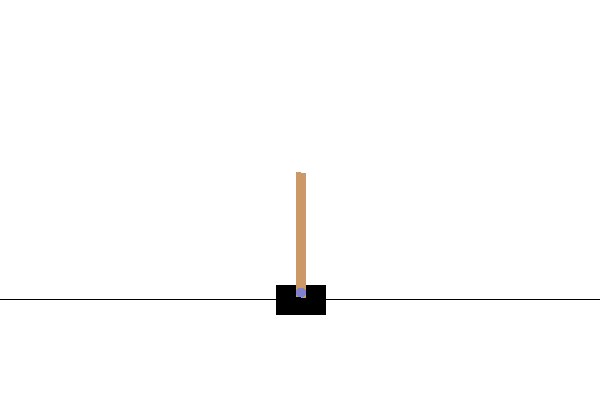
\includegraphics[width=0.8\textwidth]{cartpoleopenai.png}}
  \caption{Representação gráfica do ambiente do \textit{cartpole} em OpenAI}
  \label{fig:cartpole_openai}
\end{center}
\end{figure}

\subsection{\textit{Cartpole} no \textit{Barbell}}
\bruno{pro leitor conseguir saber se é mais facil no barbell, teria que ter visto como foi feito manualmente no ambiente que tem no Gym. Ver comentario acima, sobre discutir melhor exatamente como ele foi implementado (possivelmente mostrando o codigo, mesmo, que nem tu fez com o barbell, abaixo, pra pessoa poder comparar)}

No ambiente do \textit{Barbell}, por este apresentar maior grau de liberdade ao programador, há a necessidade de se
definir todas as partes do agente, todas as partes do ambiente e como elas se relacionam, antes de se dar início ao
treinamento. Através de um \textit{script} no formato YAML que é fornecido à ferramenta, o \textit{framework} cria
as partes do agente, inicializa o ambiente (também com suas partes específicas) e as relações entre as partes do agente e
dos objetos do ambiente (através de juntas) \bruno{a explicacao de como o framework funciona, de forma geral, tem que ir no capto anterior, aonde tu descreve o framework propriamente dito. O capto atual é sobre demonstracoes de como aplicar o framework pra recriar alguns ambientes de exemplo, e comparar o quao facil/dificil/flexivel é a implementacao via teu framework, vs frameworks alternativos que tu descreveu no capto de estado da arte. É tu tentando vender o peixe de que o teu framework é mais facil/tem vantagens, em relacao ao que ja existe}. Todas as definições necessárias para o problema estão presentes no código a seguir:

\begin{minted}[linenos]{yaml}
\bruno{no capto onde tu vai descrever o teu framework, descreve todas essas coisas que fazem parte da sintaxe: uma secao de PARTS, outra de JOINTS, etc, e fala sobre o que vai dentro de cada uma, os possiveis valores pra cada tipo de field (campo box, dentor do PARTS, campo type, dentro de joints, axis, como se especifica as actions, etc etc)}

  AGENT:
    draw_joints: false
    joint_color: [255,0,0,0]
    parts_color: [175,175,175,0]

    PARTS:
      - cart:
          type: box
          initial_position: [12, 9]
          box_size: [2, 1]
          color: [255,63,63,0]
      - pole:
          type: box
          initial_position: [12, 16]
          box_size: [0.1, 2.5]

    JOINTS:
      - connects: [pole, cart]
        type: revolute
        anchor_a: [0, -2.2]
      - connects: [floor, cart]
        type: prismatic
        anchor: [12, 5]
        axis: [1, 0]
        lower_translation: -3
        upper_translation: 3

    ACTIONS:
      - push_cart:
          type: local
          target: cart
          anchor: [0,0]
      - start_pole:
          type: local
          target: pole
          anchor: [0, 2.5]

  ENVIRONMENT:
    gravity: [0, -10]
    floor: none
    OBJECTS:
      - floor:
          type: box
          initial_position: [12, 1]
          box_size: [12, 0.5]
\end{minted}

No código, há a definição das partes do agente (linhas 6-15), dos objetos presentes no cenário (linhas 41-45) e das
juntas que as conectam. Uma junta é necessária para conectar o \textit{cart} ao \textit{pole} (linhas 18-20) e outra
junta, do tipo prismática, cria um eixo paralelo ao chão que torna possível que o \textit{cart} deslize sobre ele
(linhas 21-26). O códido do programa em \textit{python} que se responsabiliza de rodar os testes tem a responsabilidade,
portanto, de fornecer a descrição YAML acima e iniciar cada um dos episódios, fornecendo funções que calculem
a recompensa ao final de cada episódio, que determinem se um episódio chegou ao fim e que escolham qual ação o agente irá
tomar, adicionando, ao início de cada episódio, uma força aleatória ao \textit{pole} que determinará o
comportamento do agente naquele episódio. O código que executa essas ações está explicitado abaixo.


\begin{minted}[linenos]{python}
ai = CartpoleIntelligence()
cartpole = barbell.from_file(os.path.join(
                  os.path.dirname(__file__),
                  'cartpole.yaml')
                  )
cartpole.set_action_function(ai.action_function)
cartpole.set_reset_function(ai.reset_function)
cartpole.set_reward_function(ai.reward_function)
while cartpole.running:
    current_state = cartpole.step()
    if current_state["current_iteration"] == 0:
        cartpole.agent.start_pole((random.randint(-10, 10), 0))
\end{minted}

\section{Lunar Landing}
Exemplo do lunar landing, também recheado de figuras pra encher bastante linguiça.
\section{Robô que atira bolinha (arrumar nome melhor)}
Aqui vai um outro exemplo que eu queria desenvolver que é parecido com aquele vídeo do robô que tu me mostrou uma vez.
O robô pegava uma bola e tinha que acertar uma garrafa de plástico posicionada aleatoriamente na frente dele.
Também recheado de figuras que é pra encher bastante linguiça.



\chapter{Conclusão}
"O meu é melhor do que qualquer outro" em linguagem acadêmica.

% referências
% aqui será usado o environment padrao `thebibliography'; porém, sugere-se
% seriamente o uso de BibTeX e do estilo abnt.bst (veja na página do
% UTUG)
%
% observe também o estilo meio estranho de alguns labels; isso é
% devido ao uso do pacote `natbib', que permite fazer citações de
% autores, ano, e diversas combinações desses

\bibliographystyle{abntex2-alf}
\bibliography{biblio.bib}

\end{document}
